\documentclass[12pt, twoside, openright]{report} %fuente a 12pt, formato doble pagina y chapter a la derecha
\raggedbottom % No ajustar el contenido con un salto de pagina

% MÁRGENES: 2,5 cm sup. e inf.; 3 cm izdo. y dcho.
\usepackage[
a4paper,
vmargin=2.5cm,
hmargin=3cm
]{geometry}

% INTERLINEADO: Estrecho (6 ptos./interlineado 1,15) o Moderado (6 ptos./interlineado 1,5)
\renewcommand{\baselinestretch}{1.15}
\parskip=6pt

% DEFINICIÓN DE COLORES para portada y listados de código
\usepackage[table]{xcolor}
\definecolor{azulUC3M}{RGB}{0,0,102}
\definecolor{gray97}{gray}{.97}
\definecolor{gray75}{gray}{.75}
\definecolor{gray45}{gray}{.45}

% Soporte para GENERAR PDF/A
\usepackage[a-1b]{pdfx}

% ENLACES
\usepackage{hyperref}
\hypersetup{colorlinks=true,
	linkcolor=black, % enlaces a partes del documento (p.e. índice) en color negro
	urlcolor=blue} % enlaces a recursos fuera del documento en azul

% Añadir pdfs como partes del documento
\usepackage{pdfpages}

% Quitar la indentación de principio de los parrafos
\setlength{\parindent}{0em}

% EXPRESIONES MATEMATICAS
\usepackage{amsmath,amssymb,amsfonts,amsthm}

\usepackage{txfonts} 
\usepackage[T1]{fontenc}
\usepackage[utf8]{inputenc}

% Insertar graficas y fotos
\usepackage{tikz}
\usepackage{pgfplots}

\usepackage[spanish, es-tabla]{babel} 
\usepackage[babel, spanish=spanish]{csquotes}
\AtBeginEnvironment{quote}{\small}

% diseño de PIE DE PÁGINA
\usepackage{fancyhdr}
\pagestyle{fancy}
\fancyhf{}
\renewcommand{\headrulewidth}{0pt}
\fancyfoot[LE,RO]{\thepage}
\fancypagestyle{plain}{\pagestyle{fancy}}

% DISEÑO DE LOS TÍTULOS de las partes del trabajo (capítulos y epígrafes o subcapítulos)
\usepackage{titlesec}
\usepackage{titletoc}
\titleformat{\chapter}[block]
{\large\bfseries\filcenter}
{\thechapter.}
{5pt}
{\MakeUppercase}
{}
\titlespacing{\chapter}{0pt}{0pt}{*3}
\titlecontents{chapter}
[0pt]                                               
{}
{\contentsmargin{0pt}\thecontentslabel.\enspace\uppercase}
{\contentsmargin{0pt}\uppercase}                        
{\titlerule*[.7pc]{.}\contentspage}                 

\titleformat{\section}
{\bfseries}
{\thesection.}
{5pt}
{}
\titlecontents{section}
[5pt]                                               
{}
{\contentsmargin{0pt}\thecontentslabel.\enspace}
{\contentsmargin{0pt}}
{\titlerule*[.7pc]{.}\contentspage}

\titleformat{\subsection}
{\normalsize\bfseries}
{\thesubsection.}
{5pt}
{}
\titlecontents{subsection}
[10pt]                                               
{}
{\contentsmargin{0pt}                          
	\thecontentslabel.\enspace}
{\contentsmargin{0pt}}                        
{\titlerule*[.7pc]{.}\contentspage}  


% DISEÑO DE TABLAS.
\usepackage{multirow} % permite combinar celdas 
\usepackage{caption} % para personalizar el título de tablas y figuras
\usepackage{floatrow} % utilizamos este paquete y sus macros \ttabbox y \ffigbox para alinear los nombres de tablas y figuras de acuerdo con el estilo definido. Para su uso ver archivo de ejemplo 
\usepackage{array} % con este paquete podemos definir en la siguiente línea un nuevo tipo de columna para tablas: ancho personalizado y contenido centrado
\newcolumntype{P}[1]{>{\centering\arraybackslash}p{#1}}
\DeclareCaptionFormat{upper}{#1#2\uppercase{#3}\par}

% Diseño de tabla para ingeniería
\captionsetup[table]{
	format=hang,
	name=Tabla,
	justification=centering,
	labelsep=colon,
	width=.75\linewidth,
	labelfont=small,
	font=small,
}

% DISEÑO DE FIGURAS.
\usepackage{graphicx}
\graphicspath{{img/}} %ruta a la carpeta de imágenes

% Diseño de figuras para ingeniería
\captionsetup[figure]{
	format=hang,
	name=Fig.,
	singlelinecheck=off,
	labelsep=colon,
	labelfont=small,
	font=small		
}

% NOTAS A PIE DE PÁGINA
\usepackage{chngcntr} %para numeración continua de las notas al pie
\counterwithout{footnote}{chapter}

% LISTADOS DE CÓDIGO
% soporte y estilo para listados de código. Más información en https://es.wikibooks.org/wiki/Manual_de_LaTeX/Listados_de_código/Listados_con_listings
\usepackage{listings}

% definimos un estilo de listings
\lstdefinestyle{estilo}{ frame=Ltb,
	framerule=0pt,
	aboveskip=0.5cm,
	framextopmargin=3pt,
	framexbottommargin=3pt,
	framexleftmargin=0.4cm,
	framesep=0pt,
	rulesep=.4pt,
	backgroundcolor=\color{gray97},
	rulesepcolor=\color{black},
	%
	basicstyle=\ttfamily\footnotesize,
	keywordstyle=\bfseries,
	stringstyle=\ttfamily,
	showstringspaces = false,
	commentstyle=\color{gray45},     
	%
	numbers=left,
	numbersep=15pt,
	numberstyle=\tiny,
	numberfirstline = false,
	breaklines=true,
	xleftmargin=\parindent
}

\captionsetup[lstlisting]{font=small, labelsep=period}
% fijamos el estilo a utilizar 
\lstset{style=estilo}
\renewcommand{\lstlistingname}{\uppercase{Código}}

\pgfplotsset{compat=1.17} 
%-------------
%	DOCUMENTO
%-------------

\begin{document}
\pagenumbering{roman} % Se utilizan cifras romanas en la numeración de las páginas previas al cuerpo del trabajo
	
%----------
%	PORTADA
%----------	
\begin{titlepage}
	\begin{sffamily}
	\color{azulUC3M}
	\begin{center}
		\begin{figure}[H] %incluimos el logotipo de la Universidad
			\makebox[\textwidth][c]{
\includegraphics[width=16cm]{Portada_Logo.png}}
		\end{figure}
		\vspace{2.5cm}
		\begin{Large}
			Grado en Ingeniería Informática\\			
			2020-2021\\
			\vspace{2cm}		
			\textsl{Apuntes}\\
			\bigskip
		\end{Large}
		 	{\Huge Arquitectura de computadores}\\
		 	\vspace*{0.5cm}
	 		\rule{10.5cm}{0.1mm}\\
			\vspace*{0.9cm}
			{\LARGE Jorge Rodríguez Fraile\footnote{\href{mailto:100405951@alumnos.uc3m.es}{Universidad: 100405951@alumnos.uc3m.es}  |  \href{mailto:jrf1616@gmail.com}{Personal: jrf1616@gmail.com}}}\\ 
			\vspace*{1cm}
	\end{center}
	\vfill
	\color{black}
		
\includegraphics[width=4.2cm]{img/creativecommons.png}\\
		Esta obra se encuentra sujeta a la licencia Creative Commons\\ \textbf{Reconocimiento - No Comercial - Sin Obra Derivada}
	\end{sffamily}
\end{titlepage}

%----------
%	ÍNDICES
%----------	

%--
% Índice general
%-
\tableofcontents
\thispagestyle{fancy}

%--
% Índice de figuras. Si no se incluyen, comenta las líneas siguientes
%-
\listoffigures
\thispagestyle{fancy}

%----------
%	TRABAJO
%----------

\pagenumbering{arabic} % numeración con múmeros arábigos para el resto de la publicación	


%----------
%	COMENZAR A ESCRIBIR AQUI
%----------	

\chapter{Información}
\section{Profesores}
\begin{quote}
  Teorías: José Daniel García jdgarcia@inf.uc3m.es
  josedaniel.garcia@uc3m.es 
  
  Prácticas: ELÍAS DEL POZO PUÑAL, JOSE MANUEL
  PÉREZ LOBATO y DAVID EXPÓSITO SINGH
\end{quote}

\section{Recurso}
\href{https://ubuntu.com/tutorials/install-ubuntu-desktop\#1-overview}{Install
Ubuntu desktop \textbar{} Ubuntu}

\href{https://www.jetbrains.com/es-es/community/education/\#students}{Licencias
educativas gratuitas. Asistencia a la comunidad}

\href{https://en.cppreference.com/w/cpp}{C++ reference}

\href{https://isocpp.org/}{Standard C++}

\href{https://isocpp.org/faq}{Super-FAQ: Standard C++}

\href{http://isocpp.github.io/CppCoreGuidelines/CppCoreGuidelines}{C++
Core Guidelines}

\href{https://www.youtube.com/playlist?list=PLLX-Q6B8xqZ8n8bwjGdzBJ25X2utwnoEG}{Introduction
to OpenMP - Tim Mattson (Intel)}


\part{Teoría}

  \chapter{Módulo 1: Introducción al Diseño de Computadores}

  \section{¿Qué es la arquitectura de computadores?}

  \begin{itemize}
  
  \item
    Son los atributos de un sistema que puede ver el programador, y
    aquellos que no puede ver es la organización del sistema.
  \item
    Es la ciencia y el arte de seleccionar e interconectar componentes
    hardware para que satisfagan los requisitos funcionales, de
    rendimiento y coste.
  \item
    No es lo mismo que el ISA - Instruction Set Arquitecture, al
    principio se creía que era lo mismo, pero la arquitectura de
    computadores es mucho más que diseñar las instrucciones, es
    organización funcional, diseño lógico e implementación. A su vez
    esas tareas son muy complejas. El ISA sirve como límite entre el
    software y el hardware.
  \item
    Estudiarla nos permite comprender las tendencias de la próxima
    década y las limitaciones de los computadores.
  \end{itemize}

  \section{La ley de Moore:}

  Más que una ley es una observación empírica
  \begin{figure}[H]
    \ffigbox[\FBwidth]
    {\caption{Diagrama Ley de Moore}}
    {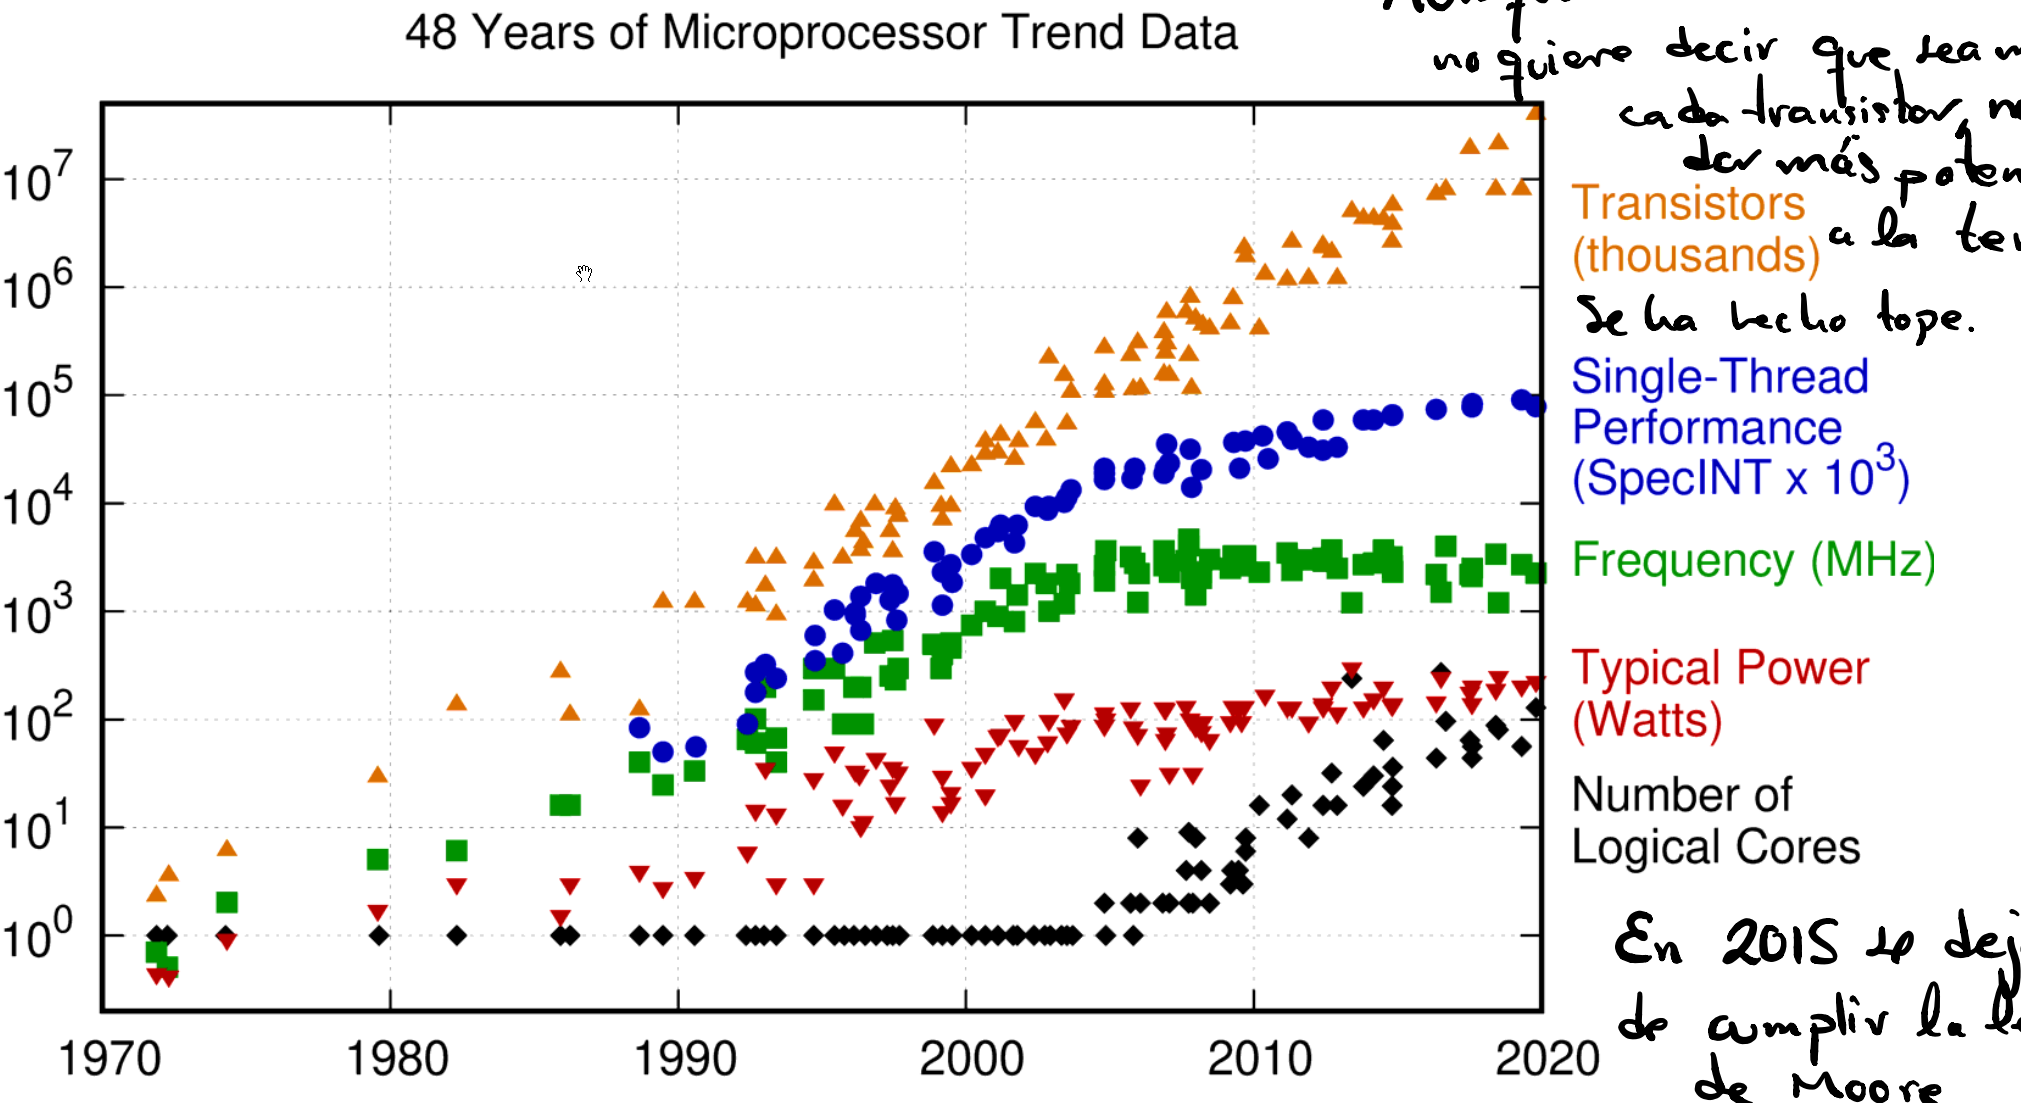
\includegraphics[scale=.2]{Untitled.png}}
  \end{figure}
  \begin{itemize}
  \item
    El número de transistores por chip se duplica cada N meses, donde N
    varía entre 12 y 24. Aumenta exponencialmente.
  \item
    En 2015 se dejó de cumplir. No somos capaces de aumentar la
    frecuencia.
  \item
    Aunque han aumentado los transistores no quiere decir que sea más
    rápido cada uno de ellos, ya que se llega un punto en el que no
    puede dar más potencia debido al problema de la temperatura.
  \item
    Evolución del rendimiento:
    \begin{figure}[H]
      \ffigbox[\FBwidth]
      {\caption{Evolución del del rendimiento}}
      {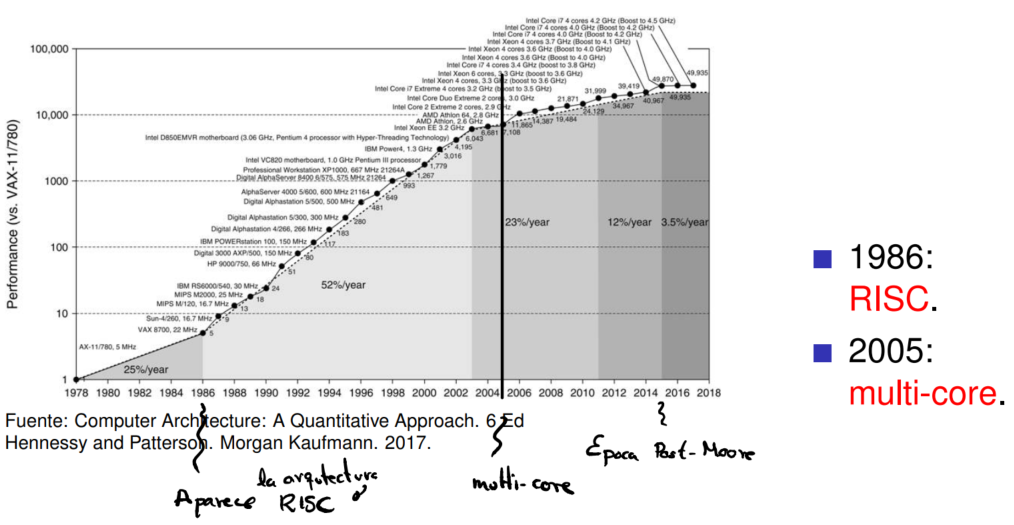
\includegraphics[scale=.35]{Untitled 1.png}}
    \end{figure}
  \end{itemize}

  \section{RISC:}

  Aparece en 1986 como una nueva arquitectura.

  \begin{itemize}
  
  \item
    Permitió una mejora de la capacidad disponible. Hasta el punto que
    un microprocesador de alta gama era más potente que una
    supercomputadora de 10 años atrás.
  \item
    Se mejoró el ratio coste/rendimiento, lo que dio lugar a nuevos
    computadores. En los 80 PC y Workstation, y en los 00
    smartphones, tablets y grandes centros de datos.
  \item
    Fue una revolución, permitió dominar los computadores basados en
    microprocesadores, gracias a la mejora continua de semiconductores.
  \item
    El rendimiento crecía 52\% al año hasta el 2003.
  \end{itemize}
\pagebreak
  \section{Perspectiva histórica:}

  \subsection{Primera revolución (70's): El microprocesador}

    \begin{itemize}
    \item
      Primer microprocesador.
      \begin{figure}[H]
        \ffigbox[\FBwidth]
        {\caption{Primer microprocesador}}
        {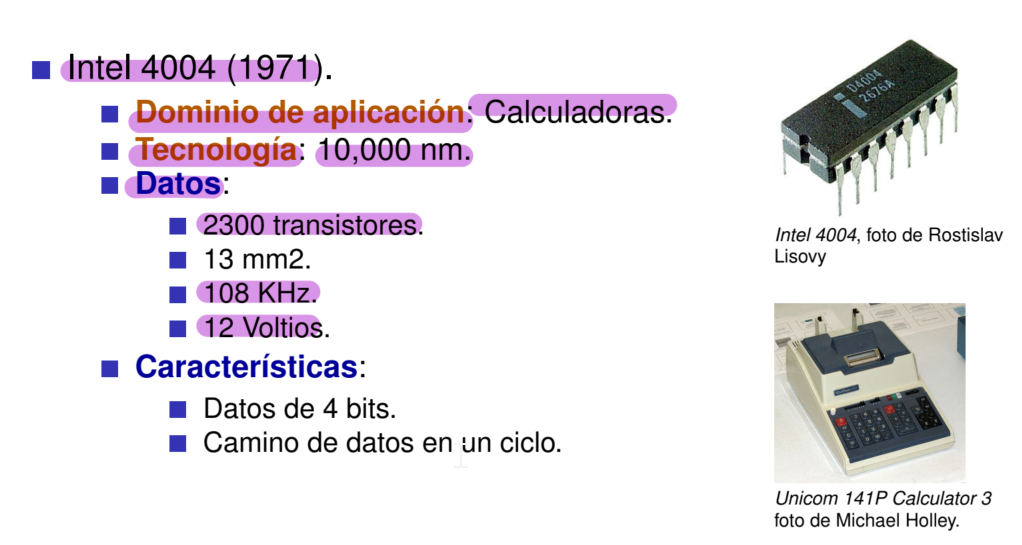
\includegraphics[scale=.25]{Untitled 2.png}}
      \end{figure}
    \item
      Fue posible al poder poner suficientes transistores, 25000, en un
      único chip para un procesador de 16 bits.
    \item
      Era más barato, todo en un chip, y más rápido, no hacía falta
      tantas salidas del chip al estar todo junto.
    \item
      Aparecen computadores de escritorio, portátiles, consolas,
      descodificadores, etc.
    \item
      Se mejoraron las supercomputadoras como agregación de muchas
      placas con procesadores estándar.
    \end{itemize}
  
    \subsection{Segunda revolución (80's): Paralelismo a nivel de instrucción}

    \begin{itemize}
    \item
      ILP -- Instruction Level Parallelism.
    \item
      El hardware tiene recursos que se pueden usarse en paralelo.
      Mientras se realiza una parte para una, se hace otra para otro.
    \item
      Elementos:

      \begin{itemize}
      
      \item
        Segmentación o Pipeline: Dividir el diseño del procesador en
        distintas partes físicas que se pueden usar por separado. Se
        incrementa la frecuencia de reloj.
      \item
        Caches: Necesaria para incrementar las frecuencias, para esperar
        menos a los datos de disco.
      \item
        Coma flotante: Integradas en el chip, junto a la unidad
        aritmética general.
      \item
        Incremento en la profundidad del pipeline, más etapas, y
        especulación de salto, intenta adivinar que rama se van a tomar.
      \item
        Emisión múltiple: Arquitecturas superescalares, captar más de
        una instrucción por ciclo de reloj, entre 2 y 4 instrucciones.
      \item
        Planificación dinámica: Ejecución fuera del orden programado,
        con el objetivo de que sea más rápido y funcione igual.
      \end{itemize}
    \item
      Culminación de procesadores de un núcleo.
      \begin{figure}[H]
        \ffigbox[\FBwidth]
        {\caption{Culminación de procesadores de un núcleo}}
        {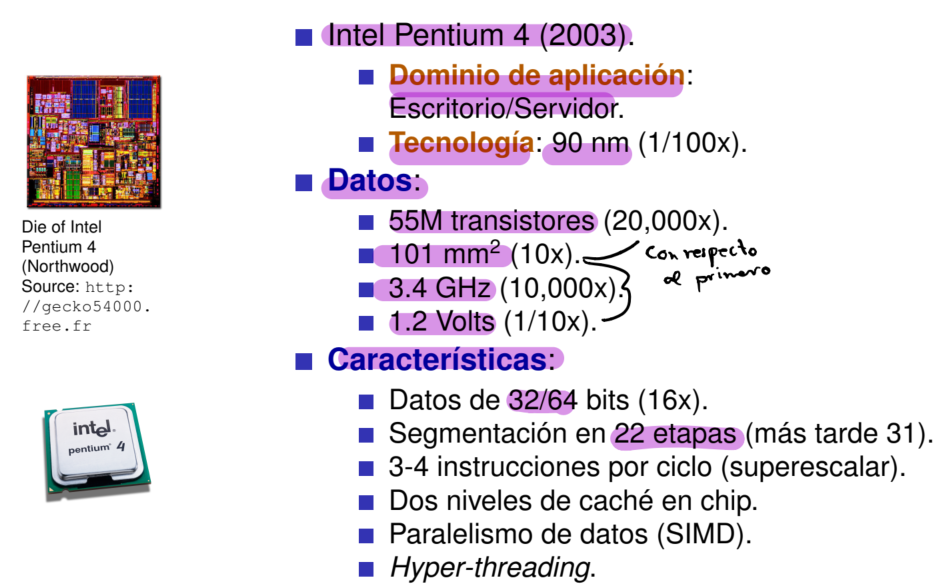
\includegraphics[scale=.25]{Untitled 3.png}}
      \end{figure}
    \end{itemize}
    
    \subsection{Tercera revolución: Paralelismo de datos y de hilos}

    \begin{itemize}
    \item
      Soporte a paralelismo explícito de datos y de hilos.
    \item
      El hardware ofrece recursos paralelos y el software especifica su
      uso.
    \item
      El paralelismo deja de ser ocultado por el hardware.
    \item
      La razón es que los beneficios del ILP son cada vez menores, no
      pueden hacer un núcleo de ejecución más complicado, pero pueden
      meter más transistores.
    \item
      Se introducen más cores y se mejora la memoria caché del chip.
    \item
      Elementos:

      \begin{itemize}
      
      \item
        Instrucciones vectoriales, que dan muy buen resultado en
        aplicaciones multimedia.
      \item
        Soporte general para aplicaciones.
      \end{itemize}
    \pagebreak
    \item Procesadores multi-core.
      \begin{figure}[H]
        \ffigbox[\FBwidth]
        {\caption{Procesadores multi-core}}
        {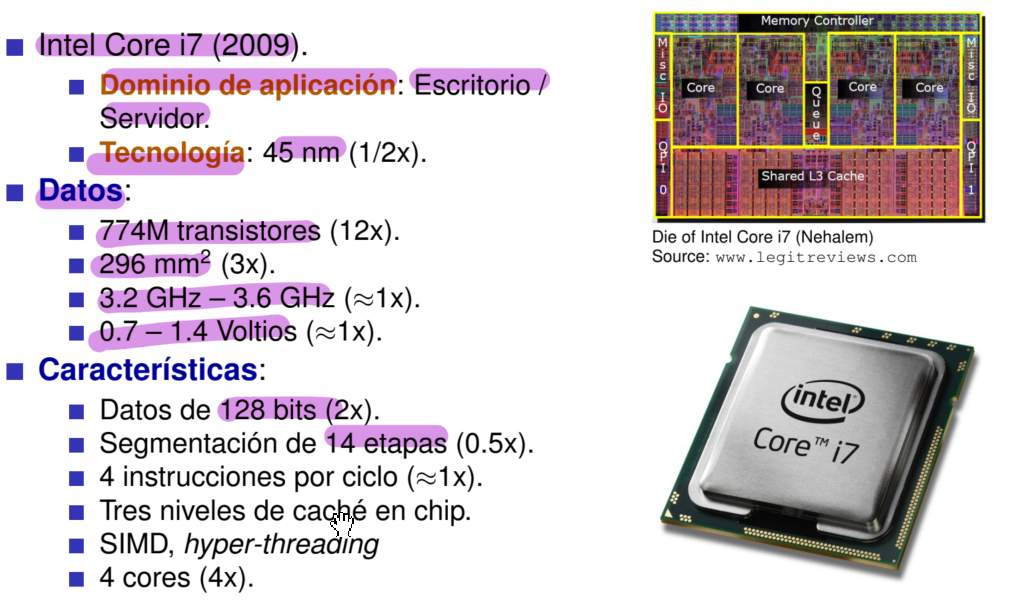
\includegraphics[scale=.25]{Untitled 4.png}}
      \end{figure}
    \end{itemize}

  \section{Tendencias arquitectónicas}

  \begin{itemize}
  
  \item ILP - Paralelismo a nivel de instrucción: Permite ejecutar varias
    instrucciones, pero 2003-2005 no se puede mejorar
    significativamente.

    \begin{itemize}
    
    \item
      El hardware y el compilador oculta detalles al programador, por lo
      que este tiene una vista secuencial muy simplificada del hardware.
    \end{itemize}
  \item
    Con la aparición de los multi-core surgen nuevos tipos de
    procesamiento, pero estos requieren reestructurar las aplicaciones
    para incrementar el rendimiento:

    \begin{itemize}
    
    \item
      Paralelismo a nivel de dato -- DLP
    \item
      Paralelismo a nivel de hilo -- TLP
    \item
      Paralelismo a nivel de petición -- RLP
    \end{itemize}
  \end{itemize}

  \section{Paralelismo}

  \begin{itemize}
  
  \item
    Forma de~computación~en la cual varios cálculos pueden realizarse
    simultáneamente, basado en el principio de dividir los problemas
    grandes para obtener varios problemas pequeños, que son
    posteriormente solucionados en paralelo.

    \begin{itemize}
    
    \item
      La velocidad de las máquinas secuenciales, no nos permiten
      alcanzar velocidades de procesado demasiado altas por limitaciones
      físico.

      \begin{itemize}
      
      \item
        Por ejemplo, una máquina secuencial de 1 TFLOP, no es factible
        con una aproximación secuencial.
      \end{itemize}
    \end{itemize}
    \pagebreak
  \item
    Aparece como principal mecanismo de diseño de computadores, contra
    las restricciones de coste y consumo de energía.
  \item
    Tipos de paralelismo en las aplicaciones:

    \begin{itemize}
    
    \item
      Paralelismo de datos: Se aplica la misma operación a distintos
      datos.
    \item
      Paralelismo de tareas: Se ejecutan distintas operaciones.
    \end{itemize}
  \item
    Tipos de paralelismo hardware:

    \begin{itemize}
    
    \item
      ILP - Paralelismo a Nivel de Instrucción: Explota el paralelismo
      de datos con ayuda del compilador.
    \item
      Arquitecturas vectoriales y GPU: Explotan el paralelismo de datos
      aplicando la misma operación a varios datos en paralelo.
    \item
      TLP - Paralelismo a Nivel de Hilo: Explota el paralelismo de datos
      o tareas en hardware altamente acoplado. Permite interacciones
      entre hilos.

      \begin{itemize}
      
      \item
        Por ejemplo, un procesador con varios cores.
      \end{itemize}
    \item
      RLP - Paralelismo a Nivel de Petición: Explota el paralelismo
      entre tareas altamente desacopladas.

      \begin{itemize}
      
      \item
        Cuando hay varios computadores en una red y cada uno de ellos
        procesa una petición distinta de un servidor.
      \end{itemize}
    \end{itemize}
  \end{itemize}

  \section{Clasificación de computadores}

  
    \subsubsection{Dispositivos móviles personales}

    \begin{itemize}
    
    \item
      Dispositivos sin cables con una interfaz de usuario multimedia.

      \begin{itemize}
      
      \item
        Dispositivos móviles, tablets, etc.
      \end{itemize}
    \item
      Precio: \$100 -- \$1000.
    \item
      Precio de procesador: \$10 -- \$100.
    \item
      Factores críticos:

      \begin{itemize}
      
      \item
        Coste, a un centenar de dólares.
      \item
        Energía, ya que debe durar suficiente la batería.
      \item
        Rendimiento, realizar las tareas en un tiempo adecuado.
      \item
        Tiempo de respuesta, interfaces de usuario rápidas.
      \end{itemize}
    \end{itemize}
    \subsubsection{Computadores de escritorios}

    \begin{itemize}
    
    \item
      Diseñados para ofrecer un buen rendimiento a los usuarios.

      \begin{itemize}
      
      \item
        Desde ultra-books hasta estaciones de trabajo.
      \item
        Más de 50\% son portátiles.
      \end{itemize}
    \item
      Precio: \$300 -- \$2500.
    \item
      Precio de procesador: \$50 -- \$500.
    \item
      Factores críticos:

      \begin{itemize}
      
      \item
        Precio-Rendimiento, están dispuestos a pagar más si van a
        obtener mejor rendimiento.
      \item
        Energía.
      \item
        Rendimiento de gráficos.
      \end{itemize}
    \end{itemize}
    \subsubsection{Servidores}

    \begin{itemize}
    
    \item
      Usados para ejecutar aplicaciones de gran escala y dar servicio a
      múltiples usuarios de forma simultánea.

      \begin{itemize}
      
      \item
        Han crecido mucho desde los 80 y sustituyeron a los mainframes.
      \end{itemize}
    \item
      Precio: \$5,000 -- \$10,000,000.
    \item
      Precio de procesador: \$200 -- \$2,000. Hay muchos procesadores.
    \item
      Factores críticos:

      \begin{itemize}
      
      \item
        Throughput (tasa de procesamiento), las peticiones procesadas
        por unidad de tiempo.
      \item
        Disponibilidad, que sean accesibles en cualquier momento.
      \item
        Escalabilidad, que permite hacerlo más grande mejorando las
        prestaciones.
      \item
        Energía, ya que suponen un gran gasto en electricidad.
      \end{itemize}
    \end{itemize}
    \pagebreak
    \subsubsection{Clusters / Computadores a Escala de Almacén - Warehouse Scale Computers (WSC)}

    \begin{itemize}
    
    \item
      Pasillos y pasillos de armarios llenos de placas con memoria,
      disco y procesador conectadas en LAN. Cada uno ejecuta su sistema
      operativo.
    \item
      Una colección de computadores conectados mediante Red de Área
      Local - LAN que actúa como un computador más grande.

      \begin{itemize}
      
      \item
        Alcanza más popularidad debido a crecimiento de SaaS (Software
        as a Service).
      \item
        Cada nodo ejecuta su propio sistema operativo.
      \item
        A partir de 1000 nodos se considera WSC.
      \end{itemize}
    \item
      Precio: \$100,000 -- \$200,000,000.
    \item
      Precio de procesador: \$50 -- \$250.
    \item
      Factores críticos:

      \begin{itemize}
      
      \item
        Precio-Rendimiento.
      \item
        Throughput (tasa de procesamiento).
      \item
        Proporcionalidad en energía.
      \end{itemize}
    \end{itemize}
    
    \subsubsection{Empotrados}

    \begin{itemize}
    
    \item
      Computador dentro de otro sistema que ejecuta aplicaciones
      preestablecidas. Un solo sistema puede tener cientos de pequeños
      microprocesadores, por eso deben ser baratos.

      \begin{itemize}
      
      \item
        Lavaplatos, consola de videojuegos, MP3, ...
      \end{itemize}
    \item
      Precio: \$10 -- \$100,000.
    \item
      Precio de procesador: \$0.01 -- \$100.
    \item
      Factores críticos:

      \begin{itemize}
      
      \item
        Precio, ya que no es lo fundamental.
      \item
        Energía.
      \item
        Rendimiento de aplicación específica, ya que hace una función
        específica.
      \end{itemize}
    \end{itemize}
  \pagebreak
  \subsection{Mainframe}

  Tipo de computador hasta los 70 de gran escala que usaban las
  compañías para el back office. Estaban muy optimizados para
  procesamiento batch, por lotes.

  \subsection{Taxonomía de Flynn}

  Clasificación de arquitecturas paralelas posibles:

  \begin{itemize}
  
  \item
    SISD - Single Instruction Single Data Stream: Una sola instrucción
    sobre un único dato.

    \begin{itemize}
    
    \item
      Monoprocesador
    \end{itemize}
  \item
    SIMD -- Single Instruction Multiple Data Stream: Una única
    instrucción sobre varios datos.

    \begin{itemize}
    
    \item
      Alternativas: Procesadores vectoriales, extensiones multimedia y
      GPU.
    \end{itemize}
  \item
    MISD -- Multiple Instruction Single Data: No se conocen
    implementaciones comerciales. Nunca se ha construido.
  \item
    MIMD -- Multiple Instruction Multiple Data: Múltiples instrucciones
    sobre múltiples datos. Cada procesador opera sobre sus propios
    datos, permite el Paralelismo de tareas.

    \begin{itemize}
    
    \item
      También se puede incluir el Paralelismo a Nivel de Hilo como en
      las arquitecturas multi-core o el Paralelismo a Nivel de Petición
      de los clústeres y WSC.
    \item
      Es más caro que el SIMD, pero es más flexible y general.
    \item
      Requiere que las tareas a ejecutar sean suficientemente
      complicadas.
    \end{itemize}
  \end{itemize}

  \chapter{Módulo 2: Evaluación del rendimiento de sistemas informáticos}
  \section{Tendencias tecnológicas}

  \begin{itemize}
  
  \item
    Impacto de la tecnología: Los cambios tecnológicos tienen impacto en
    los mecanismos de implementación de la ISA -- Arquitectura del Juego
    de Instrucciones.

    \begin{itemize}
    
    \item
      Tecnología de circuitos integrados:

      \begin{itemize}
      
      \item
        Densidad de transistores: 35\% anual.
      \item
        Tamaño del dado: 10\%-20\% anual.
      \item
        Efecto combinado: 40\%-55\% anual, pero se dejó de cumplir (Ley
        de Moore).
      \end{itemize}
    \item
      Capacidad DRAM:

      \begin{itemize}
      
      \item
        25\%-40\% anual (reduciéndose).
      \end{itemize}
    \item
      Capacidad Flash:

      \begin{itemize}
      
      \item
        50\%-60\% anual
      \item
        8-10 veces más barato por bit que DRAM
      \end{itemize}
    \item
      Capacidad de discos magnéticos:

      \begin{itemize}
      
      \item
        5\% anual (últimos años).
      \item
        8-10 veces más barato por bit que Flash.
      \item
        200-300 veces más barato que DRAM.
      \end{itemize}
    \end{itemize}
  \item
    Ancho de banda -- Throughput: Cantidad de trabajo realizada por
    unidad de tiempo.

    \begin{itemize}
    
    \item
      Procesadores: Instrucciones por segundo. Incremento entre 32.000 y
      40.000 veces.
    \item
      Memoria y discos: bytes o bits transferidos por unidad de tiempo.
      Incremento entre 300 y 1.200 veces.
    \end{itemize}
  \item
    Latencia: Tiempo entre inicio y fin de un evento.

    \begin{itemize}
    
    \item
      Procesadores: Desde que se ejecuta hasta que termina. Incremento
      entre 50 y 90 veces.
    \item
      Memorias y discos: Desde que comienza la lectura hasta que
      termina. Incremento entre 6 y 8 veces.
    \end{itemize}
  \item
    El ancho de banda ha aumentado mucho con respecto a la latencia.

   
    \begin{figure}[H]
      \ffigbox[\FBwidth]
      {\caption{Ancho de banda vs. Latencia}}
      {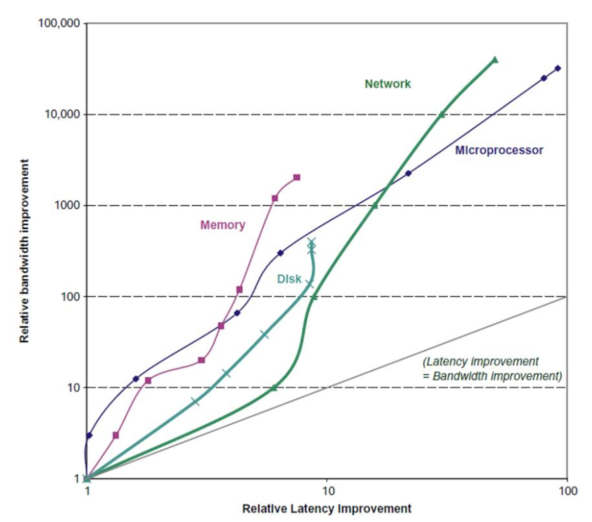
\includegraphics[scale=.4]{Untitled 5.png}}
    \end{figure}
  \end{itemize}

  \section{Tendencias en potencia y energía}

  \begin{itemize}
  
  \item
    El coste se mide en Energía. \(E= P \cdot t\)

    \begin{itemize}
    
    \item
      No siempre el más potente es que más energía consume, pero cuando
      ocurre hay que plantearse si merece la pena.
    \end{itemize}
  \item
    En la tecnología CMOS, el consumo de energía viene de la conmutación
    de transistores.
  \item
    Energía dinámica: Cantidad de energía necesaria para conmutar.

    
    
      \(E_d \approx \frac 1 2 \cdot X_c\cdot V^2\)

      La reducción del voltaje mejora mucho la Energía dinámica, con el
      tiempo se ha pasado de 5 a 1V.

    \item
    Potencia dinámica: Depende de la frecuencia de conmutación.

    
    
      \(P_d \approx \frac 1 2 \cdot X_c\cdot V^2\cdot f\)

    \begin{itemize}
      
      \item
        Xc: Carga capacitiva. Depende del número de transistores.
      \item
        V: Voltaje.
      \item
        f: frecuencia
      \end{itemize}
      \pagebreak
    \item
    La evolución ha estado dominada por el incremento de número de
    transistores e incremento de frecuencia, lo que ha incrementado la
    potencia, pero también la energía.

    \begin{itemize}
    
    \item
      El incremento de la energía hasta los 95 W provoca una gran
      cantidad de calor que debemos disipar y se ha alcanzado el límite
      de enfriamiento por ventilación.
    \end{itemize}
  \item
    Eficiencia energética:

    \begin{itemize}
    
    \item
      Desactivación de reloj de las unidades inactivas.
    \item
      Escalado dinámico de voltaje y frecuencia (DVFS)
    \item
      Modos de bajo consumo en memoria y discos, aunque requieren
      reactivación que puede tardar.
    \item
      Overclocking automático, si es seguro.
    \end{itemize}
  \end{itemize}

  \section{Tendencias en coste}

  \begin{itemize}
  
  \item
    El coste de fabricación de un computador se reduce a lo largo del
    tiempo.

    \begin{itemize}
    
    \item
      Principio de la curva de aprendizaje: Se comienza siendo
      ineficiente y con el tiempo se va mejorando el proceso de
      fabricación. También hay que tener en cuenta el coste de
      ingeniería o diseño.

      \begin{itemize}
      
      \item
        Si se dobla el rendimiento se divide a la mitad el coste.
      \item
        DRAM: Promedio de caída anual del 40\% en coste y precio
      \end{itemize}
    \item
      Volumen: Cuantos más se fabriquen de una vez, el coste por unidad
      se reduce.

      \begin{itemize}
      
      \item
        Decremento del 10\% en coste si se dobla volumen.
      \end{itemize}
    \item
      Venta por múltiples fabricantes de mismo producto: La competencia.
    \end{itemize}
  \item
    Dado: Cada uno de los circuitos -chips impresos sobre la oblea.
  \item
    Oblea: Material semiconductor donde se imprimen los circuitos.
\pagebreak
    \begin{itemize}
    \item
      Coste

      \begin{figure}[H]
        \ffigbox[\FBwidth]
        {\caption{Costes por chip}}
        {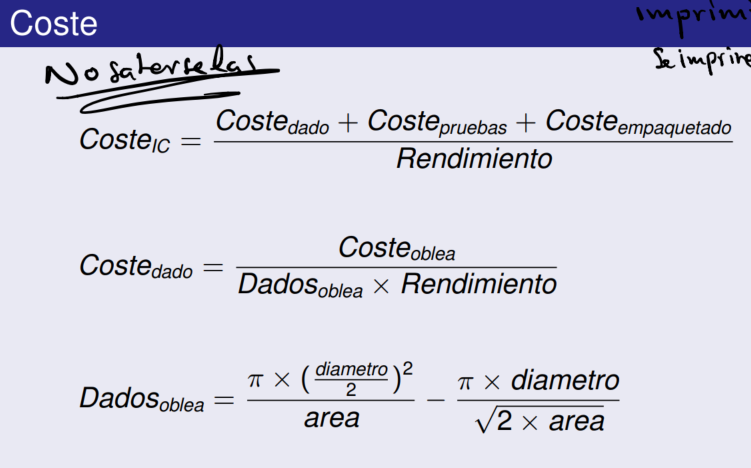
\includegraphics[scale=.35]{Untitled 6.png}}
      \end{figure}
    \end{itemize}
  \end{itemize}


  


 \section{Evaluación del rendimiento}

  \subsection{Métricas de rendimiento}

  \begin{itemize}
  
  \item
    Velocidad de ejecución: Tiempo en el que se ejecuta un programa o
    transacción. Se trata de reducir el tiempo de ejecución, lo que
    aumenta la tasa de procesado.
  \item
    Rendimiento: Es una métrica inversa al tiempo de ejecución.
    \(R= \frac 1 T\) Alto rendimiento -\textgreater{} Bajo tiempo de
    ejecución.
  \item
    Aceleración: Veces que x es más rápido que y.
    \(n=\frac {T(x)} {T(y)}=\frac {R(y)} {R(x)}\) No está claro si están
    bien.
  \item
    La única métrica fiable para comparar rendimiento de computadores es
    la ejecución de programas reales, cualquier otra conduce a errores,
    hay que probar con lo que buscamos rendimiento.
  \item
    Tiempo de ejecución.

    \begin{itemize}
    
    \item
      Tiempo de respuesta: Tiempo total transcurrido.
    \item
      Tiempo de CPU: Tiempo que la CPU ha estado ocupada.
    \end{itemize}
  \end{itemize}

  \subsection{Benchmarks}

  \begin{itemize}
  
  \item
    Aplicación o conjunto de aplicaciones usadas para evaluar
    rendimiento.
  \item
    El rendimiento de un computador depende de la carga de trabajo con
    la que se evalúa. Los computadores están adaptados a cargas
    específicas (servidores web, servidores de bases de datos,
    computador personal, multicomputadores, \ldots).
  \item
    Aproximaciones: Malas al no ser programas reales, el arquitecto y el
    compilador pueden engañar

    \begin{itemize}
    
    \item
      Kernels: Partes pequeñas de aplicaciones reales.
    \item
      Programas de juguete: Programas cortos.
    \item
      Benchmarks sintéticos: Inventados para medir el rendimiento, para
      representar aplicaciones reales.
    \end{itemize}
  \item
    Algunos benchmarks para:

    \begin{itemize}
    
    \item
      Empotrados: Dhrystone y EEMBC.
    \item
      Desktop: SPEC2017(mezcla de programas reales con unos datos
      concretos)
    \item
      Servidores: SPECWeb, SPECSFS o TPC.
    \end{itemize}
  \end{itemize}

  \subsection{Ley de Amdahl}

  \begin{itemize}
  
  \item
    El incremento de rendimiento obtenido usando un modo de ejecución
    más rápido está limitado por la fracción de tiempo que se puede usar
    dicho modo.
  \item
    Cuando mejora el rendimiento depende mucho de cuánto tiempo se
    ejecuta. Hay que optimizar las que más tiempo va a estar
    ejecutándose.
  \item
    Speedup o aceleración: Cuantas veces es mejor la mejora con respecto
    al original. Ratio entre el rendimiento mejorado y el rendimiento
    original.


    $$S=\frac {R_{mejorado}} {R_{original}}=\frac {T_{original}} {T_{mejorado}}$$

    $$S=\frac 1 {(1-F)+\frac F S} \textit{F: fracción mejorable,}
    \frac {T_{a\space mejorar}} {T_{total}}$$

    \begin{itemize}
    \item
      El speedup depende exclusivamente de la fracción de mejora y el
      speedup de la mejora.
      \begin{figure}[H]
        \ffigbox[\FBwidth]
        {\caption{Procesadores vs. Speedup}}
        {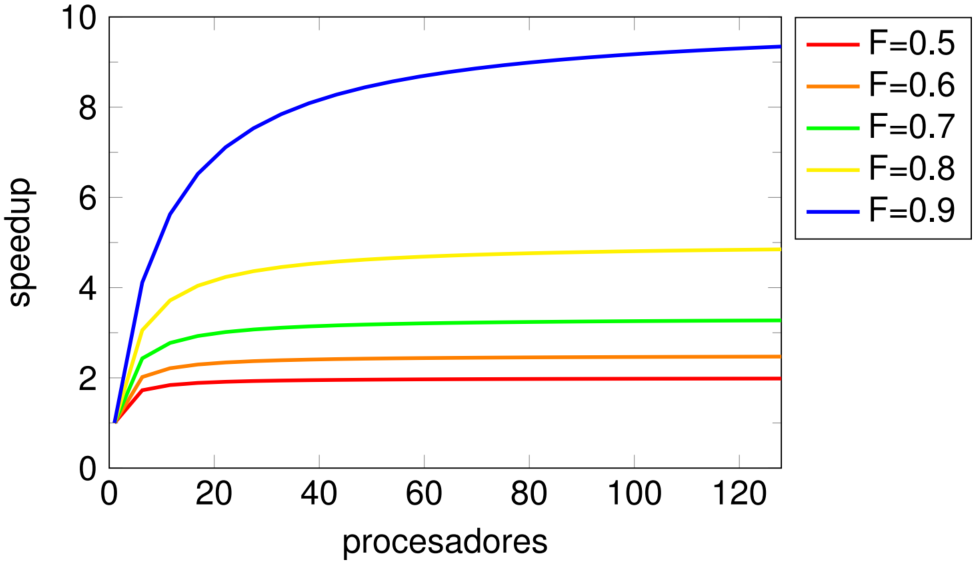
\includegraphics[scale=.26]{Untitled 7.png}}
      \end{figure}
    \end{itemize}
  \item
    Se debe optimizar:

    \begin{itemize}
    
    \item
      Dentro del procesador: la ruta de datos.
    \item
      En el juego de instrucciones: las instrucciones más frecuentes.
    \item
      En el diseño de la jerarquía de memoria, la programación y la
      compilación: hay que explotar la localidad de las referencias. El
      90\% del tiempo se está ejecutando el 10\% del código.
    \end{itemize}
  \end{itemize}

  \subsection{Rendimiento del procesador}

  \begin{itemize}
  
  \item
    Cada instrucción ocurre en varios ciclos de reloj.
  \item
    CPI: Ciclos por instrucción. \(CPI = \frac {ciclosCPU} {IC}\)
  \item
    IC: Instrucciones ejecutadas.
  \item A veces se pone P de Periodo en vez de T. $T=\frac 1f$
  
  $$tiempoCPU = \frac {ciclosCPU} f= CPI\cdot IC\cdot T$$ 
  
  

    \begin{itemize}
    
    \item
      Si se reducen un 10\% cualquiera de los 3 factores se reduce un
      10\% el tiempo de ejecución.
    \end{itemize}
  \item
    La frecuencia relativa de las instrucciones tiene impacto en la
    ejecución del programa.


    

    $$CPI_{global}=\sum_{i=1}^{n} \frac {IC_i} {IC} \times CPI_i$$

    \end{itemize}

  \chapter{Módulo 3 Paralelismo a nivel de instrucción}


  
  \section{Segmentación (Pipeline)}

  Técnica de implementación de los procesadores en la que la ejecución
  de múltiples instrucciones se solapa en el tiempo.

  La instrucción se divide en ciclos, se hacen suboperaciones simples,
  se van ejecutando de forma escalonada.

  \begin{itemize}
  
  \item
    Efectos:

    \begin{itemize}
    
    \item
      Aumenta la tasa de procesamiento (Throughput), al ser de forma
      escalonada, termina una operación por ciclo.
    \item
      No disminuye la latencia, cada instrucción individual tarda lo
      mismo o más, lo que pasa es que terminan más operaciones por
      unidad de tiempo. Una instrucción 5 etapas, 5 ciclos.
    \item
      Un pipeline de profundidad n, multiplica por n el ancho de banda
      necesario de la versión sin pipeline. Se necesita más dado que las
      etapas de captación y memoria acceden a memoria y se van
      solapando.

      \begin{itemize}
      
      \item
        Se solventa y evitan problemas de memoria con una caché de datos
        y una caché de instrucciones.
      \end{itemize}
    \item
      Distintas instrucciones en el pipeline no deben usar el mismo
      recurso en el mismo ciclo.

      \begin{itemize}
      
      \item
        Se introducen registros de pipeline entre etapas, donde se
        almacenan temporalmente los datos de la etapa anterior para
        usarlo en la siguiente. Hay tantos registro por etapa como
        salidas de la etapa.
      \end{itemize}
    \item
      Para evitar conflictos en los registros, todos escriben en la
      primera mitad de ciclo y leen en la segunda mitad de ciclo.
    \end{itemize}
  \item
    Tratamos un modelo simplificado con solo 5 etapas (ejem: Intel 20-28
    etapas)
    \pagebreak
    \item
    Etapas:
    \begin{figure}[H]
      \ffigbox[\FBwidth]
      {\caption{Etapas de la Pipeline}}
      {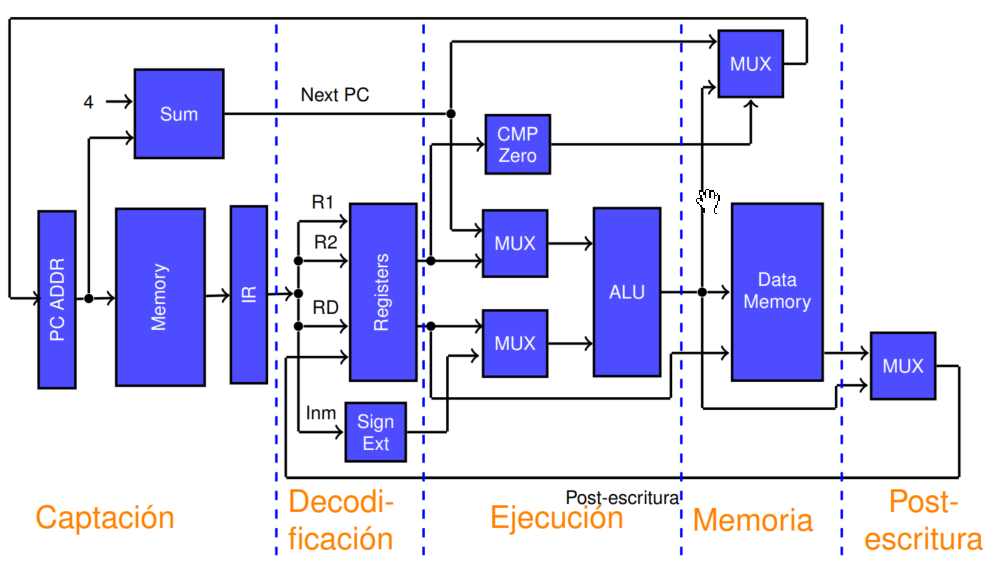
\includegraphics[scale=.3]{Untitled 8.png}}
    \end{figure}
    \begin{itemize}
    
    \item
      Captación (Fetch): Leer la instrucción de la memoria de
      instrucciones y lo carga en el IR.

      \begin{itemize}
      
      \item
        Leer el PC en memoria y se guarda en el IR.
      \item
        Actualización de PC, se suma un valor fijo.
      \end{itemize}
    \item
      Decodificación (Decode): Mira código de operación y obtiene el
      valor de los operandos del banco de registros.

      \begin{itemize}
      
      \item
        Se utiliza el campo de código de operación para activar las
        señales de control.
      \item
        Se leen los registros correspondientes y se preparan para entrar
        en la ALU.
      \item
        También se aplica extensión de signo, 16-32 bits, y el cálculo
        de la dirección de salto.
      \end{itemize}
    \item
      Ejecución (Execution): Se hacen las operaciones en la ALU.

      \begin{itemize}
      
      \item
        Se utiliza la ALU para operar los valores preparados previos.
      \item
        También se usa la ALU para calcular direcciones de memoria.
      \end{itemize}
    \item
      Memoria (Memory): Escritura o lectura de memoria de datos.

      \begin{itemize}
      
      \item
        Se lee o escribe en memoria.

        
          Leer: Se pasa la dirección y sale el dato.
          Escritura: Se pasa la dirección y el dato a escribir.
      \end{itemize}
    \item
      Post-escritura (Write-back): Actualización de banco de registros,
      guarda los resultados.
    \item
      Se escribe la salida de la ALU o de la memoria de datos en el
      banco de registros.
    \end{itemize}
  \end{itemize}


  \section{Riesgos:}

Situación que impide que la siguiente instrucción pueda comenzar en el
ciclo de reloj previsto.

Provocan una reducción del rendimiento.

\subsection{Tipos de riesgos:}
\subsubsection{Riesgo estructural} Cuando el hardware no puede soportar todas las posibles secuencias de instrucciones.
    \begin{itemize}
      \item En un mismo ciclo dos etapas hacen uso del mismo recurso.
      \item Una de esas etapas debería esperar hasta que el recurso este libre.
      \item Razones:
          \begin{itemize}
            \item Unidades funcionales no totalmente segmentadas, cuando hay operaciones que hacen varios ciclos en el mismo recurso. Se podría subdividir en subetapas.
            \item Unidades funcionales no duplicadas. Se podría dividir en instrucciones más cortas, de esa manera, en cada ciclo completa un aparte dentro de ese recurso.
          \end{itemize}
   
      \item Es evitable, pero encarece el hardware.
      \item Se resuelve por hardware, dos caches instrucciones y datos.
    \end{itemize}
    
    \subsubsection{Riesgo de datos} Cuando la segmentación modifica el orden de accesos de lectura/escritura a los operandos.
    \begin{itemize}
      \item Tratamos de leer o escribir un dato que todavía no se ha guardado o leído por estar en etapas intermedias. Se leen en la 2º etapa y se escribe en la 5º etapa.
      \item Clasificación según la relación entre instrucciones:
      \begin{itemize}
        \item RAW: Lectura después de escritura, conocida como Dependencia verdadera. No pueden ejecutarse en paralelo ni solaparse.
        
        Soluciones:
        \begin{itemize}
          \item Que el hardware lo detecte.
          
          \item Que lo controle el compilador, introducción entre medias otras etapas.
        \end{itemize}    
          
       
        \item WAR: Escritura después de lectura, conocida como Anti dependencia, va al revés del orden habitual.
        
        No puede ocurrir en un MIPS con 5 etapas, dado que lectura es el 2º y escritura en la 5º.
        \item WAW: Escritura después de escritura, conocido como dependencia de salida.
        
        No puede ocurrir en un MIPS con pipeline de 5 etapas, ya que la escritura es siempre en la 5 etapa.
      \end{itemize}
          
      \item Soluciones a los riesgos de datos:
      \begin{itemize}
        \item Se puede resolver con detenciones: Se retrasan las instrucciones hasta que se escribe el dato.
        \item Se resuelve con 1ª mitad escritura y 2ª mitad leer. Además de Forwarding.
        \item Dependencias RAW:
        \begin{itemize}
          \item Envío Adelantado (Forwarding): Técnica para evitar algunas detenciones de datos, no hace falta esperar.

          Consiste en tomar los valores tras al etapa de Ejecución y Memoria, en los registros de pipeline.

          No todos los riesgos se pueden evitar, no se puede leer antes de que se haya escrito incluso en los 
          registros de pipeline.

          \item Dependencia WAR y WAW:

          Renombrado de registros. 
        \end{itemize}
                
      \end{itemize}

    \end{itemize}
    
    \subsubsection{Riesgo de control} Se produce en una instrucción de alteración del PC, contador de programa.
    \begin{itemize}
      \item Las bifurcaciones son problemáticas porque no sabemos si se tomara o no hasta que se resuelva la condición, y no se puede preparar las instrucciones.
      \item Terminología:
          
      - Bifurcación tomada: modifica el PC.
         
      - Bifurcación no tomada: no se modifica el PC.
      \item Alternativas ante riesgos de control:
          
      - Tiempo de compilación: Una opción prefijada desde el principio. Si se conoce el comportamiento se puede minimizar su impacto.
          
      - Alternativas en tiempo de ejecución: Trata de predecir qué hará el software, va variando durante la ejecución.
      \item Soluciones estáticas:
      \begin{itemize}
        \item Vaciado de pipeline: Hasta Decodificación no sabemos si salta o no, por lo que hacemos captación de la siguiente y cuando lo sabemos hacemos el fetch de la siguiente (Aunque ya se hubiera hecho) o del salto.
        \item Congelación del pipeline: Si la instrucción actual es una bifurcación para o elimina del pipeline instrucciones posteriores hasta que conozca el destino.
        \begin{itemize}
          \item Penaliza en tiempo.

          \item El destino de la bifurcación se conoce en la etapa de decodificación, entonces en la siguiente se puede hacer fetch. La repetición de captación, equivale a una detención y da lugar a una pedida de rendimiento de $10-30\%$.
        \end{itemize}
            
        \item Predicción prefijada: Asumir tomada o no tomada.
        \begin{itemize}
          \item No tomada:
            \begin{itemize}
              \item Se evita la modificación del estado del procesador hasta que se tiene confirmación de que la bifurcación no se toma.

              \item Si se toma la bifurcación, se retira la siguiente instrucción y se capta la instrucción en el destino.
    
              \item Solo pierde rendimiento cuando no acierta con la predicción.
    
              \item La tarea de compilador es poner la opción más frecuente como no tomada e invirtiendo condición si es necesario.
            \end{itemize}
          
          
          \item Tomada:
            \begin{itemize}
              \item Tan pronto como se decodifica la bifurcación y se conoce el destino se comienza a captar instrucciones del destino.

              \item En pipeline de 5 etapas no aporta ventajas, ya que no se conoce el destino hasta la decisión de bifurcar.
    
              \item La tarea de compilador es poner la opción más frecuente como no tomada e invirtiendo condición si es necesario.
            \end{itemize}
        \end{itemize}
            

        \item Bifurcación con retraso: La bifurcación se produce después de ejecutar las n instrucciones posteriores a la propia instrucción de bifurcación.
        \begin{itemize}
          \item En pipeline de 5 etapas, hay 1 ranura de retraso. La instrucción sigue a Branch se ejecuta siempre.

          \item Es responsabilidad del programador poner código útil en la ranura.

          \item Se rellena un $60\%$ de las ranuras y cuando se rellena el $80\%$ son instrucciones útiles para compilación. Por lo tanto, en torno al $50\%$ de las ranuras son de forma útil.
          
          \item En desuso a favor de enfoque dinámico.
        \end{itemize}
            
      \end{itemize}
          
      \item El número de detenciones de bifurcaciones depende de:
      \begin{itemize}
        \item Frecuencia de las bifurcaciones, lo habituales que son.
        \item Penalización por bifurcación, ciclos de más requiere.
      \end{itemize}
      
      \item Ciclos de penalización por bifurcación:
          
      $$ciclos_{bifurc} = f_{bifurc}*penaliz_{bifurc}$$
      \item Aceleración:
          
        $$S= \frac {profundidad_{pipeline}} {1+ f_{bifurc}*penaliz_{bifurc}} = \frac {profundidad_{pipeline}} {1+ ciclos_{bifurc}}$$
    \end{itemize}
    
    
\subsubsection{La alternativa sencilla es}
    Detener el flujo de instrucciones, no introducir nuevas operaciones en el pipeline, pero dejar las instrucciones que ya han iniciado.
\subsubsection{Speedup de la segmentación}
    $t_{noseg}$: Tiempo medio de instrucción en no segmentada.
    
    $t_{seg}$: Tiempo medio de instrucción en segmentada.
    
    $ciclo_{segOnoseg}$: tiempo medio por ciclo
    
    $S= \frac { t_{noseg}} { t_{seg}} = \frac { CPI_{noseg} * ciclo_{noseg}} { CPI_{seg} * ciclo_{seg}}$
    
    En el caso ideal el CPI segmentado es 1, una instrucción por ciclo, pero hay que añadir ciclos de detención por instrucción.
    
    En el caso del procesador no segmentado.
    \begin{itemize}
      \item $CPI=1,$ con $ciclo_{noseg} > ciclo_{seg}$
      \item $ciclo_{noseg} = N* ciclo_{seg}$
      \item N: Profundidad del pipeline.
      \item $S= \frac {N} { 1+ DetencionesPorInstrucción}$
      \item Si no hay detenciones: $S=N$
    \end{itemize}
       

\section{Predicción de saltos}

\begin{itemize}
\item Cada bifurcación condicional suele estar fuertemente sesgada, que se toma o no la mayoría de veces, como un bucle que se repite una cierta cantidad de veces fija. Nunca es 50%
\item Predicción basada en perfil de ejecución:
\begin{itemize}
  \item Se ejecuta una vez para recoger estadísticas, como cuantas veces se ha tomado la bifurcación, esa información se usa para modificar el código y aprovechar la información.
  \item Falla entre un $3-24\%$ de las bifurcaciones ejecutadas, hay tanta diferencia por los productos matriciales que usan bucles.
\end{itemize}
    
\item Predicción dinámica: La forma más sencilla es el uso de BHT – Branch History Table
\begin{itemize}
  \item Almacena:
  \begin{itemize}
    \item Índice: Bits menos significativos de dirección de la instrucción de Branch, su PC.
    \item Valor: 1 bit indicando tomada o no tomada.
  \end{itemize}
  
  \item El problema:
  \begin{itemize}
    \item Puede fallar por identificarlo con otro que tengo los mismos bits menos significativos.
    
    Cuantos más bits para el índice más entradas tengo que almacenar.
    \item Cuando falla cambia el bit, por lo que un bucle falla dos veces, la primera y la última (cuando sale).
  \end{itemize}
  
  \item Mejorarlo: Uso de más bits como valor, para que hagan falta dos fallos para cambiar entre tomada o no tomada.
  
  00 01 No tomado. 10 11 Tomado
  
  Cuando acierta gana confianza, cuando falla pierde confianza y si falla dos veces seguidas cambia.
  \begin{figure}[H]
    \ffigbox[\FBwidth]
    {\caption{Predicción dinamica}}
    {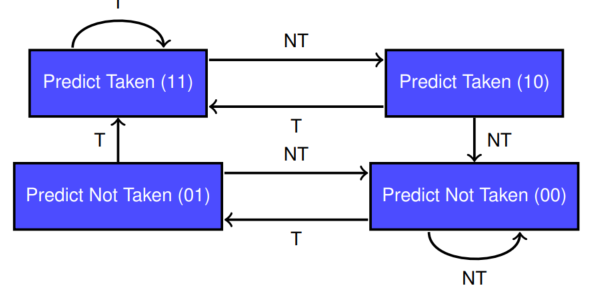
\includegraphics[scale=.4]{Untitled 9.png}}
  \end{figure}

  Funciona esta predicción gracias a la regularidad de los bucles y estructuras de datos.

  Fallan menos que la predicción estática.
\end{itemize}
    
\end{itemize}

\section{Operaciones multiciclo}

\begin{itemize}
\item Las operaciones de coma flotante toman más de un ciclo.
\begin{itemize}
  \item Para que tomaran un solo ciclo, habría que hacerlos más largos, pero eso tendría un impacto negativo global.
  \item Para solventarlo: Segmentación de coma flotante.
  \begin{itemize}
    \item Repetir EX varias veces hasta completarla.
    \item Con su propio pipeline, varias unidades funcionales en EX: Entera, multiplicación FP y Entero, sumador FP, divisor FP y entero.
    \begin{figure}[H]
      \ffigbox[\FBwidth]
      {\caption{Operaciones multiciclo}}
      {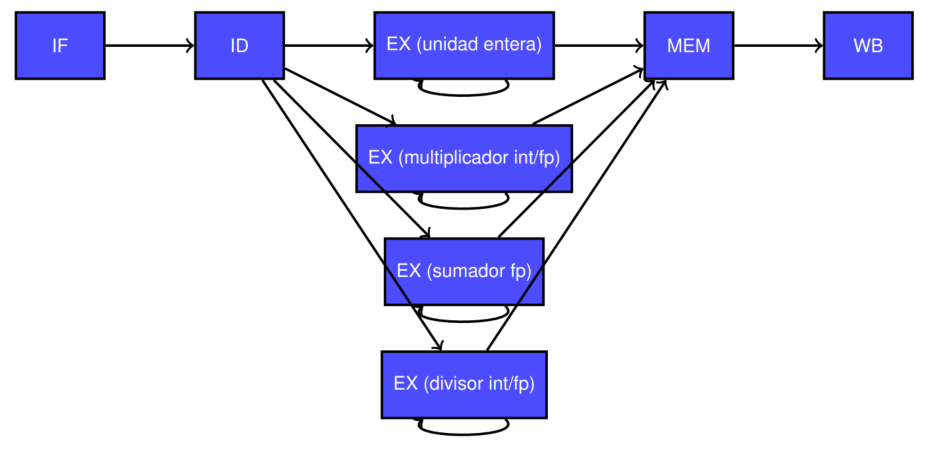
\includegraphics[scale=.4]{Untitled 10.png}}
    \end{figure}
  
  \end{itemize}
      
  \item Latencia: Número de ciclos entre la instrucción que produce un resultado y la instrucción que usa el resultado. Según la dependencia de datos.
  
  \item Intervalo de iniciación: Número de ciclos entre la emisión de dos instrucciones que usan la misma unidad funcional. Depende del uso de unidades funcionales.
\end{itemize}
   

\end{itemize}

\section{Técnicas de compilación e ILP -- Paralelismo a Nivel de
Instrucción}

\begin{itemize}
\item En ILP se aplica a bloques básicos.
    
    - Bloque básico: Secuencia de instrucción sin saltos. En un programa típico MIPS el tamaño de bloque es de 3-6 instrucciones.
\item Aprovechamiento de paralelismo: Entrelazar ejecuciones de instrucciones no relacionadas. Rellenando las detenciones con instrucciones, pero sin alterar resultados.
   
    - El compilador es capaz de optimizarlo, lo pasa ensamblador y lo planifica.
    
    - Planificar: Consiste en reordenar las operaciones para reducir o eliminar latencias(stall)
    
    - Las latencias vienen determinadas por el procesador en su manual.
\item Desenrollamiento de bucles (Loop and rolling)
\begin{itemize}
  \item Consiste en réplica varias veces el cuerpo del bucle y ajustar el código de terminación del bucle. Usa registros distintos para evitar dependencias.
  \item Tratamos de ampliar el tamaño del bloque básico, poniendo varias iteraciones en una solo.
  
      - Desenrollado x4, es poner 4 iteraciones y requiere 4 veces menos vueltas al bucle.
  \item El problema:
  
      - Se requieren más registros.

      - Se debe poder dividir las iteraciones totales entre el factor de desenrollado.
  \item Tras desenrollar podemos planificar para aprovechar los stall, teniendo cuidado con las dependencias.
  
      - 1º Original.

      - 2º Desenrollar.

      - 3º Planificar.
  \item Limitaciones del desenrollamiento de bucles.
  \begin{itemize}
    \item Decremento de la ganancia con cada desenrollamiento.
    
    - Se puede llegar un punto que se eliminen todas las detenciones.
    \item Crecimiento en tamaño de código.
    
    - Puede afectar a que falle la caché.
    \item Presión sobre banco de registros.
    
    - Pueden llegar a faltar registros
  \end{itemize}
      
\end{itemize}
    

\item Límites del ILP 

Procesador ideal

\begin{figure}[H]
	\ffigbox[\FBwidth]
	{\caption{Límites del ILP}}
	{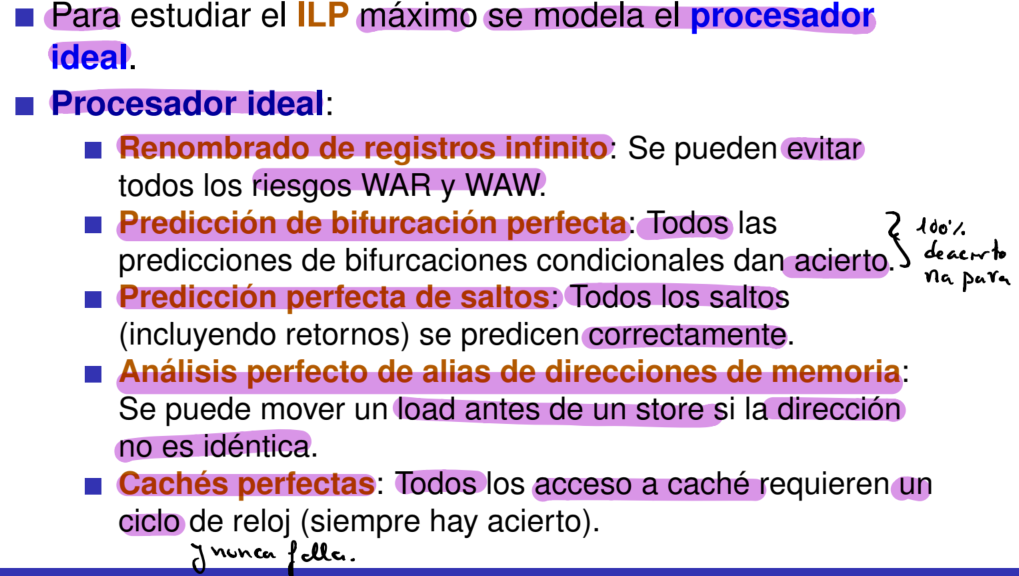
\includegraphics[scale=.3]{Untitled 11.png}}
\end{figure}

  \begin{itemize}
  \item Más ILP implica más lógica de control, más silicio.
       
        - Caches de menor tamaño.

        - Ciclos de reloj más largos.

        - Mayor consumo de energía.
  \item Emisión de 3 a 6 instrucciones por ciclo, a partir de ahí ya no merece invertir más en mejorar el diseño. Se llegó sobre el 2003 a este punto.
  \end{itemize}
\end{itemize}




\section{Técnicas avanzadas de predicción de salto}

\begin{itemize}
  \item Resumen

    \begin{itemize}
    
    \item
      Las bifurcaciones tienen un alto impacto sobre el rendimiento de
      los programas. Hay incertidumbre si el salto se hará o no.
    \item
      Para reducir el impacto:

      \begin{itemize}
      
      \item
        Desenrollamiento de bucles, aumenta el tamaño del bloque básico,
        hay más separación entre branch y se aprovechan los huecos.
      \item
        Predicción de saltos: Estática o Dinámica.

        
          En tiempo de compilación, primero se compila y se reorganiza.

          Comportamiento de cada bifurcación de forma aislada.
      \item
        Predicción avanzada de saltos:

        
          Predictores con correlación.
          
          Predicción por turnos.
        \end{itemize}
      \end{itemize}
  \item Planificación dinámica

    \begin{itemize}
    
    \item
      El hardware reordena la ejecución (no solo lo hace el software) de
      instrucciones para reducir detenciones manteniendo el
      comportamiento de flujo de datos y excepciones.
    \item
      Puede tratar casos no conocidos en tiempo de compilación.

      \begin{itemize}
      
      \item
        Fallos/aciertos en caché, cuando ocurren, ejecutamos
        instrucciones no afectadas.
      \item
        Lo anterior provoca menos dependencia de un pipeline concreto.
        Simplifica el compilador, para una familia de procesadores
        concreta.
      \end{itemize}
    \item
      Permite la especulación hardware.
    \end{itemize}
  \item Predicción con correlación.

    \begin{itemize}
    
    \item
      Cada bifurcación se acuerda de las anteriores bifurcaciones para
      poder elegir entre los predictores.
    \item
      Sugiere que hay correlación entre las bifurcaciones.

      \begin{itemize}
      
      \item
        Si ocurren ciertas bifurcaciones se tomará esta o no.
      \end{itemize}
    \item
      Se almacena la historia de las últimas bifurcaciones para
      seleccionar entre predictores.
    \item
      Un predictor (m, n)

      \begin{itemize}
      
      \item
        El resultado de las m últimas bifurcaciones para seleccionar
        entre \(2^m\) predictores.
      \item
        Cada predictor de n bits.
      \item
        El típico es (1, 2), se acuerda de 1 para elegir entre 2
        predictores.
      \item
        Hay varias entradas por cada dirección de bifurcación.
      \item
        Tamaño total: \(T = 2^m*n*entradas_{dirección}\)
      \end{itemize}
    \item
      Tasa de fallos:

      \begin{itemize}
      
      \item
        Predicción con correlación tiene menos fallos, en general.
      \end{itemize}
    \end{itemize}
  \item Predicción por turnos.

    \begin{itemize}
    
    \item
      Combina dos predictores: Porque no se computa igual los enteros y
      cama flotante

      \begin{itemize}
      
      \item
        Predictor basado en información global.

        \begin{itemize}
        
        \item
          Como uno de correlación de todo el código.
        \end{itemize}
      \item
        Predictor basado en información local.

        \begin{itemize}
        
        \item
          Como Branch History Table, solo se esa Branch.
        \end{itemize}
      \end{itemize}
    \item
      Utiliza un selector para elegir entre predictores.

      \begin{itemize}
      
      \item
        Usa un contador de saturación de 2 bits, parecido a como los usa
        la tabla de histórico de saltos, pero con predicción global y
        local.
      \end{itemize}
    \end{itemize}
  \item Intel Core i7:

    \begin{itemize}
    
    \item
      Predictor de dos niveles:

      \begin{itemize}
      
      \item
        Primer nivel más pequeño, más rápido.
      \item
        Segundo predictor más grande como backup.
      \end{itemize}
    \item
      Cada predictor grande o pequeño tiene 3 predictores:

      \begin{itemize}
      
      \item
        Predictor simple de 2 bits.
      \item
        Predictor de historia global. BHT.
      \item
        Predictor de salida de bucle. Se fija en los bucles cuantas
        veces se va a ejecutar y la próxima vez asume que se ejecuta
        esas veces.
      \end{itemize}
    \item
      Además:
      \begin{itemize}
        \item Predicción de saltos indirectos. En programas que usan Orientados a
          Objetos.
  
        \item Predicción de direcciones de retorno. Predice la dirección del
          que llama/retorno.
      \end{itemize}
    \end{itemize}
  \end{itemize}
  \section{Introducción a la planificación dinámica}

  \begin{itemize}
  
  \item
    El hardware reordena la ejecución de instrucciones para reducir
    detenciones, ejecutando otras mientras no haya dependencias.
  \item
    Ventajas:

    \begin{itemize}
    
    \item
      Código compilado optimizado para un pipeline ejecuta
      eficientemente en otro pipeline.
    \item
      Gestiona dependencias desconocidas en tiempo de compilación, como
      fallos de caché.
    \item
      Permite tolerar retrasos no predecibles.
    \end{itemize}
  \item
    Desventaja: Mayor complejidad del hardware.
  \item
    Efecto:

    \begin{itemize}
    
    \item
      Ejecución fuera de orden, otro orden con respecto al escrito en
      ensamblador.
    \item
      Finalización fuera de orden, cambia el orden de las instrucciones
      y por tanto también su terminación.
    \item
      Puede introducir riesgos WAR y WAW.
    \end{itemize}
  \item
    Separación de etapa ID en dos etapas:

    \begin{itemize}
    
    \item
      Emisión: Coge la instrucción del RI, la decodifica y comprueba
      riesgos estructurales, y si hay hace esperar a la siguiente etapa.
    \item
      Lectura de operandos: Cuando no hay riesgo de datos lee los
      operandos.
    \end{itemize}
  \item
    Etapa de captación IF: Capta 1 instrucción de memoria y la va
    poniendo en un buffer de instrucciones a la cola.

    \begin{itemize}
    
    \item
      Cambia RI por buffer de instrucciones.
    \end{itemize}
  \item
    Técnicas:
  

    \begin{itemize}
      \item
      Scoreboard o Marcador: Detiene instrucciones emitidas hasta que hay
      recursos suficientes y no hay riesgos de datos.
    \item
      Algoritmo de Tomasulo: Elimina dependencias WAR y WAW con
      renombrado de registros.
    \end{itemize}
  \end{itemize}

  \section{Especulación o Ejecución especulativa}

  \begin{itemize}
  
  \item
    Al aumentar el paralelismo conseguido, las dependencias se
    convierten en un problema, cada vez hay más bifurcaciones.
  \item
    Ahora no solo me vale con captar la instrucción, sino que asumo el
    resultado y voy ejecutando instrucciones asumiendo que lo especulado
    es correcto.

    \begin{itemize}
    
    \item
      Se capta, emite y ejecuta instrucciones.
    \item
      Necesitamos un mecanismo de arrepentimiento, para deshacer
      instrucciones cuando no acierta.
    \end{itemize}
  \item
    Ideas:

    \begin{itemize}
    
    \item
      Predicción dinámica de saltos: Selecciona las instrucciones a
      ejecutar.
    \item
      Especulación: ejecución antes de que se resuelvan dependencias de
      control, con capacidad de deshacer.
    \item
      Planificación dinámica.
    \end{itemize}
  \item
    Para conseguirlo se debe separar el paso del resultado entre
    instrucciones y la finalización de la instrucción. No se actualiza
    el estado de los registros y memoria hasta que hay confirmación.

    \begin{itemize}
    
    \item
      Para eso se usa: ROB -- Reorder Buffer -- Buffer de reordenamiento

      \begin{itemize}
      
      \item
        Es un array de 4 columnas fundamental para la especulación,
        entradas:

        \begin{itemize}
        
        \item
          Tipo de instrucción.
        \item
          Destino: Id de registro o dirección de memoria.
        \item
          Valor del resultado.
        \item
          Ready: Si se ha completado la instrucción.
        \end{itemize}
        \item
      Cuando se finaliza una instrucción se escribe en el ROB, y cuando
      se confirma se escribe en el destino real y si no se descartan.
      
      \item
        Las siguientes instrucciones leen del ROB.
      \end{itemize}
    
    \end{itemize}
  \end{itemize}
\newpage
  \section{Técnicas de emisión múltiple}

  \begin{itemize}
  
  \item
    Consiste en conseguir un CPI menor de 1, se puede iniciar más de una
    instrucción por ciclo.
  \item
    Procesador superescalar, son lo que pueden hacer emisión múltiple.

    \begin{itemize}
    
    \item
      Procesadores superescalares planificados estáticamente:

      \begin{itemize}
      
      \item
        Emisión: Dinámica, no cogen siempre el mismo número de
        instrucciones.
      \item
        Detección de riesgos: Hardware.
      \item
        Planificación: Estática.
      \item
        Lo que le diferencia: Ejecutan las instrucciones en orden.
      \end{itemize}
    \item
      Procesadores superescalares planificados dinámicamente:

      \begin{itemize}
      
      \item
        Sin especular:

        \begin{itemize}
        
        \item
          Emisión: Dinámica.
        \item
          Detección de riesgos: Hardware.
        \item
          Planificación: Dinámica.
        \item
          Lo que le diferencia: Ejecutan fuera de orden, cambian el
          orden para aprovechar el procesador.
        \item
          NO hay ninguno que no especule.
        \end{itemize}
      \item
        Especulativo:

        \begin{itemize}
        
        \item
          Emisión: Dinámica.
        \item
          Detección de riesgos: Hardware.
        \item
          Planificación: Dinámica con especulación.
        \item
          Lo que le diferencia: Ejecutan fuera de orden con
          especulación.
        \end{itemize}
      \end{itemize}
    \item
      Procesadores VLIW -- Palabra de Instrucción Muy Larga.

      \begin{itemize}
      
      \item
        Varias instrucciones empaquetadas.
      \item
        Planifica estáticamente, en orden.
      \item
        ILP por el compilador.
      \item
        El código debe presentar suficiente paralelismo como para que
        pueda usar todas las instrucciones.
      \item
        El programador es el responsable de crear el paquete con
        instrucción compatible, el compilador casi siempre los crea de
        una sola y no merece la pena.
      \item
        Emisión: Estática.
      \item
        Detección de riesgos: Software.
      \item
        Planificación: Estática.
      \item
        Lo que le diferencia: Riesgos determinado e indicado por el
        compilador (software).
      \item
        Desventajas:

        \begin{itemize}
        
        \item
          Complejidad de encontrar paralelismo estáticamente.
        \item
          Tamaño del código generado, demasiado grande.
        \item
          No tiene hardware de detención de riesgos.
        \item
          Problemas de compatibilidad binaria mayores que en
          superescalares.
        \end{itemize}
      \end{itemize}
    \item
      EPIC: Mejora el VLIW

      \begin{itemize}
      
      \item
        Emisión: Principalmente estática.
      \item
        Detección de riesgos: Principalmente software.
      \end{itemize}
    \item
      Planificación: Sobre todo estática.

      \begin{itemize}
      
      \item
        Lo que le diferencia: Riesgos determinado e indicado por le
        compilador (software)
      \end{itemize}
    \end{itemize}
  \end{itemize}

 \section{Paralelismo a nivel de hilo -- TLP}

    Algunas aplicaciones presentan más paralelismo natural, que
    claramente su función lo necesita o se beneficia mucho de este.

    Dos modelos:
\subsection{Paralelismo a nivel de Hilos -- TLP}

      \begin{itemize}
        \item
          Hilo: Proceso con sus propias instrucciones y datos.
        \item
          Pueden ser parte del programa o independientes.
        \item
          Cada hilo tiene su propio estado (instrucciones, datos, PC,
          registros, \ldots)

          \begin{itemize}
          
            \item
              Múltiples hilos de ejecución paralelos.
            \item
              Mejor tasa de procesamiento cuando se ejecutan muchos
              programas.
            \item
              Mejor tiempo de ejecución de programas multihilo.
          \end{itemize}
        \item
          Ejecución multihilo: Múltiples hilos comparten las unidades
          funcionales de un procesador.

          \begin{itemize}
          
            \item
            Necesita replicar n veces el estado, según el número de hilos.

            \item
            Tipos: Según cada cuantos ciclos cambia de hilo. 
            \begin{itemize}
              \item Resumen
              \begin{figure}[H]
                \ffigbox[\FBwidth]
                {\caption{Paralelismo a nivel de Hilos}}
                {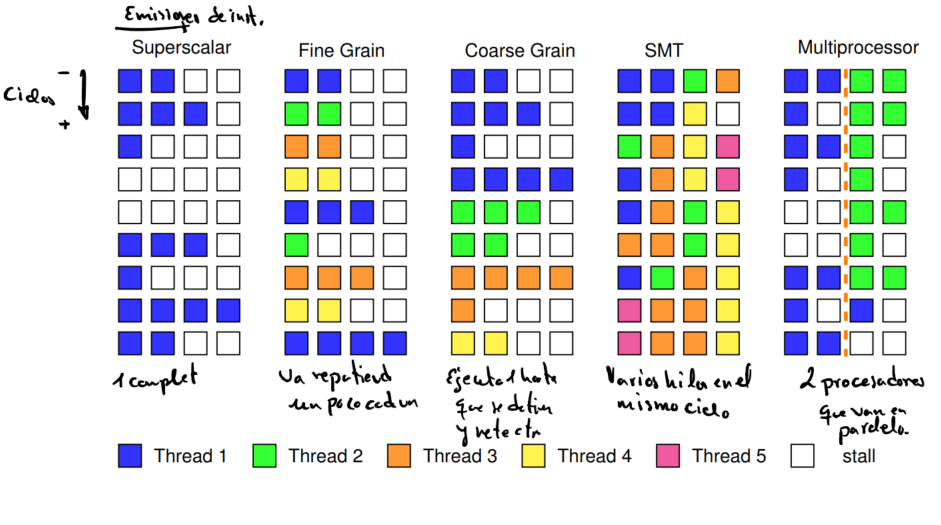
\includegraphics[scale=.3]{Untitled 12.png}}
              \end{figure}
              \item Grano fino: Alterna cada ciclo de hilo, saltado las detenciones.
              \begin{itemize}
                \item Entrelaza la ejecución de los hilos.
                \item Normalmente round-robin, menos las detenciones.
                \item Ventaja: Oculta detenciones cortas y largas.
                \item Desventaja: Retrasa la ejecución de hilos individuales.
              \end{itemize}
                  
              \item Grano grueso: Cambia de hilo solo en detenciones largas.
              \begin{itemize}
                \item Ventajas:
                
                - No hace falta cambio de hilo demasiado rápido.

                - No retrasa hilos individuales.
                \item Desventajas:
                
                - Se debe vacía o congelar el pipeline.

                - Se debe llenar el pipeline con instrucciones del nuevo hilo.
                \item Cuando llenar el pipeline es más corto que la detención.
              \end{itemize}
                  
              \item Multi-hilo simultáneo (Hyperthreading): En un núcleo puede tratar varias instrucciones por ciclo.
              \begin{itemize}
                \item Procesadores con planificación dinámica ya tienen muchos mecanismos de soporte para multi-hilo.
                
                - Grandes conjuntos de registros virtuales.

                - Renombrado de registros.

                - Finalización fuera de orden.
                \item Modificaciones:
                
                - Tabla de renombrado por hilo

                - Registros PC separados.

                - ROB separado.
              \end{itemize}
                  
            \end{itemize}
          \end{itemize}
      \end{itemize}
      \subsection{Paralelismo a nivel de Datos -- DLP}
          Operaciones idénticas sobre distintos datos.
  
  \chapter{Módulo 4 Jerarquía de memoria}
  \section{Evolución de la latencia}

    \begin{itemize}
    
    \item
      Múltiples visiones del rendimiento,
      \(Rendimiento =\frac 1 {latencia}= \frac 1 {tiempo\space desde\space que\space se\space inicia\space hasta\space que\space termina}\).
      Para evaluar procesadores y memoria.
    \item
      Procesadores: Desde que comienza hasta que termina una operación.

      \begin{itemize}
      
      \item
        Incremento anual del rendimiento: 25\% y 52\%.
      \item
        Efecto combinado de 1980 a 2010, superior a 3000 veces.
      \end{itemize}
    \item
      Memoria: Desde que comienza la lectura o escritura hasta que
      termina.

      \begin{itemize}
      
      \item
        Incremento anual del rendimiento: 7\%.
      \item
        Efecto combinado de 1980 a 2010, superior a 7.5 veces.
      \end{itemize}
    \end{itemize}

    Se ha mejorado mucho más el rendimiento del procesador que el de
    memoria, lo que provoca el Muro de Memoria, lo que hace lento la
    ejecución es el tiempo en acceder a memoria.
  
    \section{Efecto multi-core}
    \begin{figure}[H]
      \ffigbox[\FBwidth]
      {\caption{Efecto multi-core}}
      {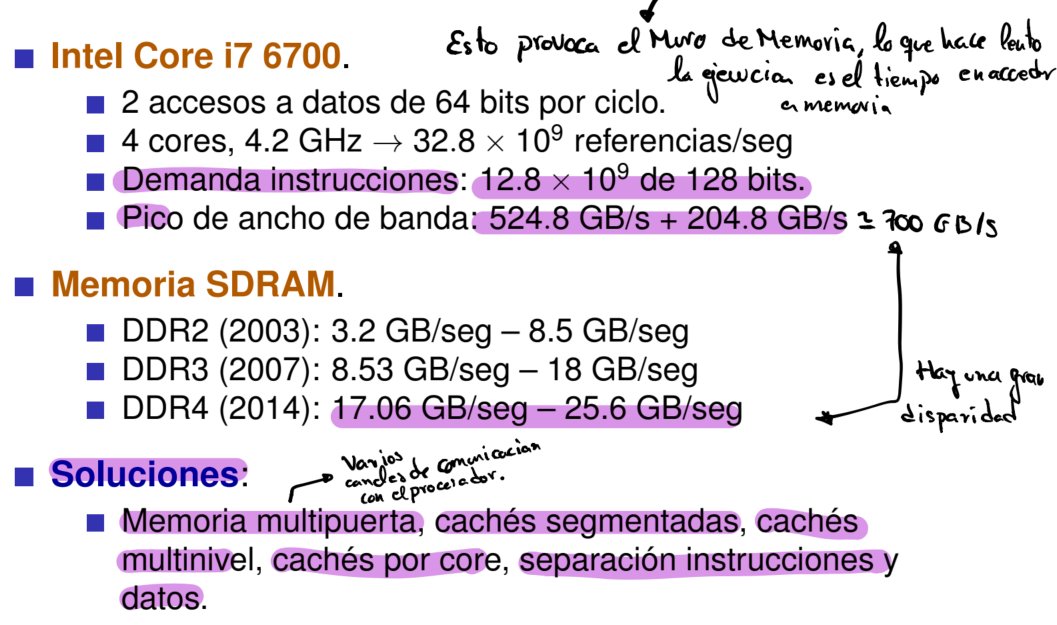
\includegraphics[scale=.4]{Untitled 13.png}}
    \end{figure}
  \section{Principio de localidad}
     Es una propiedad de los algoritmos, no del
    hardware, pero lo aprovecha. Los programas acceden una porción
    relativamente pequeña del espacio de direcciones.

    \begin{itemize}
    
    \item
      Se trata de tener los datos cercanos para acceder rápido, ya que
      sabemos que es posible que lo accedamos.
    \item
      Tipos de localidad: Visiones complementarias.

      \begin{itemize}
      
      \item
        Localidad temporal: Los elementos accedidos recientemente
        tienden a volver a ser accedidos.
      \item
        Localidad espacial: Los elementos próximos a los accedidos
        recientemente tienden a ser accedidos.
      \end{itemize}
    \end{itemize}
  \section{Situación (2018)}
    \begin{figure}[H]
      \ffigbox[\FBwidth]
      {\caption{Situación 2018 memorias}}
      {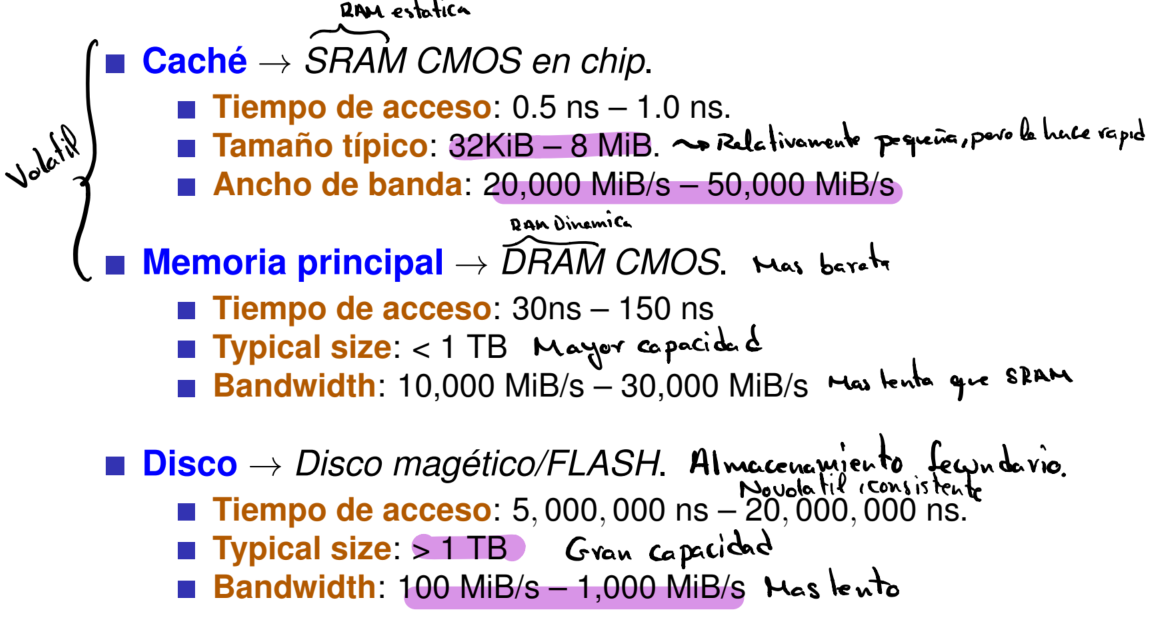
\includegraphics[scale=.35]{Untitled 14.png}}
    \end{figure}
    \pagebreak
  \section{Jerarquía de memoria}

    \begin{itemize}
    
    \item
      De menor a mayor capacidad, de más rápida a más lenta. Si está el
      dato, acierto, lo pasa al procesador y si no, fallo, lo pedimos a
      la caché superior.

      \begin{itemize}
      
      \item
        Procesador
      \item
        Cache L1: Del orden del kB.
      \item
        Caché L2
      \item
        Caché L3
      \item
        Memoria principal.
      \end{itemize}
    \item
      Bloque o línea: Unidad de copia. Formada por múltiples palabras,
      es un parámetro del hardware. En Intel 64 bytes.
    \item
      Acierto: El dato accedido está presente en el nivel superior.

      \begin{itemize}
      
      \item
        Tasa de aciertos = \(h= \frac {aciertos} {accesos}\)
      \end{itemize}
    \item
      Fallo: Si el dato accedido está ausente.

      \begin{itemize}
      
      \item
        Penalización de fallo: Tiempo en resolver el fallo.
      \item
        Tasa de fallo = \(m= \frac {fallos} {accesos}=1-h\)
      \end{itemize}
    \end{itemize}
  \section{Medidas}

    \begin{itemize}
    
    \item
      Tiempo medio de acceso a memoria: \(t_M=t_A+(1-h)t_F\)

      \begin{itemize}
      
      \item
        \(t_A\): Tiempo de acceso.
      \item
        \(t_F\): Tiempo de fallo.
      \end{itemize}
    \item
      Penalización de fallo: Tiempo en remplazar bloque y entregarlo a
      CPU.
    \item
      Tiempo de acceso: Tiempo de obtenerlo de nivel inferior.
    \item
      Tiempo de transferencia: Tiempo de transferir un bloque.
    \item
      Tiempo de ejecución de CPU:
      \(t_{CPU}=(ciclos_{CPU}+ciclos_{detencionMemoria})*t_{ciclo}\)
    \item
      Ciclos de reloj CPU: \(ciclos_{CPU}=IC*CPI\)
    \item
      Ciclos de detención de memoria:
      \(ciclos_{detención\space memoria}= n_{fallos}*penalización_{fallo}= IC*fallo_{instr}*penalización_{fallo}= IC*accesos\_memoria_{instr}*(1-h)*penalización_{fallo}\)
    \end{itemize}
  \section{Políticas y estrategias}

    \begin{itemize}
    
    \item
      Políticas:

      \begin{itemize}
      
      \item
        Ubicación de bloque: donde se ubica un bloque.

        \begin{itemize}
        
        \item
          Correspondencia directa: Hay un único lugar donde se coloca,
          se asigna de forma cíclica.

          
            Ubicación: bloque mod \(n_{bloque}\)

            \item
          Correspondencia totalmente asociativa: Pueden ocupar cualquier
          lugar, se almacenan pares claves y valor.
        \item
          Correspondencia asociativa por conjuntos: Equilibrio de los
          anteriores. Los bloques tienen asignado un conjunto, y dentro
          puede estar en cualquier hueco.

          
            Ubicación de conjunto: bloque mod \(n_{conjuntos}\)

          \end{itemize}
      \item
        Identificación de bloque: Como se localiza un bloque.

        \begin{itemize}
        
        \item
          Hay varios campos: Etiqueta \textbar{} Índice \textbar{}
          Desplazamiento. Se toman x bits si el tamaño es \(2^x\) bytes.

          \begin{itemize}
          
          \item Dirección de bloque: Encontrar el bloque.

              Etiqueta: Identifica la dirección en entrada.

              Índice: Selecciona el conjunto.

          \item Desplazamiento de bloque: Selecciona el dato dentro del
            bloque. Offset.
          \end{itemize}
        \item
          Con mayor asociatividad:

          Menos bit de índice.

          Más bits de etiqueta.

        \end{itemize}
      \item
        Remplazo de bloque: Que bloque debe remplazarse.

        \begin{itemize}
        
        \item
          Relevante para asociativa y asociativa por conjuntos, no para
          directa, ya que hay un único candidato para echar:

          \begin{itemize}
          
          \item
            Aleatorio: Fácil de implementar.
          \item
            LRU: Menor recientemente usado. Complejidad creciente.
          \item
            FIFO: El primero en entrar, el primero en salir. Puede ser
            peor que LRU, pero es menos complejo que LRU.
          \end{itemize}
        \item
          LRU y FIFO son mejor que aleatorio.
        \end{itemize}
        \pagebreak
      \item
        Estrategia de escritura: Que se debe hacer cuando modificamos un
        dato.

        \begin{itemize}
        \item
          Escritura inmediata -- write-through: Las escrituras van a
          caché y memoria inmediatamente. Fácil de implementar, aunque
          puede haber problema si todos lo realizan a la vez.
        \item
          Post-escritura -- write-back: Solo escribe cuando van a ser
          expulsado de caché. Problema de propagación y serialización.
          Más complejo.

          \begin{figure}[H]
          \ffigbox[\FBwidth]
          {\caption{Estrategias de escritura}}
          {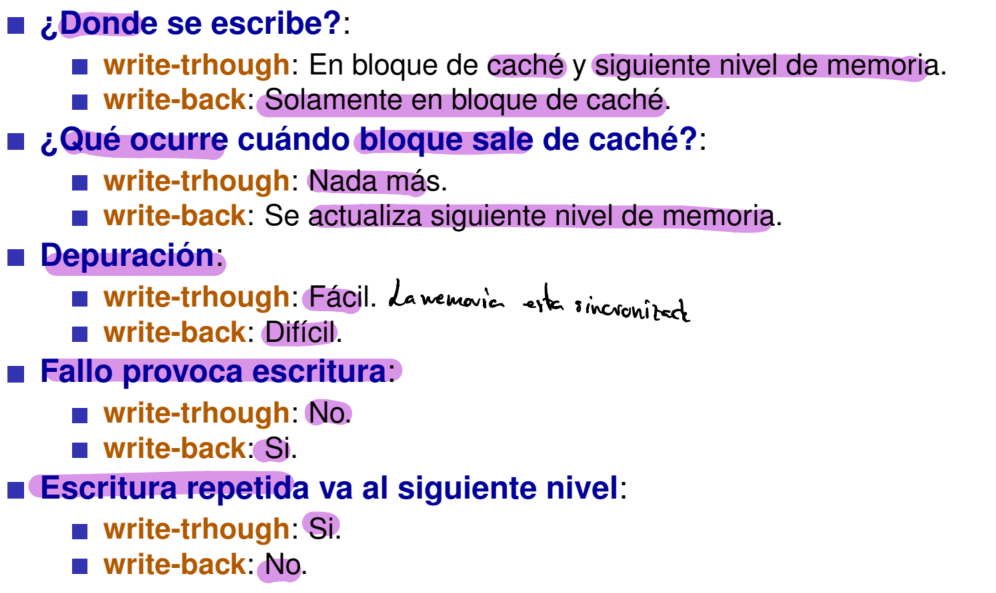
\includegraphics[scale=.3]{Untitled 15.png}}
        \end{figure}
        \end{itemize}
      \end{itemize}
    \item
      Penalización de fallo: Latencia total del fallo y Latencia
      expuesta, cuanto tiene que parar la CPU.
      $$\frac {ciclos\_detencion_{memoria}} {IC}= \frac {fallos} {IC}*(latencia_{total}-latencia_{solapada})$$
    \end{itemize}
  \section{Buffer/Cola de escritura}

    \begin{itemize}
    
    \item
      Cuando va a modificar un dato lo escribe en el buffer, se da por
      completada la escritura en memoria.

      \begin{itemize}
      
      \item
        En escritura inmediata, se escribe en el buffer cada vez.
      \item
        En escritura retrasada, se usa solo cuando se saca el bloque de
        caché.
      \end{itemize}
    \item
      También permite que si se reciben varias peticiones de escritura
      de posiciones próximas agruparlas para hacer una única escritura
      en memoria.
    \item
      Buffer al lado de la caché donde se almacenan valores para la
      memoria principal, mientras otra instrucción la está usando, de
      esta manera podemos seguir ejecutando y otros mecanismos llevaron
      más tarde lo del buffer a la memoria principal.
    \end{itemize}
  \section{Tasa de fallos global y local}
  \begin{figure}[H]
    \ffigbox[\FBwidth]
    {\caption{Tasa de fallos global y local}}
    {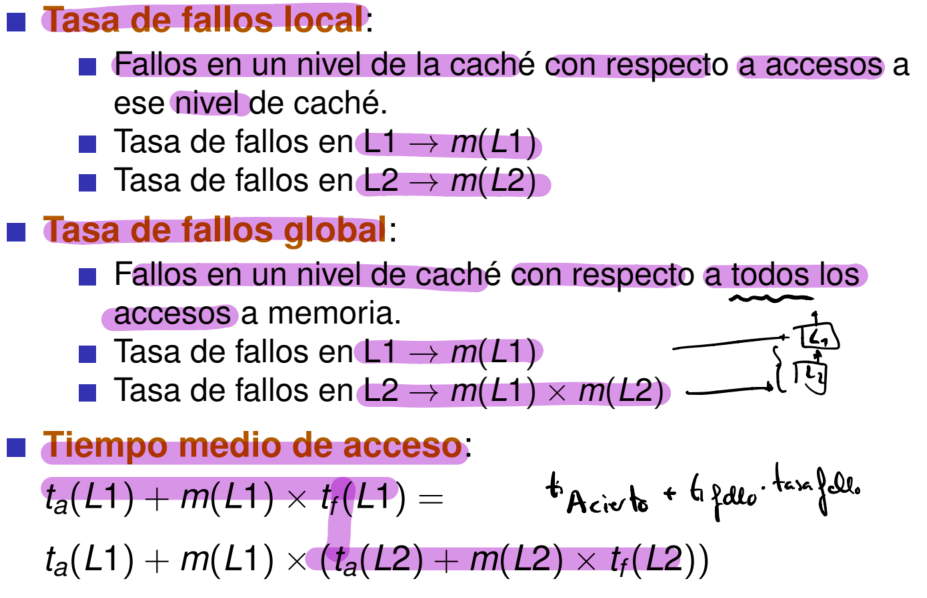
\includegraphics[scale=.4]{Untitled 16.png}}
  \end{figure}
  \begin{figure}[H]
    \ffigbox[\FBwidth]
    {\caption{Tasa de fallos global y local}}
    {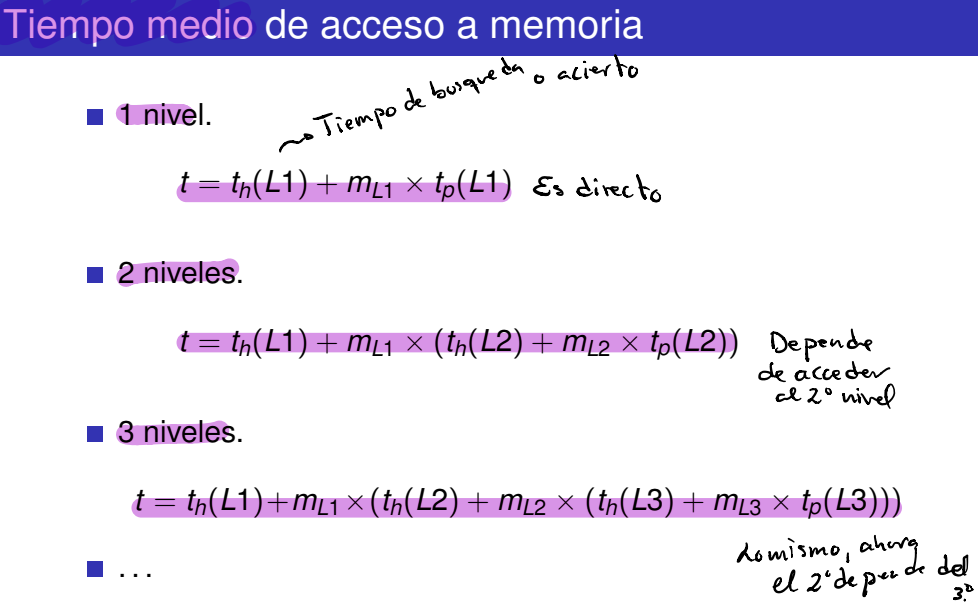
\includegraphics[scale=.4]{Untitled 17.png}}
  \end{figure}
  \section{Optimizaciones básica de cache:}

  Dirigidas a mejorar la velocidad de acceso.

  \subsection{Reducción de tasa de fallos}

  \begin{itemize}
  
  \item
    Aumentar de tamaño de bloques:

    \begin{itemize}
    
    \item
      Mejor aprovechamiento de localidad espacial. Caben más datos por
      bloque. Menos bloques por caché.
    \item
      Menor la tasa de fallos.
    \item
      Mayor penalización por fallo, hay que mover más datos.
    \item
      Necesidad de equilibrio: Buscar el punto óptimo de tamaño, 64
      bytes.

      \begin{itemize}
      
      \item
        Alta latencia y alto ancho de banda, incrementar tamaño de
        bloque.
      \item
        Baja latencia y bajo ancho de banda, tamaño de bloque reducido.
      \end{itemize}
    \end{itemize}
  \item
    Aumentar de tamaño de caché:

    \begin{itemize}
    
    \item
      Menor tasa de fallos.
    \item
      Más datos en la caché, caben más bloques.
    \item
      Tarda más en buscar en caché.
    \item
      Mayor coste y consumo de energía.
    \end{itemize}
  \item
    Incrementar de asociatividad:

    \begin{itemize}
    
    \item
      Menor tasa de fallos. Menos conflictos.
    \item
      Al haber más vías es más difícil que haya que dejar 1.
    \item
      Puede incrementar tiempo de acierto, tarda más en buscar.
    \item
      Totalmente asociativo, aprox. 8 vías. Poner más deja de mejorar.
    \end{itemize}
  \end{itemize}

\subsection{Reducción de penalización de fallos}

  \begin{itemize}
  
  \item
    Introducir caches multinivel:

    \begin{itemize}
    
    \item
      Reducción de la penalización de fallos.
    \item
      Evolución: Mayor distancia entre rendimiento de DRAM y CPU. Coste
      de penalización de fallo creciente.
    \item
      Alternativas: Hacer la caché más rápida y más grande.
    \item
      Solución: Hacer las dos cosas y varios niveles de caché.
    \end{itemize}
    \pagebreak
  \item
    Dar prioridad de fallos de lectura sobre escrituras:

    \begin{itemize}
    
    \item
      Reduce la penalización de fallos. Evita que un fallo de lectura
      tenga que esperar a que una escritura termina.
    \item
      Caches de escritura inmediata: El buffer de escritura podría
      contener una modificación del fato que se lee. Buffer al lado de
      caché donde se escriben los valores a memoria principal

      \begin{itemize}
      \item
        \begin{enumerate}
        \def\labelenumi{\alph{enumi})}
        
        \item
          Esperar el vaciado del buffer de escritura y otro mecanismo
          los copiará más tarde en memoria principal.
        \end{enumerate}
      \item
        \begin{enumerate}
        \def\labelenumi{\alph{enumi})}
        \setcounter{enumi}{1}
        
        \item
          Comprobar los valores del buffer de escritura.
        \end{enumerate}
      \end{itemize}
    \item
      Caches con post-escritura: Un fallo de lectura podría remplazar un
      bloque modificado.

      \begin{itemize}
      
      \item
        Copiar bloque modificado a buffer.
      \item
        Aplicar opciones a o b.
      \end{itemize}
    \end{itemize}
  \end{itemize}

 \subsection{Reducción de tiempo de acierto}

  \begin{itemize}
  
  \item
    Evitar traducción de direcciones en indexación en caché:
  \end{itemize}

  \section{Optimizaciones avanzadas}

    Trata de reducir: Tiempo de búsqueda, tasa de fallos y penalización
    de fallos.

    Trata de aumentar: Ancho de banda de caché.

   \subsection{Caches pequeñas}

    \begin{itemize}
    
    \item
      El tiempo de búsqueda se incrementa con el tamaño de la caché.
    \item
      Por lo tanto, una más pequeña, hace el hardware de búsqueda más
      simple y cabe en el chip del procesador.
    \item
      Mejora el tiempo de búsqueda.
    \end{itemize}

    \subsection{Caches simples}

    \begin{itemize}
    
    \item
      Mecanismo de correspondencia lo más sencillo posible.
    \item
      La más sencilla es la correspondencia directa, ya que permite
      paralelizar la comparación de etiquetas con la transmisión del
      dato.
    \item
      Caché pequeña es mejor que cache simple.
    \end{itemize}
  \subsection{Predicción de vía:}

    \begin{itemize}
    
    \item
      El problema es:

      \begin{itemize}
      
      \item
        La correspondencia directa es rápida, pero produce muchos
        fallos.
      \item
        La correspondencia asociativa por conjuntos tiene menos fallos,
        pero es más lenta.
      \end{itemize}
    \item
      Almacena bits adicionales para predecir la vía en el próximo
      acceso.
    \item
      Acceso adelantado al bloque y comparación con una única etiqueta,
      si falla se comparan el resto.
    \end{itemize}
  \subsection{Acceso segmentado a la cache:}

    \begin{itemize}
    
    \item
      Trata de aumentar el ancho de banda.
    \item
      Para ello segmenta el acceso a la caché en varios ciclos de reloj.
    \item
      Efectos:

      \begin{itemize}
      
      \item
        Se puede reducir el ciclo de reloj.
      \item
        Se puede iniciar un acceso en cada ciclo de reloj.
      \item
        Se mejora el ancho de banda de la caché.
      \item
        Se aumenta la latencia.
      \end{itemize}
    \item
      Efecto positivo en procesadores superescalares.
    \end{itemize}
  \subsection{Caches no bloqueantes}

    \begin{itemize}
    
    \item
      Problema: Los fallos de caché generan paradas hasta que se recibe
      el bloque.
    \item
      Para evitar paradas, se hace ejecución fuera de orden, que la
      siguiente instrucción en ejecución pueda seguir progresando.
    \item
      Si la siguiente accede a memoria:

      \begin{itemize}
      
      \item
        Acierto durante el fallo: Permite accesos con acierto mientras
        se espera al bloque. Reduce la penalización del fallo.
      \item
        Acierto durante el fallo/ Fallo durante fallo: Permite fallos
        solapados. Necesita memoria multicanal. Es altamente complejo,
        por lo tanto, más probable el fallo.
      \end{itemize}
    \end{itemize}
  \subsection{Caches multi-banco}

    \begin{itemize}
    
    \item
      Busca poder acceder simultáneamente a distintas posiciones de la
      caché.
    \item
      Para ello se divide la memoria en bancos independientes, que se
      pueden acceder simultáneamente por separado, pero no varios en el
      mismo banco.
    \item
      Hay que distribuir los accesos entre los bancos para ver mejora.
      El esquema sencillo es entrelazarlo secuencialmente, los bloques
      se reparten equitativamente (banco1 0 y 2, banco2 1 y 3).
    \item
      Aumenta el ancho de banda.
    \end{itemize}
  \subsection{Palabra critica primero y reinicio temprano}

    \begin{itemize}
    
    \item
      Se basa en que el procesador normalmente necesita una única
      palabra para poder proseguir.
    \item
      La solución es no esperar a recibir el bloque completo, cuando se
      recibe la palabra crítica y se continúa mientras sigue trayendo el
      bloque.
    \item
      Alternativas:

      \begin{itemize}
      
      \item
        Palabra crítica primero: El bloque se recibe reordenado con la
        palabra que necesita el procesador al principio, de esta manera
        no tiene que esperar tanto para continuar.
      \item
        Reinicio temprano: El bloque se recibe sin reordenar, pero
        cuando se recibe prosigue.
      \end{itemize}
    \item
      En la práctica se combinan ambas.
    \item
      Cuanto más grande es el bloque más se aprovecha.
    \end{itemize}
  \subsection{Mezcla en búfer de escritura}

    \begin{itemize}
    
    \item
      Si el búfer contiene bloques modificados, se comprueban las
      direcciones para ver si se pueden sobrescribir, de esta manera no
      se hacen dos escrituras para el mismo bloque.
    \item
      Además, si tenemos varios datos próximos podemos agrupar
      escrituras para hacer una única escritura.
    \item
      Efectos:

      \begin{itemize}
      
      \item
        Reduce el número de escrituras en memoria.
      \item
        Reduce paradas debidas a que el buffer este lleno.
      \end{itemize}
    \end{itemize}
  \subsection{Optimización del compilador}

    \begin{itemize}
    
    \item
      El objetivo es generar código que provoque menos fallos de
      instrucciones y datos.
    \item
      Instrucciones:

      \begin{itemize}
      
      \item
        Reordenamiento de procesamientos.

        \begin{itemize}
        
        \item
          Trata de reducir los fallos por conflicto debidos a que dos
          procesamientos coincidentes en el tiempo se corresponden con
          la misma línea de caché (expulsa).
        \item
          La técnica es reordenar los procedimientos o subrutinas en
          memoria, para evitar que se tenga que expulsar algún
          procedimiento que vamos a volver a usar.
        \item
          Se realiza en tiempo de compilación.
        \end{itemize}
      \item
        Alinear bloques de código al inicio de bloques de caché.

        \begin{itemize}
        
        \item
          Objetivo: Reducir la posibilidad de fallos de caché para
          código secuencial, un bloque básico.
        \item
          Técnica: Hacer coincidir la primera instrucción del bloque
          básico con la primera palabra del bloque.

          
          
            Maximizar el número de instrucciones de la línea, trata de
            reducir fallos.

          \end{itemize}
      \item
        Linealización de saltos:

        \begin{itemize}
        
        \item
          Objetivo: Reducir los fallos de caché debidos a saltos
          condicionales.
        \item
          Técnicas: Si el compilador sabe que es probable que se tome un
          salto, puede cambiar el sentido de la condición en
          intercambiar los bloques básicos de las dos alternativas.
        \end{itemize}
      \end{itemize}
    \item
      Datos:

      \begin{itemize}
      \item
        Fusión de arrays.

        \begin{itemize}
        
        \item
          Reduce los conflictos.
        \item
          Mejora de localidad espacial, cuando se fusiona están
          contiguos los valores con mismo índice, así no hay conflicto
          porque estén lejos.
        \end{itemize}
      \item
        Intercambio de bucles.

        \begin{itemize}
        
        \item
          Trata de mejorar la localidad espacial, cambiando el interno a
          externo o al revés.
        \item
          Depende del modelo de almacenamiento vinculado al lenguaje de
          programación.
        \end{itemize}
      \item
        Fusión de bucles.

        \begin{itemize}
        
        \item
          Objetivo: Mejorar localidad temporal.
        \item
          El fusionado será mejor o igual, pero no peor. ¿?
        \item
          Necesitan el mismo número de iteración.
        \item
          Cuidado: Puede reducir localidad espacial
        \end{itemize}
      \item
        Acceso por bloques

        \begin{itemize}
        
        \item
          Aumenta la tasa de aciertos
        \item
          Consiste en dividir productos matriciales en bloques más
          pequeños.
        \end{itemize}
      \end{itemize}
    \end{itemize}
  \section{Lectura adelantada hardware - Instruction prefetching}

    \begin{itemize}
    
    \item
      Se parte de que las instrucciones presentan alta localidad
      espacial.
    \item
      Lectura de dos bloques en caso de fallo, el que provoca el fallo y
      el bloque siguiente.
    \item
      Ubicación:

      \begin{itemize}
      
      \item
        Bloque que falla, cache de instrucción.
      \item
        Bloque siguiente, búfer de instrucciones y se trae
        posteriormente.
      \end{itemize}
    \item
      Ejemplo: Pentium 4, permite lectura adelantada de páginas de 4 kB a
      caché L2.

      \begin{itemize}
      
      \item
        Se invoca si: 2 fallos en L2 debidos a una misma página.
        Distancia entre fallos menor de 256 bytes.
      \end{itemize}
    \end{itemize}
    \pagebreak
  \subsection{Resumen}
  \begin{figure}[H]
    \ffigbox[\FBwidth]
    {\caption{Optimizaciones avanzadas I}}
    {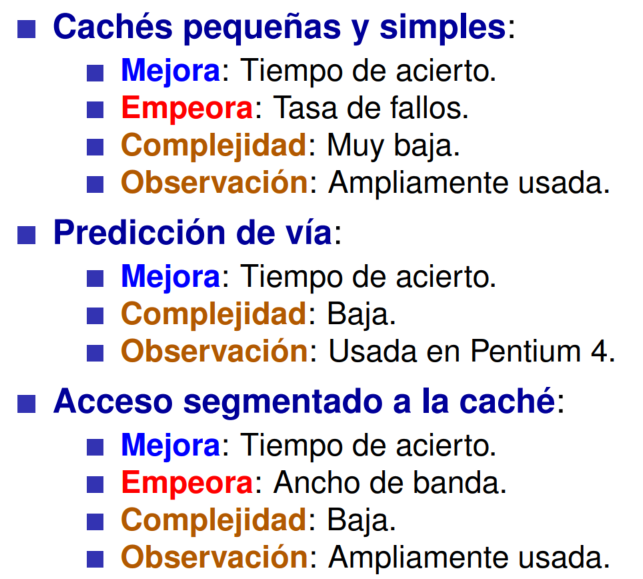
\includegraphics[scale=.35]{Untitled 23.png}}
  \end{figure}
  \begin{figure}[H]
    \ffigbox[\FBwidth]
    {\caption{Optimizaciones avanzadas II}}
    {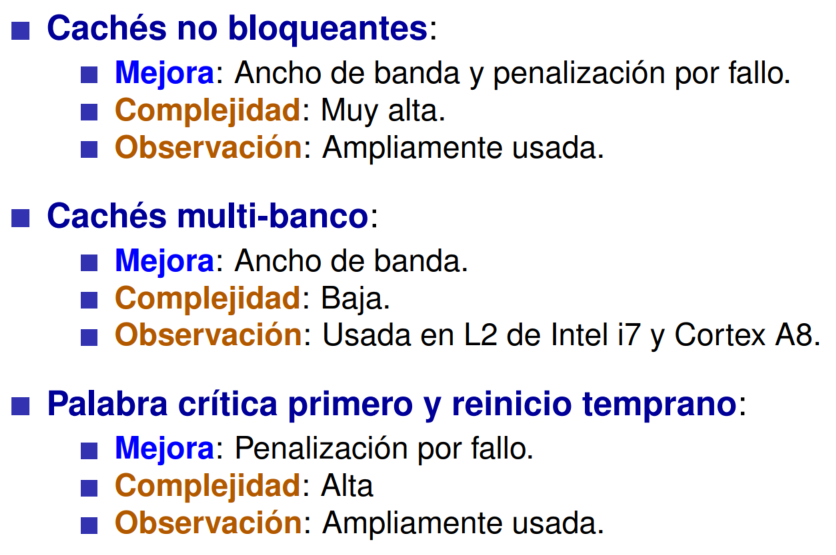
\includegraphics[scale=.3]{Untitled 24.png}}
  \end{figure} 
  \begin{figure}[H]
    \ffigbox[\FBwidth]
    {\caption{Optimizaciones avanzadas III}}
    {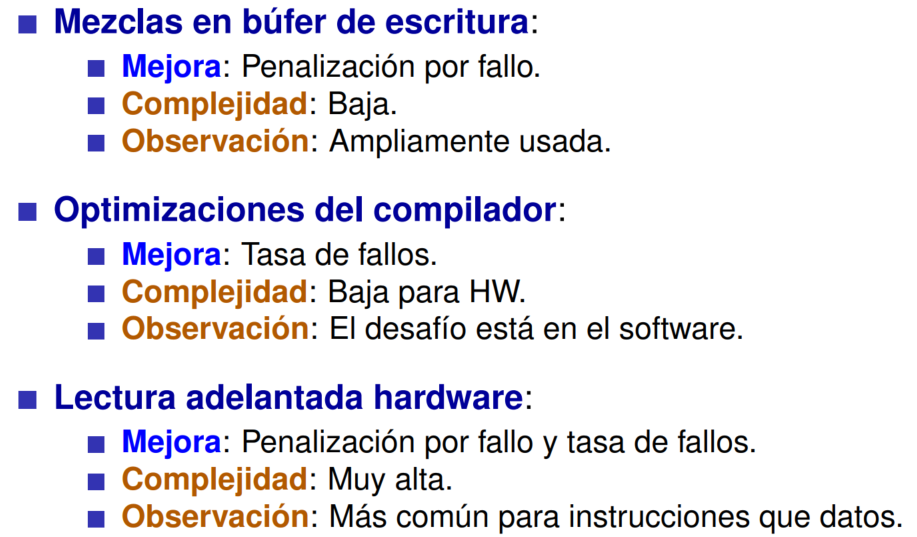
\includegraphics[scale=.3]{Untitled 25.png}}
  \end{figure}


\section{Memoria virtual}
\begin{figure}[H]
	\ffigbox[\FBwidth]
	{\caption{Memoria virtual}}
	{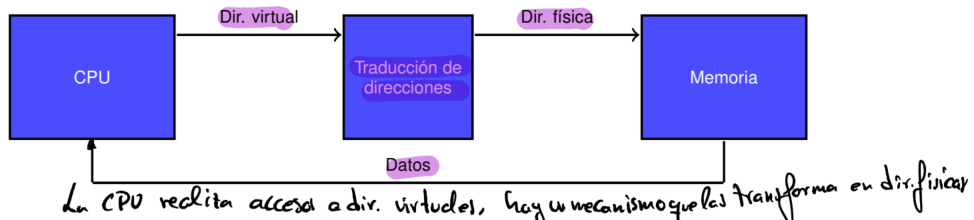
\includegraphics[scale=.4]{Untitled 26.png}}
\end{figure}


    Surge al encontrar límites en la memoria que podemos tener.

  \subsection{Direccionamiento físico}
  \begin{figure}[H]
    \ffigbox[\FBwidth]
    {\caption{Direccionamiento físico}}
    {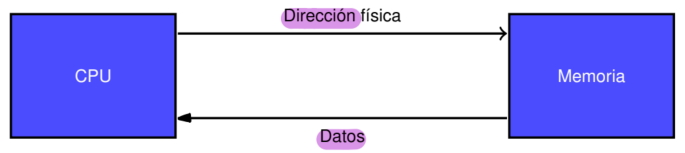
\includegraphics[scale=.4]{Untitled 27.png}}
  \end{figure}
  \begin{itemize}
    \item Todos los datos están en el mismo lugar, cualquier programa que ejecuta en la CPU puede acceder a cualquier dirección de memoria.
    \item
    No hay una manera de evitar que acceda a datos de otro programa.
  \end{itemize}

  La CPU realiza accesos a direcciones del espacio de direcciones
  virtuales normalizadas, detrás hay un mecanismo que las transforma
  en direcciones físicas mediante una tabla.

  \begin{itemize}    
  \item
    Normalizadas: Porque se puede asumir que empiezan en 0, el mecanismo
    los colocará en su sitio en la memoria física.
    
    \item
      La traducción la realiza el hardware, el software sería demasiado
      lento.
    \item
      Lo gestiona el SO.
  \end{itemize}

  Página: Cada uno de los bloques de memoria en lo que se divide un
    proceso/programa, todos del mismo tamaño.

    Marco de página: Cada una de las partes en las que se divide la
    memoria principal, son del mismo tamaño que las páginas. Cada marco
    de página se rellena con una página.

    \subsection{Características soportadas}

    \begin{itemize}
    
    \item
      Protección:

      \begin{itemize}
      
      \item
        Solo puede acceder a las direcciones asignadas, por lo tanto, no
        accede a los datos de otro proceso.
      \item
        Se pueden hacer páginas con atributos fijos.
      \item
        Los datos del núcleo no son accesibles.
      \item
        Mejora la protección frente a software malicioso.
      \end{itemize}
    \item
      Traducción:

      \begin{itemize}
      
      \item
        Los programas tienen una vista consistente de la memoria, se
        especifican como si empezasen en la dirección 0.
      \item
        Reduce el coste de aplicaciones multihilo.
      \item
        Solo se tienen en memoria el conjunto de trabajo.
      \item
        Las estructuras dinámicas usan la memoria principal asignada,
        pero no podrán crecer más allá.
      \end{itemize}
    \item
      Compartición:

      \begin{itemize}
      
      \item
        Que traduzca las mismas direcciones para 2 programas.
      \item
        Proyectar: Consiste en que varios procesos puedan acceder a una
        página.
      \end{itemize}
    \end{itemize}
  \subsection{Diferencias con cache}

    \begin{itemize}
    
    \item
      Remplazo:

      \begin{itemize}
      
      \item
        Cache: Controlado por hardware. Se conservan los bloques
        frecuentes y se traen a memorias más rápidas.
      \item
        Memoria virtual: Controlado por software. Conserva las
        necesarias en memoria principal traídas desde disco.
      \end{itemize}
    \item
      Tamaño:

      \begin{itemize}
      
      \item
        El tamaño de caché es independiente de la longitud de dirección.
      \item
        El tamaño de memoria virtual es dependiente de la longitud de
        dirección.
      \end{itemize}
      \pagebreak
    \item
      Parámetros:

      \begin{itemize}
      \item
        La ventaja es una mucho mayor tasa de aciertos, pero cuando
        falla es mucho más lento que cache.
        \begin{figure}[H]
          \ffigbox[\FBwidth]
          {\caption{Diferencias con cache}}
          {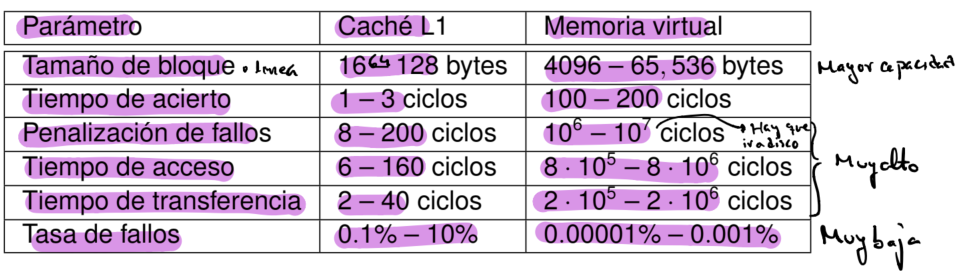
\includegraphics[scale=.4]{Untitled 28.png}}
        \end{figure}
      \end{itemize}
    \end{itemize}

 \section{Políticas de memoria virtual}

  \begin{itemize}
  \item
    Ubicación de página:
  \item
    Correspondencia totalmente asociativa: Las páginas se pueden ubicar
    en cualquier marco de página de memoria principal.

    \begin{itemize}
    
    \item
      Se divide el programa en páginas, y dividimos la memoria principal
      en marco de página.
    \end{itemize}
  \item
    Gestionado por el sistema operativo.

    \begin{itemize}
    
    \item
      Objetivo: Minimizar la tasa de fallos.

      \begin{itemize}
      
      \item
        Penalización muy alta debida a lentitud de discos.
      \item
        En cuanto la penalización por fallo no se puede hacer mucho.
      \end{itemize}
    \end{itemize}
  \item
    Identificación de página:

    \begin{itemize}
    \item
      Se almacena una tabla de páginas por proceso en la memoria
      principal.
    \item
      La tabla tiene la correspondencia entre Identificador de página e
      Identificador de marco de página.

      \begin{figure}[H]
        \ffigbox[\FBwidth]
        {\caption{Identificación de página}}
        {
\includegraphics[scale=.65]{Untitled 29.png}}
      \end{figure}
    \item
      Reducción de tiempo de traducción.
    \end{itemize}
  \item
    TLB -- Translation Lookaside Buffer -- Tabla de Traducción
    Adelantada: Para almacenar más rápido a las traducciones frecuentes y
    no leer memoria.

    \begin{itemize}
    
    \item
      Evita accesos a la tabla de páginas de memoria principal.
    \end{itemize}
  \item
    Remplazo de página:

    \begin{itemize}
    
    \item
      Típicamente LRU -- Menos Reciente Usado.
    \item
      Definida por el Sistema Operativo.
    \item
      Bit de uso: Se activa cuando se accede a la página, y
      periódicamente se pone a 0 el bit de esta manera sabemos lo
      recientemente que se han usado.
    \end{itemize}
  \item
    Estrategia de escritura:

    \begin{itemize}
    
    \item
      Siempre es write-back, escritura retrasada.
    \item
      Hace uso de dirty bit, indicando si se ha modificado una página.
    \item
      El write-through es demasiado lento.
    \item
      El coste de escritura en disco es tremendamente alto.
    \end{itemize}
  \end{itemize}

  \section{Tabla de páginas}

  Las páginas de cada proceso apuntan al marco donde están los datos, en
  virtual parecen ordenados, pero se van asignando según se liberan.

    Proceso de traducción:
    \begin{itemize}

  \item Se tiene una dirección virtual, que contiene: Identificador de
    página virtual y desplazamiento dentro de la página.

    Para páginas de 4 kB necesito 12 bits para el desplazamiento.

    
    
    \item
      Se coge el identificador de página virtual, y se consulta esa
      dirección de la tabla de páginas.
    \item
      La entrada de tabla de páginas contiene: V bit de validez,
      Protección (permisos rwx, \ldots) y dirección de marco de página.
  \item
    Se saca la dirección de marco de página y se junta con el
    desplazamiento de página, de esta manera tenemos la dirección física
    para memoria principal.
    \begin{figure}[H]
      \ffigbox[\FBwidth]
      {\caption{Tabla de páginas}}
      {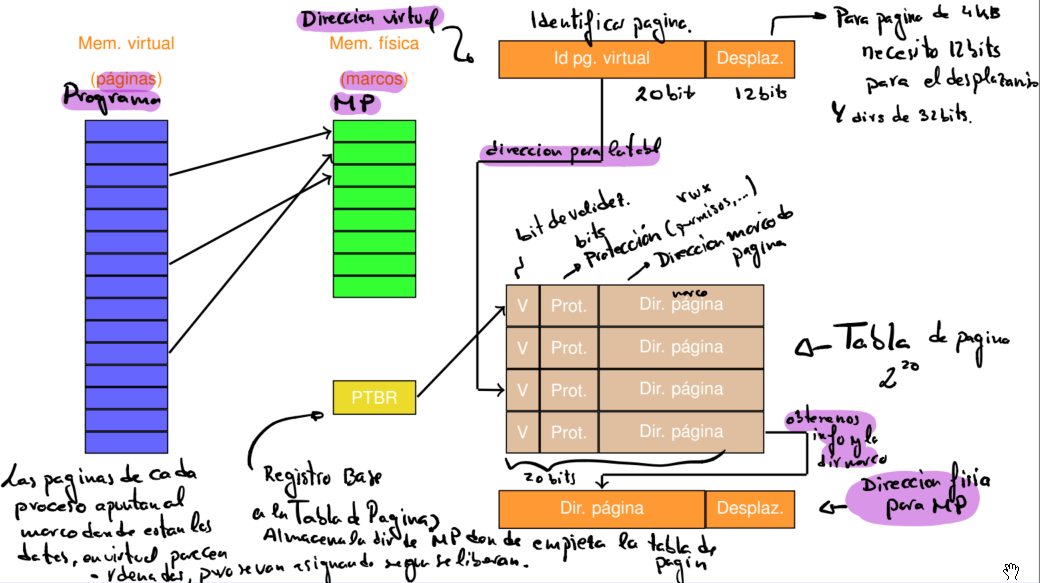
\includegraphics[scale=.35]{Untitled 30.png}}
    \end{figure}
  \end{itemize}
  Se tiene un PTBR -- Registro Base a la Tabla de Página, donde se
  almacena la dirección de memoria principal donde se empieza la tabla
  de página.

  El tamaño de tabla de páginas es, el número de página (número de
  direcciones/tamaño de página) por el tamaño de la entrada.
$$\frac{2^{32}}{2^{12}} \times 2^2 B = 2^22 B = 4 MB$$
  \begin{itemize}
    \item Alternativas:
    \begin{itemize}
      \item Tablas de páginas multinivel: Organización en forma de árbol.
      \item Tablas de páginas invertidas: Va en sentido contrario. Marco —> página.
    \end{itemize}
    
  \end{itemize}

  
    Cada acceso a memoria requiere dos accesos: Acceso a tabla de
    páginas y acceso a memoria.

    TLB -- Translation Lookaside Buffer: Es una caché de traducciones
    frecuentes para evitar accesos a la tabla de páginas.

    \begin{itemize}
    
    \item
      Etiquetas: Porción de dirección virtual.
    \item
      Datos: Número de marco, bits de protección, bit de validez y
      dirty-bit.
    \end{itemize}

    \pagebreak
\section{Máquinas virtuales}

    Desarrollo a finales de los 60, desde entonces se usa en entornos
    mainframe.

    
  Ignoradas en máquinas monousuario hasta finales de los 90.

  
    Se popularizó debido a:
    \vspace{-0.5cm}

    \begin{itemize}
    
    \item
      Importancia del creciente de aislamiento y seguridad en sistemas
      modernos.
    \item
      Fallos en seguridad y fiabilidad en sistemas operativos.
    \item
      Compartición de un computador por varios usuarios.
    \item
      Gran incremento en prestaciones de procesadores.
    \end{itemize}

    Características:
    \vspace{-0.5cm}

    \begin{itemize}
    
    \item
      Ofrecer un entorno idéntico al entorno original para el programa.
    \item
      Los programas corren en el entorno como mucho un poco más lento.
    \item
      Se tiene control completo de los recursos.
    \end{itemize}

    Virtualización: Cualquier método de emulación que ofrece una
    interfaz software estándar con la máquina física.

    Máquinas virtuales de sistema: Ofrecen un entorno completo de
    sistema a nivel de ISA binaria (a nivel de instrucción).

    \begin{itemize}
    
    \item
      Se suele asumir que ISA de MV e ISA de hardware son idénticas.
    \end{itemize}

    Máquina virtual: Ofrece la ilusión de que los usuarios tienen un
    computador completo.
    \vspace{-0.5cm}

    \begin{itemize}
    
    \item
      Un computador ejecuta varias máquinas virtuales, varios sistemas
      operativos y todos compartiendo hardware.
    \item
      Host -- Anfitrión: Plataforma hardware subyacente.
    \item
      Guest -- Invitado: Máquinas virtuales que comparten recursos.
    \end{itemize}

    MMV: Capa de software de sistema.
\vspace{-0.5cm}
    \begin{itemize}
    
    \item
      El monitor se ejecuta sobre la plataforma hardware.
    \item
      Permite la ejecución de varias máquinas virtuales sobre hardware
      único.
    \item
      Capa máquina virtual tiene su propio sistema operativo y
      aplicación.
    \item
      Permite ejecutar aplicaciones sin modificarlas.
    \end{itemize}

\section{MMV -- Monitores de máquinas virtuales o Hipervisor}
\begin{figure}[H]
	\ffigbox[\FBwidth]
	{\caption{MMV}}
	{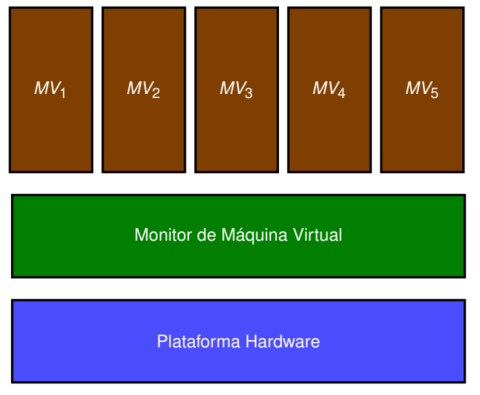
\includegraphics[scale=.6]{Untitled 32.png}}
\end{figure}
  

    Es el software que soporta las máquinas virtuales.

    
  Determina la correspondencia entre recursos virtual y recursos
  físicos.

 
  
    Alternativas en compartición de recursos físicos:

    \begin{itemize}
    
    \item
      Compartición de tiempo. Asignar rodajas de tiempo.
    \item
      Repartir espacio de disco con las máquinas virtuales.
    \item
      Emulado por software.
    \end{itemize}

    Es más pequeño que un sistema operativo tradiciones, ya que no
    necesita todas las funcionalidades.

    Sobrecarga:

    \begin{itemize}
    
    \item
      Depende de la carga de trabajo.
    \item
      Programas ligados a procesadores a nivel de usuario:

      \begin{itemize}
      
      \item
        Ejemplo: SPEC
      \item
        Sobrecarga: 0
      \item
        Raras invocaciones a SO.
      \end{itemize}
    \item
      Programas intensivos en E/S --\textgreater{} intensivos en SO.

      \begin{itemize}
      
      \item
        Muchas llamadas al sistema a instrucciones privilegiadas.
      \item
        Muchas sobrecarga de virtualización.
      \end{itemize}
    \item
      Programas intensivos en E/S y ligados a E/S:

      \begin{itemize}
      
      \item
        Gran parte del tiempo en E/S habría que esperar a estas
        operaciones, y se podrían esconder.
      \item
        Se puede ocultar virtualización.
      \item
        Baja sobrecarga de virtualización.
      \end{itemize}
    \end{itemize}

    Usos:

    \begin{itemize}
    \item
      Aislamiento: Si falla una puede comprometer la otra, para ello los
      aislamos y de esta manera son independientes.
      \begin{figure}[H]
        \ffigbox[\FBwidth]
        {\caption{MMV: Aislamiento}}
        {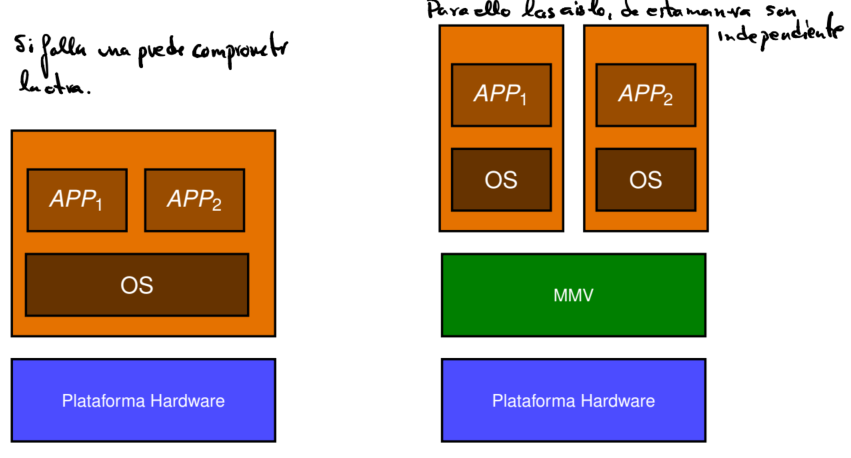
\includegraphics[scale=.3]{Untitled 33.png}}
      \end{figure}
    \item
      Consolidación: Dos máquinas físicas separadas con su propia
      máquina virtual, sistema operativo, apps. Se puede en una misma
      máquina tener ambas máquinas virtuales de esta manera se aprovecha
      más esta máquina.
      \begin{figure}[H]
        \ffigbox[\FBwidth]
        {\caption{MMV: Consolidación}}
        {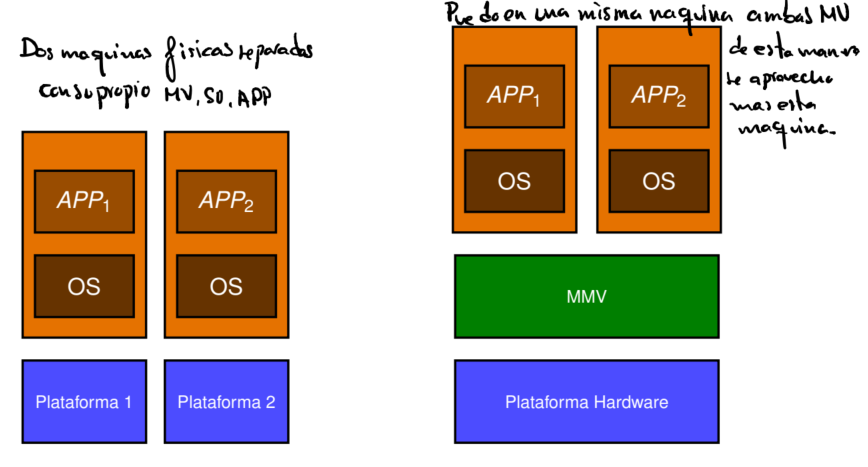
\includegraphics[scale=.3]{Untitled 34.png}}
      \end{figure}
    \item
      Migración: Mover de una máquina a otra.
      \begin{figure}[H]
        \ffigbox[\FBwidth]
        {\caption{MMV: Migración}}
        {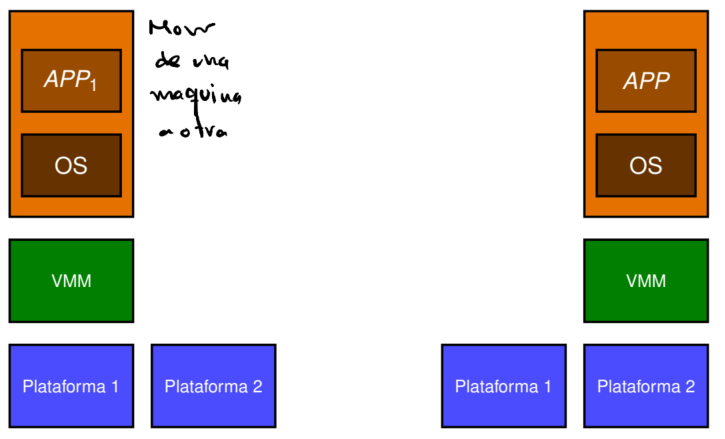
\includegraphics[scale=.3]{Untitled 35.png}}
      \end{figure}
    \end{itemize}

    Otros usos:

    Gestión de software: - MV ofrece una abstracción que permite
    ejecutar pila software completa. - Despliegues combinados SO
    estable, SO heredado y siguiente versión de SO.

    \begin{itemize}
    
    \item
      Gestión de hardware:

      \begin{itemize}
      
      \item
        MV permite ejecutar pilas de software separados, pero sobre un
        mismo hardware.

        \begin{itemize}
        
        \item
          Consolidación de servidores, varios servidores en la misma
          máquina.
        \item
          Independencia a mayor fiabilidad, si falla una puede
          continuar.
        \end{itemize}
      \item
        Migración de MV en ejecución:

        \begin{itemize}
        
        \item
          Equilibrio de carga, se puede mover la carga para reparar o
          traspasar la carga.
        \end{itemize}
      \end{itemize}
    \end{itemize}

    Requisitos de MMV:

    \begin{itemize}
    
    \item
      Una MMV:

      \begin{itemize}
      
      \item
        Presenta una interfaz software a software huésped.
      \item
        Aísla el estado de un huésped del resto.
      \item
        Se protege a sí mismo de los huéspedes.
      \end{itemize}
    \item
      Software huésped se debería comportar como si no hubiese MMV,
      excepto por:

      \begin{itemize}
      
      \item
        Comportamiento dependiente del rendimiento.
      \item
        Limitaciones de recursos fijos compartidos por múltiples MMV.
      \end{itemize}
    \item
      El software huésped no debe poder modificar la asignación de
      recursos reales.
    \item
      MMV debe controlarlo todo:

      \begin{itemize}
      
      \item
        Acceso a estado privilegiado.
      \item
        Traducción de direcciones.
      \item
        E/S.

      \item
        \ldots{}
      \end{itemize}
    \item
      MMV debe ejecutar en un modo más privilegiado que huéspedes.
    \item
      Requisitos de MMV:

      \begin{itemize}
      
      \item
        Como mínimo dos modos de procesador.
      \item
        Subconjunto de instrucciones privilegiadas solo en modo
        privilegiado.
      \end{itemize}
    \end{itemize}

    
\section{Soporte hardware para virtualización}

  \begin{itemize}
  \item
    Soporte de ISA:
  \item
    Si MV se tienen en cuenta en el diseño de ISA, es fácil reducir
    instrucciones que debe ejecutar VMM y cuando tarda la emulación.

    \begin{itemize}
    
    \item
      MMV debe asegurar que huésped solo interacciona con recursos
      virtuales. SO huésped en modo usuario. Los intentos de acceder a
      hardware dan lugar a trap.
    \item
      Si ISA no es consciente de MV, el MMV deben interceptar
      instrucciones problemáticas.
    \end{itemize}
  \item
    Impacto sobre memoria virtual
    \begin{figure}[H]
      \ffigbox[\FBwidth]
      {\caption{Impacto sobre memoria virtual}}
      {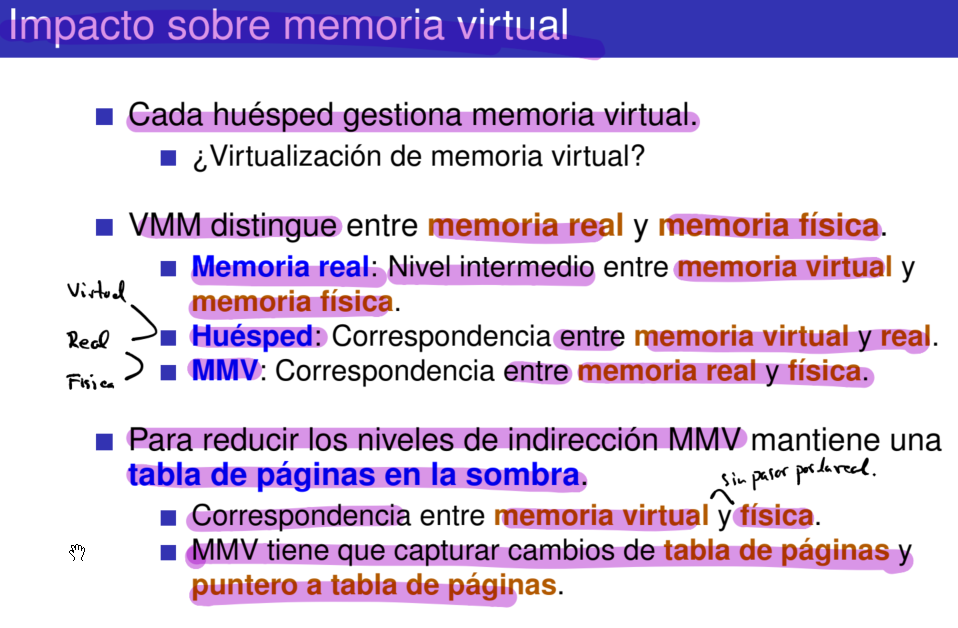
\includegraphics[scale=.3]{Untitled 36.png}}
    \end{figure}
  \item
    Soporte ISA para virtualización de memoria virtual
    \begin{figure}[H]
      \ffigbox[\FBwidth]
      {\caption{Soporte ISA}}
      {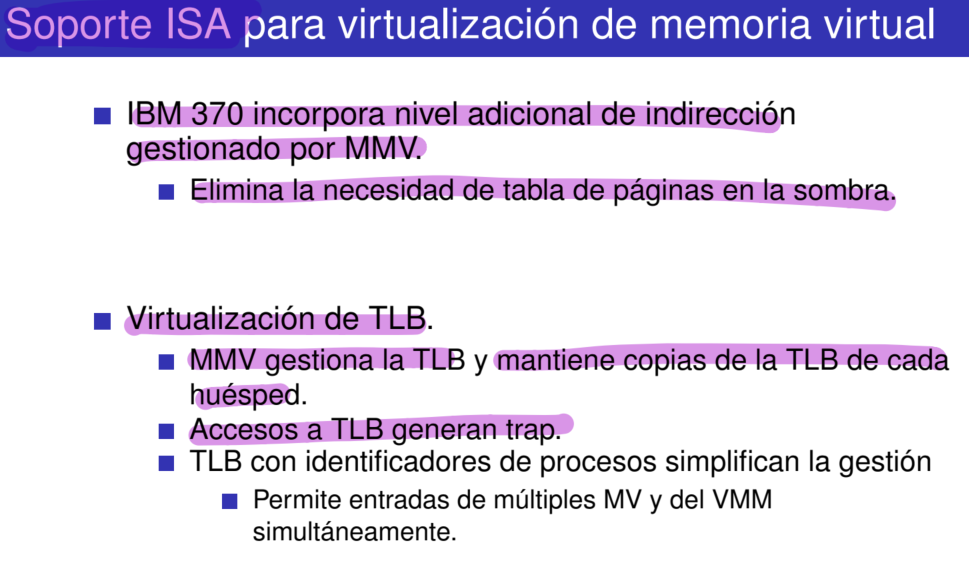
\includegraphics[scale=.4]{Untitled 37.png}}
    \end{figure}
  \item
    Impacto de entrada/salida
    \begin{figure}[H]
      \ffigbox[\FBwidth]
      {\caption{Impacto de entrada/salida}}
      {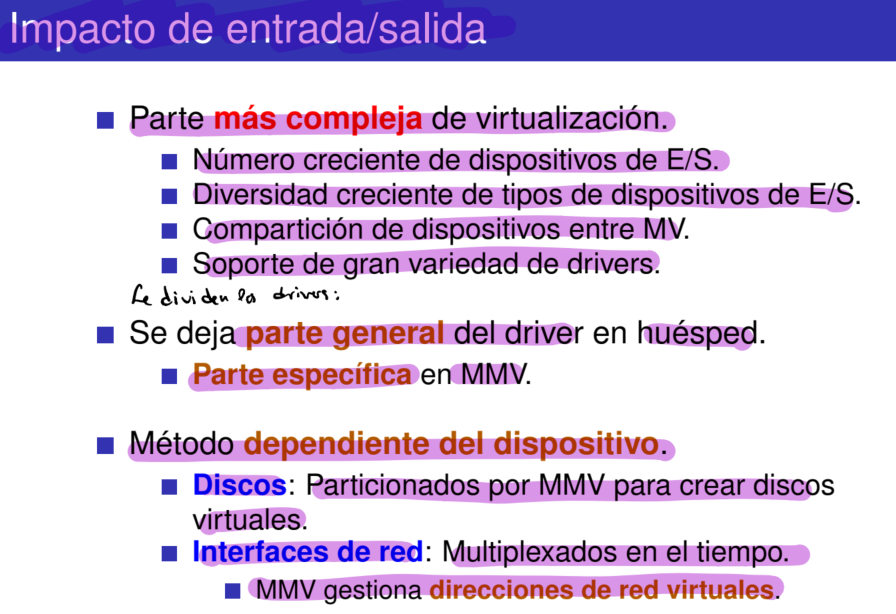
\includegraphics[scale=.4]{Untitled 38.png}}
    \end{figure}
  \end{itemize}
\pagebreak
\section{Tecnologías de virtualización}

  \begin{itemize}
  \item
    Virtualización impura
    \begin{figure}[H]
      \ffigbox[\FBwidth]
      {\caption{Virtualización impura}}
      {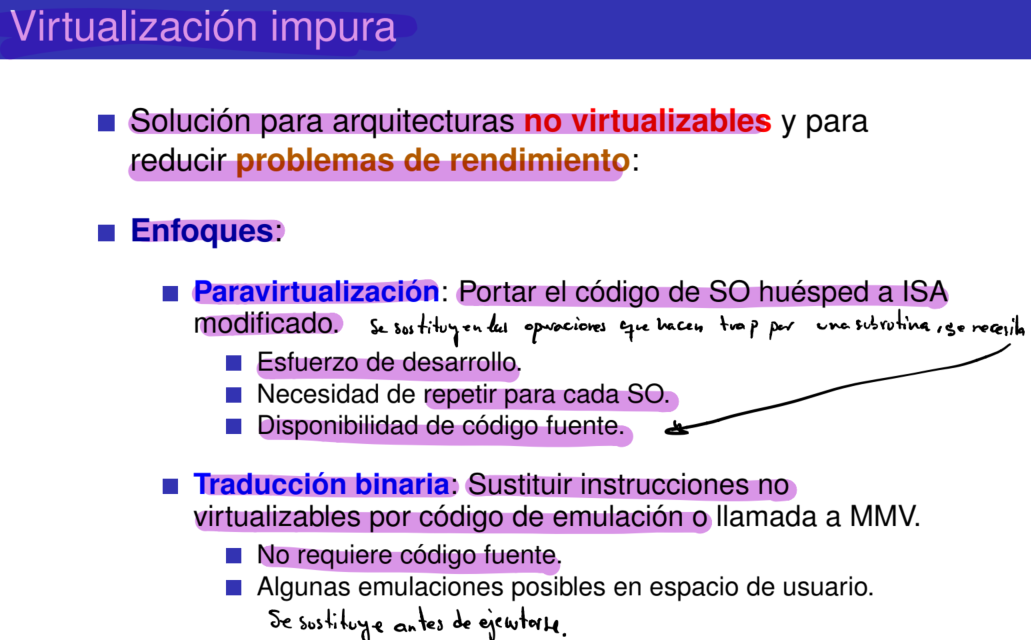
\includegraphics[scale=.4]{Untitled 39.png}}
    \end{figure}
  \item
    Tecnologías ISA
    \begin{figure}[H]
      \ffigbox[\FBwidth]
      {\caption{Tecnologías ISA I}}
      {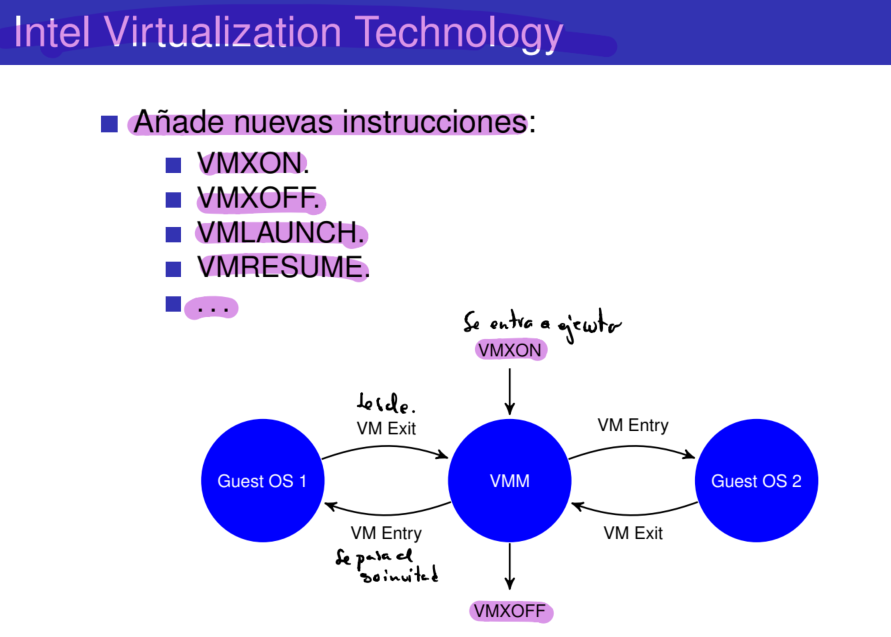
\includegraphics[scale=.4]{Untitled 40.png}}
    \end{figure}
    \begin{figure}[H]
      \ffigbox[\FBwidth]
      {\caption{Tecnologías ISA II}}
      {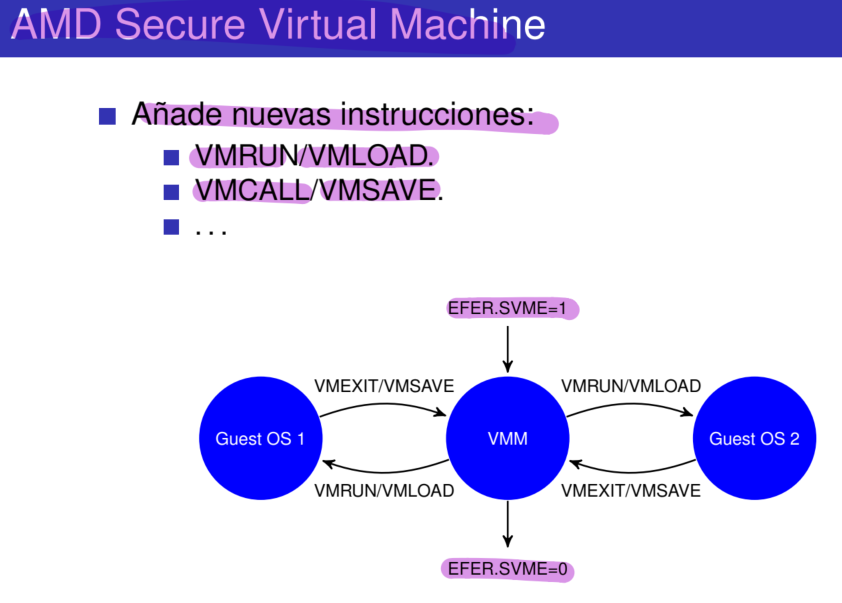
\includegraphics[scale=.4]{Untitled 41.png}}
    \end{figure}
    \begin{figure}[H]
      \ffigbox[\FBwidth]
      {\caption{Tecnologías ISA III}}
      {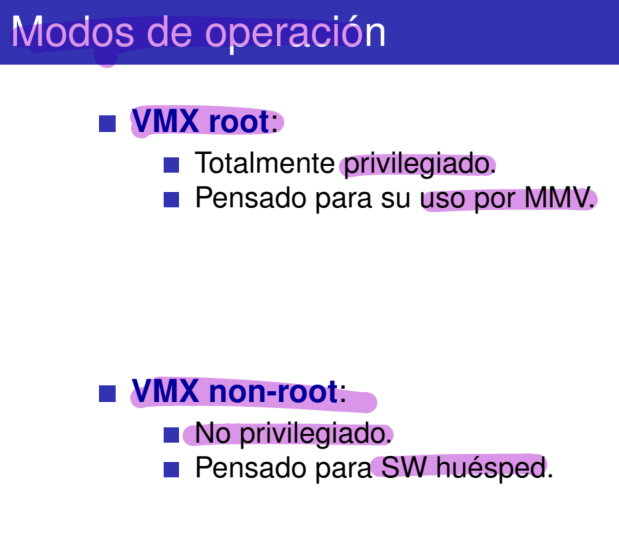
\includegraphics[scale=.4]{Untitled 42.png}}
    \end{figure}
    \begin{figure}[H]
      \ffigbox[\FBwidth]
      {\caption{Tecnologías ISA IV}}
      {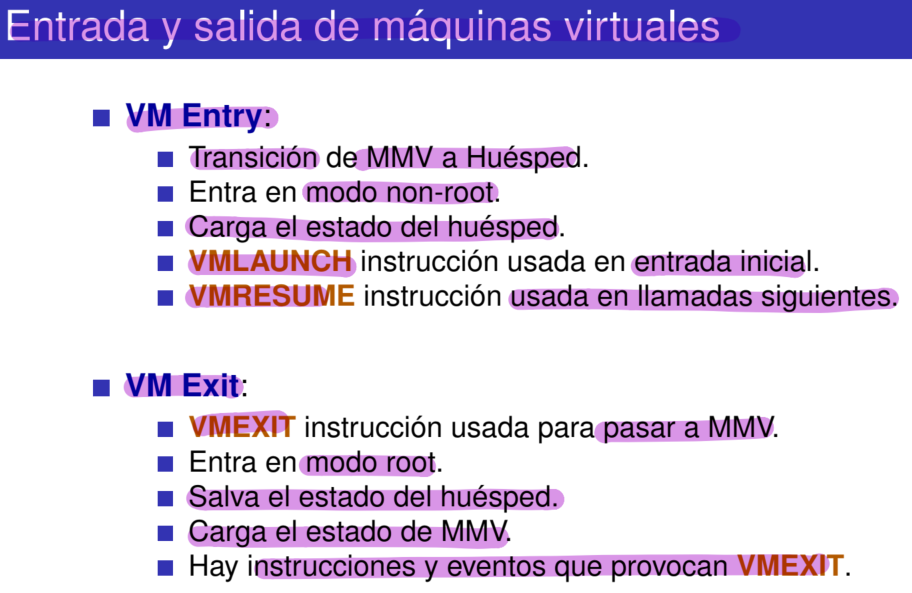
\includegraphics[scale=.4]{Untitled 43.png}}
    \end{figure}
    \begin{figure}[H]
      \ffigbox[\FBwidth]
      {\caption{Tecnologías ISA V}}
      {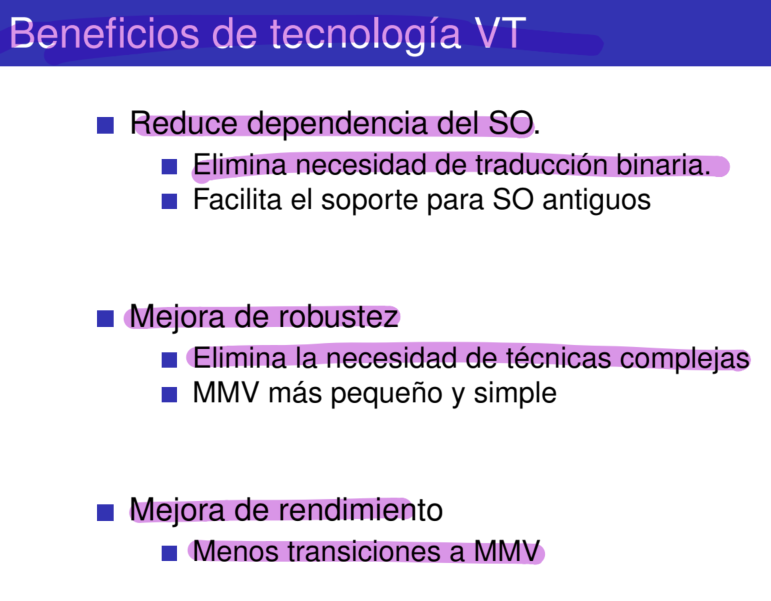
\includegraphics[scale=.4]{Untitled 44.png}}
    \end{figure}
  \end{itemize}

  \chapter{Módulo 5 Introducción a los multiprocesadores}

 \section{Memoria compartida simétrica}


  
\subsection{Introducción a las arquitecturas multiprocesador}


    Creciente importante de multiprocesadores
    \vspace{-0.5cm}

    \begin{itemize}
    
    \item
      Caída de la eficiencia en uso de silicio y energía al explotar
      mayor nivel de ILP.

      \begin{itemize}
      
      \item
        El coste de silicio y energía crece más rápidamente que el
        rendimiento.
      \end{itemize}
    \item
      Interés creciente en servicios de alto rendimiento.

      \begin{itemize}
      
      \item
        Cloud computing, SaaS (Software as a service)
      \end{itemize}
    \item
      Crecimiento de aplicación intensivo en datos.

      \begin{itemize}
      
      \item
        Enormes cantidades de datos en Internet.
      \item
        Big data analytics.
      \end{itemize}
    \end{itemize}

    TLP - Paralelismo a nivel de hilo
    \vspace{-0.5cm}

    \begin{itemize}
    
    \item
      TLP implica la existencia de múltiples contadores de programa.
    \item
      Asume MIMD, múltiples instrucciones sobre múltiples datos.
    \item
      Es reciente que se use TLP fuera de la computación científica.
    \item
      Da lugar a nuevas aplicaciones: Aplicaciones empotradas, Desktop
      y Servidores de alta gama.
    \end{itemize}

    Multiprocesadores
    \vspace{-0.5cm}

    \begin{itemize}
    \item
      Es un computador formado por procesadores altamente acoplados
      con:

      \begin{itemize}
      
      \item
        Coordinación y uso, típicamente controlado por un sistema
        operativo único.
      \item
        Compartición de memoria, tiene un único espacio de direcciones
        compartidas.
      \end{itemize}
    \item
      Modelos de software:

      \begin{itemize}
      
      \item
        Procesamiento paralelo: Hilos acoplados que cooperan. Varios
        hilos haciendo cada uno partes distintas.
      \item
        Procesamiento de peticiones: Ejecución de procesos
        independientes originados por usuarios. Cuando se recibe una
        petición se crea un hilo.
      \item
        Multiprogramación: Ejecución independiente de múltiples
        aplicaciones. Cada hilo ejecuta una aplicación diferente.
      \end{itemize}
      \pagebreak
    \item
      La aproximación más común para alcanzar mejor rendimiento:

      \begin{itemize}
      
      \item
        De 2 a decenas de procesadores.
      \item
        Memoria compartida, no implica una única memoria física.
      \end{itemize}
    \item
      Alternativas:

      \begin{itemize}
      
      \item
        CMP (Chip MultiProcessors) o multi-core: Múltiples chips, que
        pueden ser o no multi-core.
      \item
        Multicomputador o Clúster de computación: Procesadores
        débilmente acoplados que no comparten memoria. Usados en
        computación científica a gran escala.
      \end{itemize}
    \item
      Aprovechamiento de un multiprocesador:

      \begin{itemize}
      
      \item
        Para n procesadores se necesitan n hilos o procesos.
      \end{itemize}
    \item
      Identificación de hilos:

      \begin{itemize}
      
      \item
        Identificados explícitamente por programador.
      \item
        Creados por el sistema operativo.
      \item
        Iteraciones de un bucle generadas por compiladores paralelo.
      \end{itemize}
    \item
      Hilos con un número suficiente de instrucciones a ejecutar. Para
      que merezca la pena arrancar y parar el hilo, tiene que
      compensar.
    \item
      Memoria compartida:

      \begin{itemize}
      
      \item  SMP - Symmetric Multi-Processor:

        \begin{itemize}
          \item Memoria compartida centralizada.

          \item Una memoria centralizada única a la que todos pueden acceder
          por igual.
        
          \item Todos los multi-core son SMP.

          \item UMA - Uniform Memory Access.
          
          Latencia de memoria uniforme.
          \begin{figure}[H]
            \ffigbox[\FBwidth]
            {\caption{Uniform Memory Access}}
            {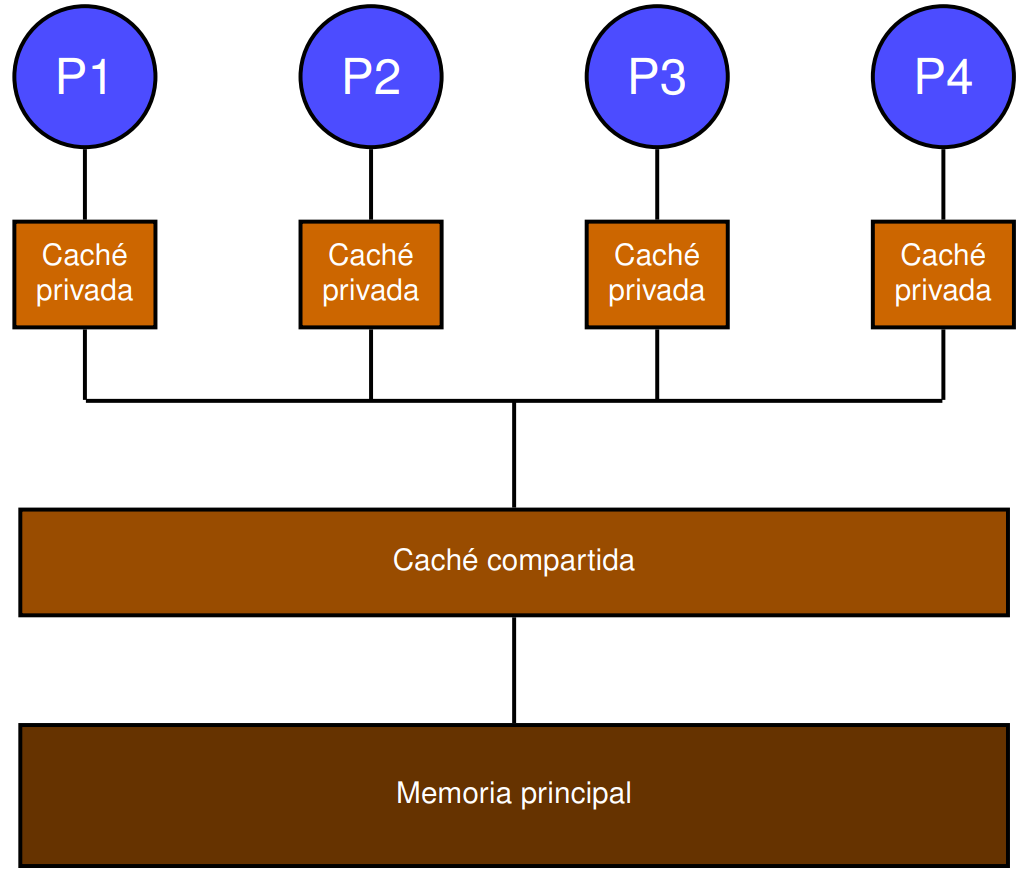
\includegraphics[scale=.15]{Untitled 45.png}}
          \end{figure}
        \end{itemize}
        \pagebreak
      \item DSM - Distributed Shared Memory:
      \begin{itemize}
        \item Memoria compartida distribuida.
        \item La memoria se distribuye entre los procesadores.
        \item Cuando hay muchos procesadores.
        \item NUMA - Non Uniform Memory Access.
            
        Latencia dependiente de la ubicación del dato.
        \begin{figure}[H]
          \ffigbox[\FBwidth]
          {\caption{Non Uniform Memory Access}}
          {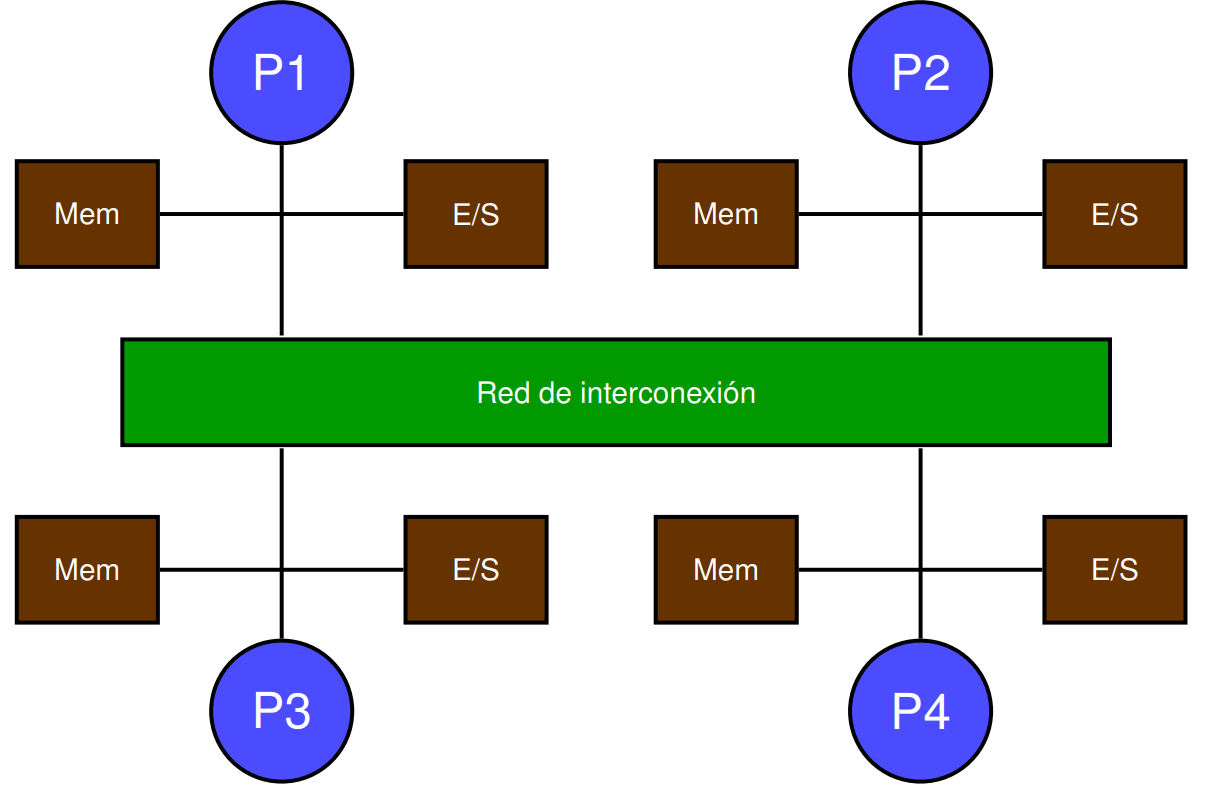
\includegraphics[scale=.15]{Untitled 46.png}}
        \end{figure}
      \end{itemize}
     \end{itemize}

     

\subsection{Arquitecturas de memoria compartida centralizada}

\subsubsection{SMP y jerarquía de memoria}



      Se usa memoria centralizada, porque las caches grandes
      multi-nivel reducen la demanda de ancho de banda sobre memoria
      principal.

      Evolución:

      \begin{enumerate}

        
      \item
        Mono-núcleo con memoria en bus compartido. El bus es
        compartido con periféricos.
      \item
        Conexión de memoria a bus separado solamente para memoria. Uno
        orientado a la memoria y otro a los periféricos lentos.
      \end{enumerate}

      
\subsubsection{Memoria caché}


      
      Tipos de datos en memoria caché:

      \begin{itemize}
      
      \item
        Datos privados: Usados por un único procesador.
      \item
        Datos compartidos: Usados por varios procesadores.
      \end{itemize}

      Problema con datos compartidos:

      \begin{itemize}
      
      \item
        El dato puede replicarse en múltiples caches.
      \item
        Reduce la contención. Cada procesador accede a su copia local.
      \item
        Si dos procesadores modifican sus copias hay que controlar la
        coherencia.

        
          Si modifica su copia local, el otro debe ser consciente del
          mismo.
      \end{itemize}

      Incoherencia de caché

      \begin{itemize}
      
      \item
        Dualidad de estado.

        
          Estado global: Memoria principal.
          Estado local: Cache privada.
      \item
        Un sistema de memoria es coherente si cualquier lectura de una
        posición devuelve el valor más reciente que se haya escrito
        para esa posición.
      \item
        Dos aspectos:
        \begin{itemize}
          \item Coherencia

          \item Consistencia
        \end{itemize}
        

      \end{itemize}

      Condiciones para la coherencia

      \begin{itemize}
      
      \item
        Preservación de orden de programa:

        Una lectura del procesador P sobre la posición X posterior a
          una escritura del procesador P sobre la posición X, sin
          escrituras intermedias de X por otro procesador, siempre
          devuelve el valor escrito por P.

          \item
        Vista coherente de la memoria:


        

        Una lectura de un procesador sobre la posición X posterior a
          una escritura por otro procesador sobre la posición X,
          devuelve el valor escrito si las dos operaciones están
          suficientemente separadas en el tiempo y no hay escrituras
          intermedias sobre X.

          \item
        Serialización de escrituras:


        

        Dos escrituras sobre la misma posición por dos procesadores
          son vistas en el mismo orden por todos los procesadores

        \end{itemize}

        Consistencia de memoria

      \begin{itemize}
      
      \item
        Define en qué momento un proceso que lee verá una escritura.
      \item
        La coherencia y consistencia son complementarias:
        \begin{itemize}
          \item Coherencia: Comportamiento de lecturas y escrituras a una
          única posición de memoria.

          \item Consistencia: Comportamiento de lecturas y escrituras con
          respecto a accesos a otras posiciones de memoria.
        \end{itemize}

        

        
        \end{itemize}
      \end{itemize}

      
\subsection{Alternativas de coherencia de caché}
\subsubsection{Multiprocesadores coherentes:}

 

      Un multiprocesador coherente ofrece:

      \begin{itemize}
      
      \item
        Migración de datos compartidos.

        \begin{itemize}
        
        \item
          Un dato puede moverse a un coche local y usarse de forma
          transparente, que es como si lo hiciera en MP.
        \item
          Reduce latencia de acceso a dato remoto y demanda de ancho
          de banda.
        \end{itemize}
      \item
        Replicación de datos compartidos leídos simultáneamente.

        \begin{itemize}
        
        \item
          Se realiza copia del dato en caché local.
        \item
          Reduce latencia de acceso y contención de las lecturas.
        \end{itemize}
      \end{itemize}

      Propiedades críticas para el rendimiento:

      \begin{itemize}
      
      \item
        La solución debe hacerse mediante hardware, se llaman
        Protocolos de Coherencia de caché.
      \end{itemize}

\subsubsection{Clases de protocolos de coherencia de cache:}

   

      Basado en directorio:

      \begin{itemize}
      
      \item
        En una tabla pública donde se almacena el estado de cada
        bloque de caché de cada procesador.
      \item
        El estado de compartición se mantiene en un directorio.
      \item
        SMP: Directorio centralizado en memoria o en caché de más alto
        nivel compartido.
      \item
        DSM: Para evitar cuello de botella se usa un directorio
        distribuido, cada parte del directorio puede estar en un
        procesador distinto.
      \end{itemize}

      Snooping (espionaje)

      \begin{itemize}
      
      \item
        Cada caché mantiene el estado de compartición de cada bloque
        que tiene.
      \item
        Las caches accesibles mediante medio de multidifusión (bus,
        donde se puede hacer broadcast), los nodos lo estarán
        observando para ver si es válido.
      \item
        Todas las caches monitorizan el medio de multidifusión para
        determinar si tienen una copia del bloque.
      \end{itemize}

      
\subsection{Protocolo basado en directorio}
\begin{figure}[H]
	\ffigbox[\FBwidth]
	{\caption{Protocolo basado en directorio I}}
	{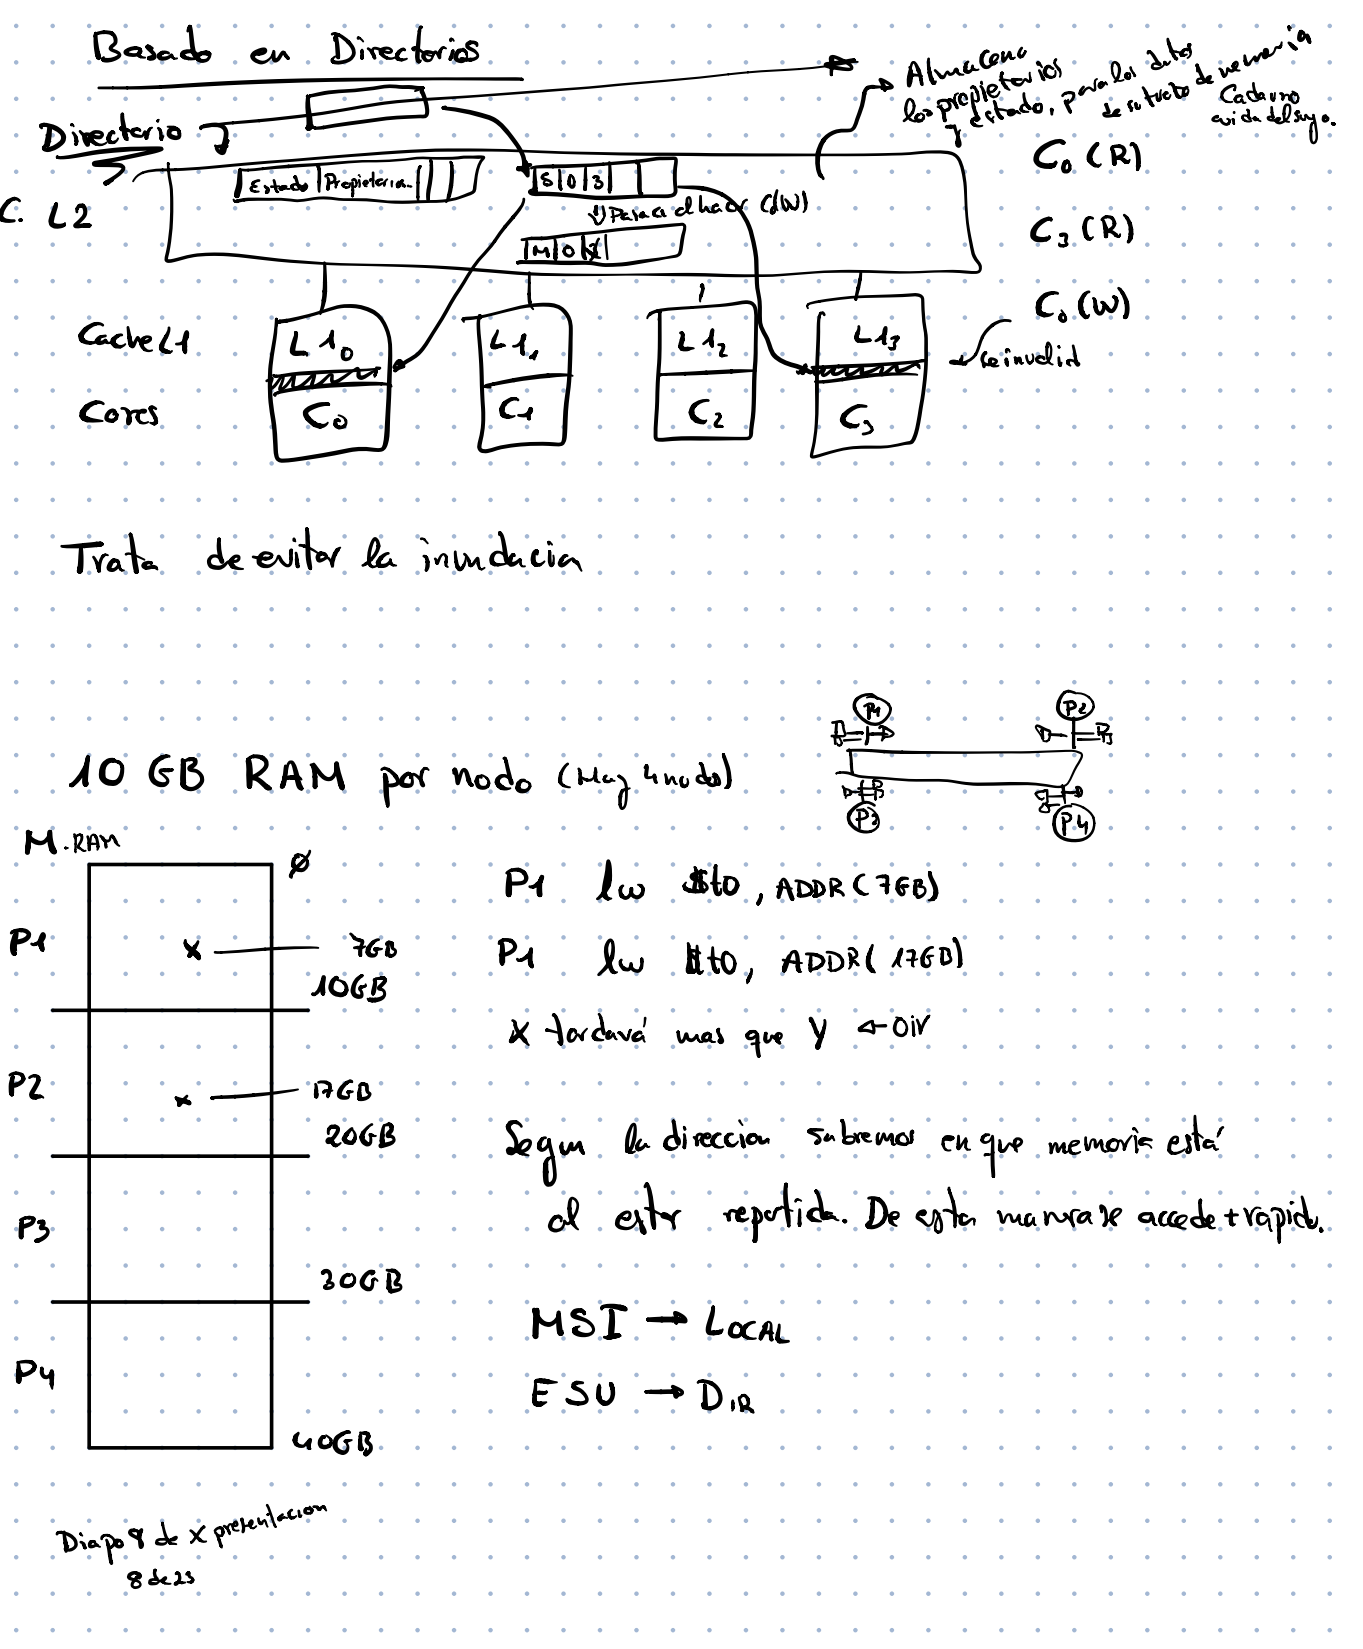
\includegraphics[scale=.3]{Untitled 47.png}}
\end{figure}
\begin{figure}[H]
	\ffigbox[\FBwidth]
	{\caption{Protocolo basado en directorio II}}
	{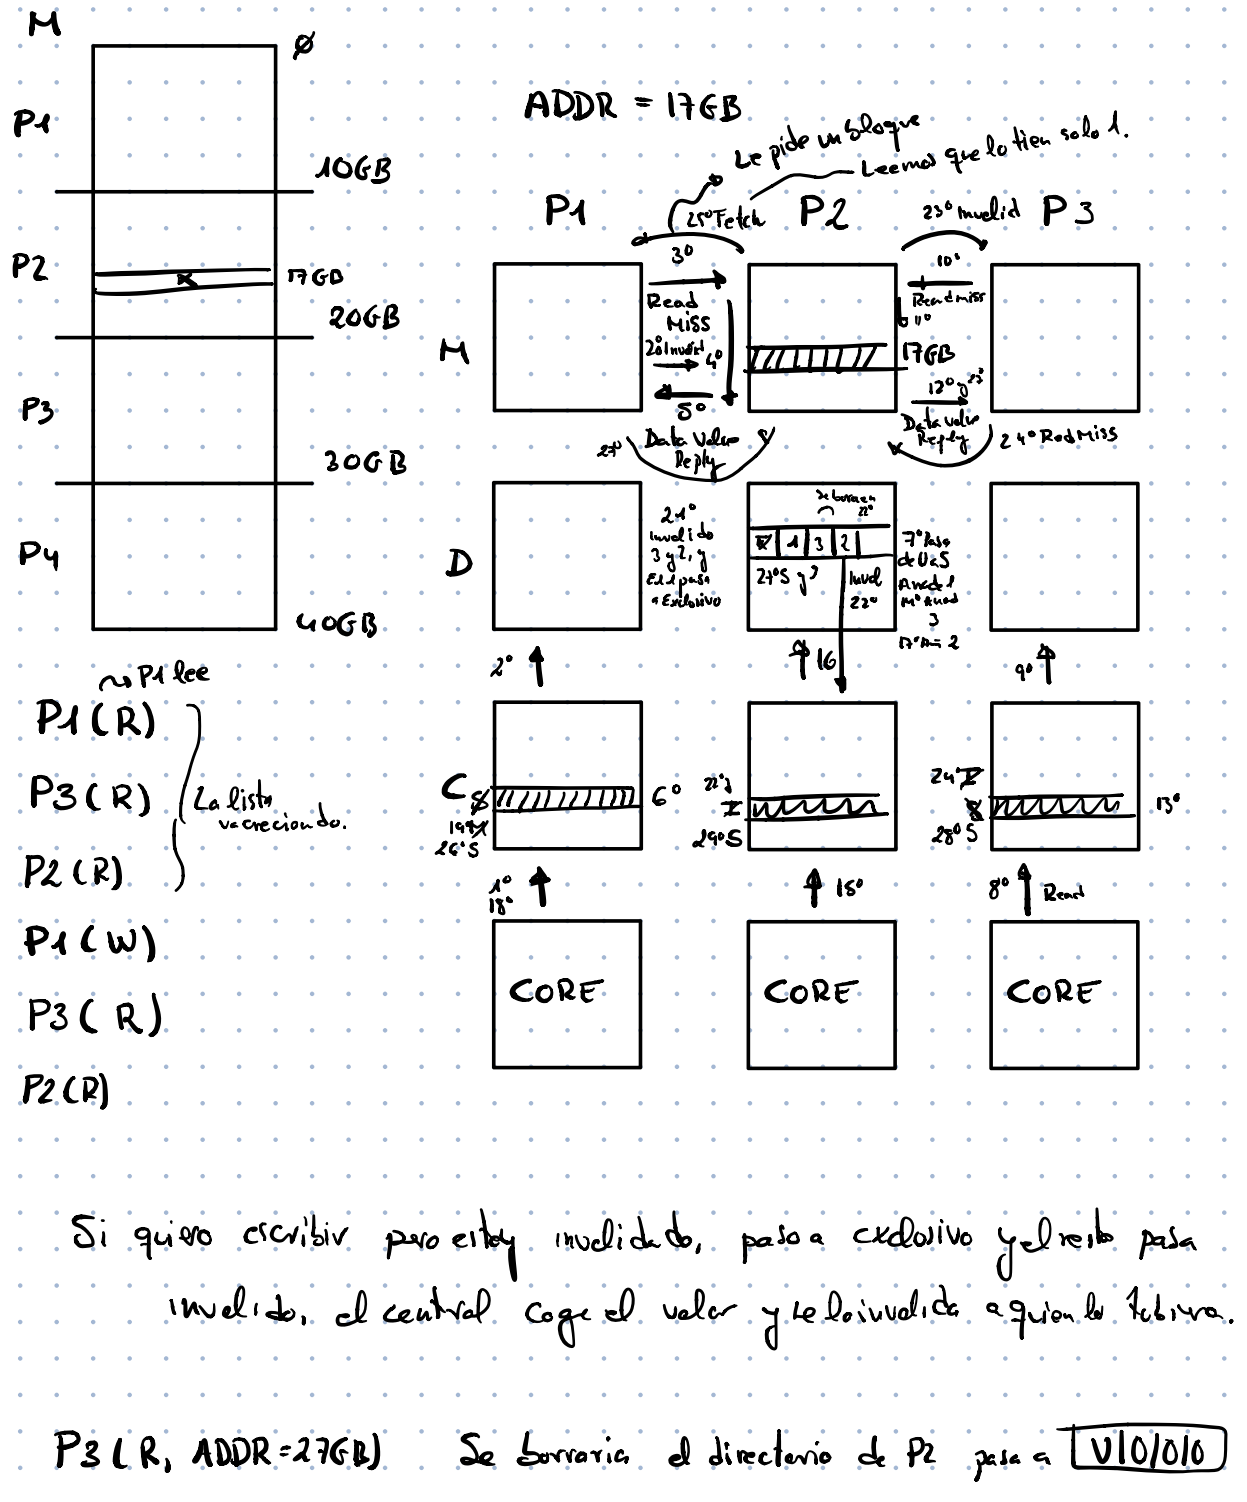
\includegraphics[scale=.3]{Untitled 48.png}}
\end{figure}
\pagebreak
\subsection{Protocolos de espionaje}



    Mantenimiento de la caché: La más común es invalidación.

    \begin{itemize}
    
    \item
      Invalidación de escrituras: Garantiza que un procesador tiene
      acceso exclusivo aun bloque antes de escribir en el, para ello
      se invalida el resto de copias.

      \begin{itemize}
      
      \item
        Cuando se modifica, indican al resto que la suya es inválida y
        si lo necesita la debe volver a pedir.
      \end{itemize}
    \item
      Actualización de escrituras (difusión de escrituras):

      \begin{itemize}
      
      \item
        Difunde todas las escrituras a todas las caches para modificar
        el bloque.
      \item
        Consume más ancho de banda.
      \end{itemize}
    \end{itemize}

    Uso del bus de memoria:

    \begin{itemize}
    
    \item
      Invalidación

      \begin{itemize}
      
      \item
        El procesador adquiere el bus y difunde la dirección a
        invalidar.
      \item
        Todos los procesadores espían el bus.
      \item
        Cada procesador comprueba si tienen en caché la dirección
        difundida y la invalida.
      \end{itemize}
    \item
      No puede haber dos escrituras simultáneamente, el uso exclusivo
      de bus serializa las escrituras.
    \item
      Fallos de caché:

      \begin{itemize}
      
      \item
        Escritura inmediata: La memoria tiene la última escritura
        realizada.
      \item
        Post-escritura: Si un procesador tiene copia modificada,
        contesta al fallo de caché del otro procesador.
      \end{itemize}
    \end{itemize}

    Implementación

    \begin{itemize}
    
    \item
      Invalidación: Se aprovecha del bit de validez (V) asociado a
      cada bloque.
    \item
      Escritura:

      \begin{itemize}
      
      \item
        Necesidad de saber si hay otras copias en caché.

        \begin{itemize}
        
        \item
          Si no hay otras copias no hay que difundir escritura.
        \end{itemize}
      \item
        Cuando hay escritura:

        \begin{itemize}
        
        \item
          Se genera invalidación en bus.
        \item
          Se pasa de estado compartido a estado exclusivo.
        \item
          No hace falta enviar nuevas invalidaciones.
        \end{itemize}
      \item
        Cuando hay fallo de caché en otro procesador:

        \begin{itemize}
        
        \item
          Se pasa de estado exclusivo a estado compartido.
        \end{itemize}
      \end{itemize}
    \end{itemize}

    Protocolo básico: MSI

    \begin{itemize}
    \item
      Basado en una máquina de estados para cada bloque de caché:

      \begin{itemize}
      
      \item
        Cambia de estado por: Peticiones del procesador o Peticiones
        del bus.
      \item
        Acciones: Cambiar de estado o Acciones sobre el bus.
      \end{itemize}
    \item
      Tres estados:

      \begin{itemize}
      
      \item
        M: El bloque ha sido modificado.
      \item
        S: El bloque está compartido.
      \item
        I: El bloque ha sido invalidado.
      \end{itemize}
    \item
      Acciones generadas por el procesador
      \begin{figure}[H]
        \ffigbox[\FBwidth]
        {\caption{Acciones del procesador I}}
        {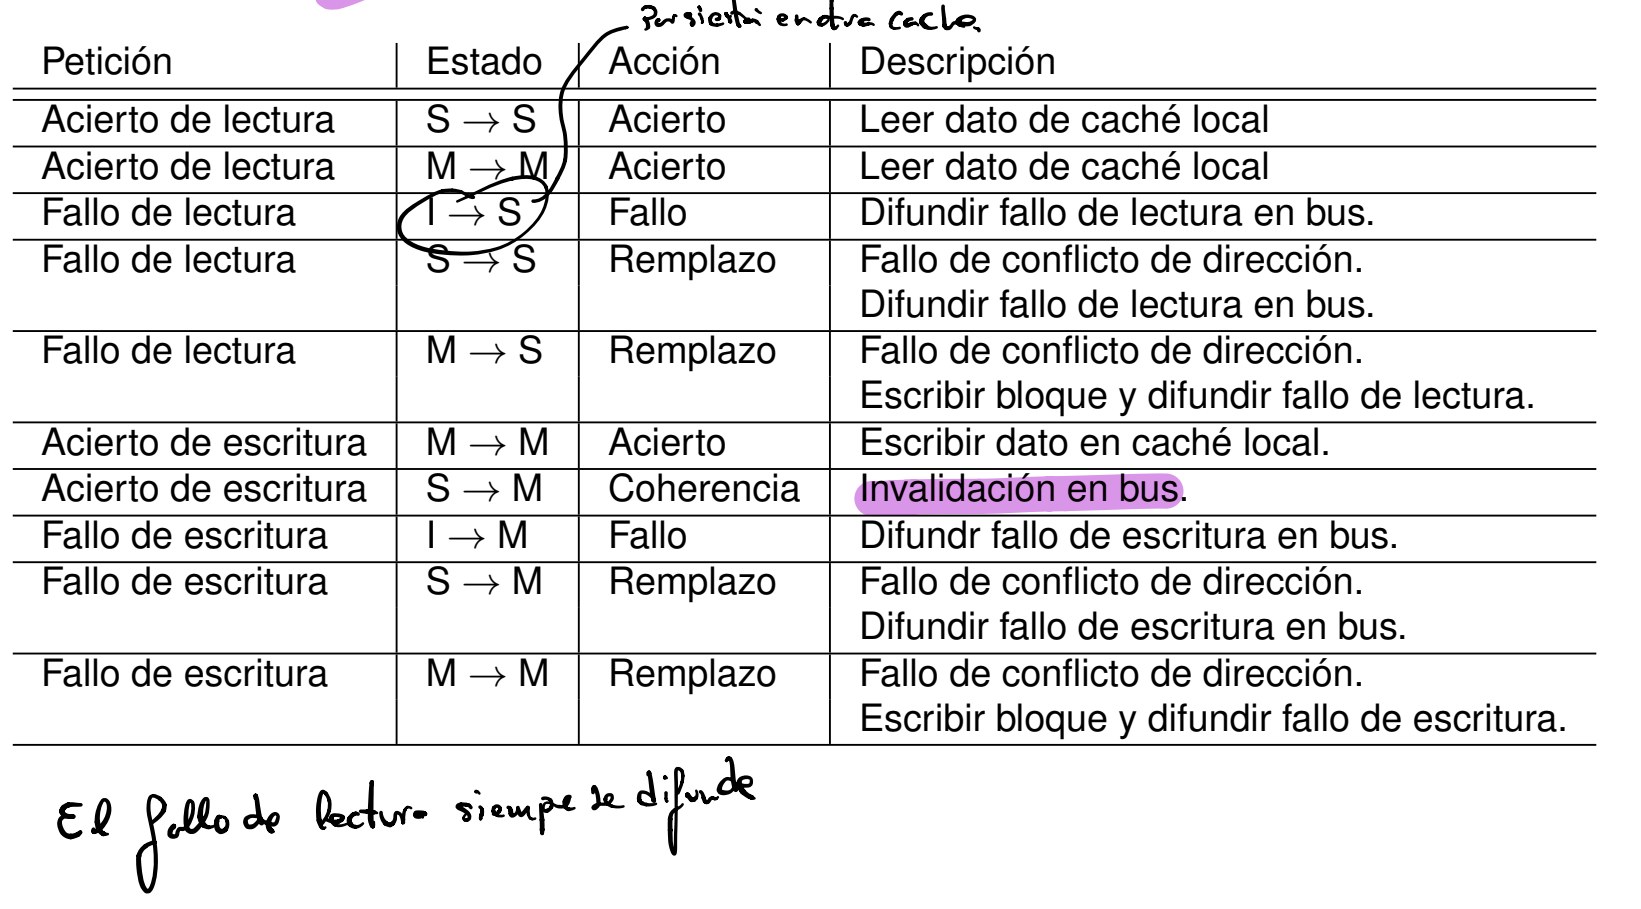
\includegraphics[scale=.2]{Untitled 49.png}}
      \end{figure}
      \begin{figure}[H]
        \ffigbox[\FBwidth]
        {\caption{Acciones del procesador II}}
        {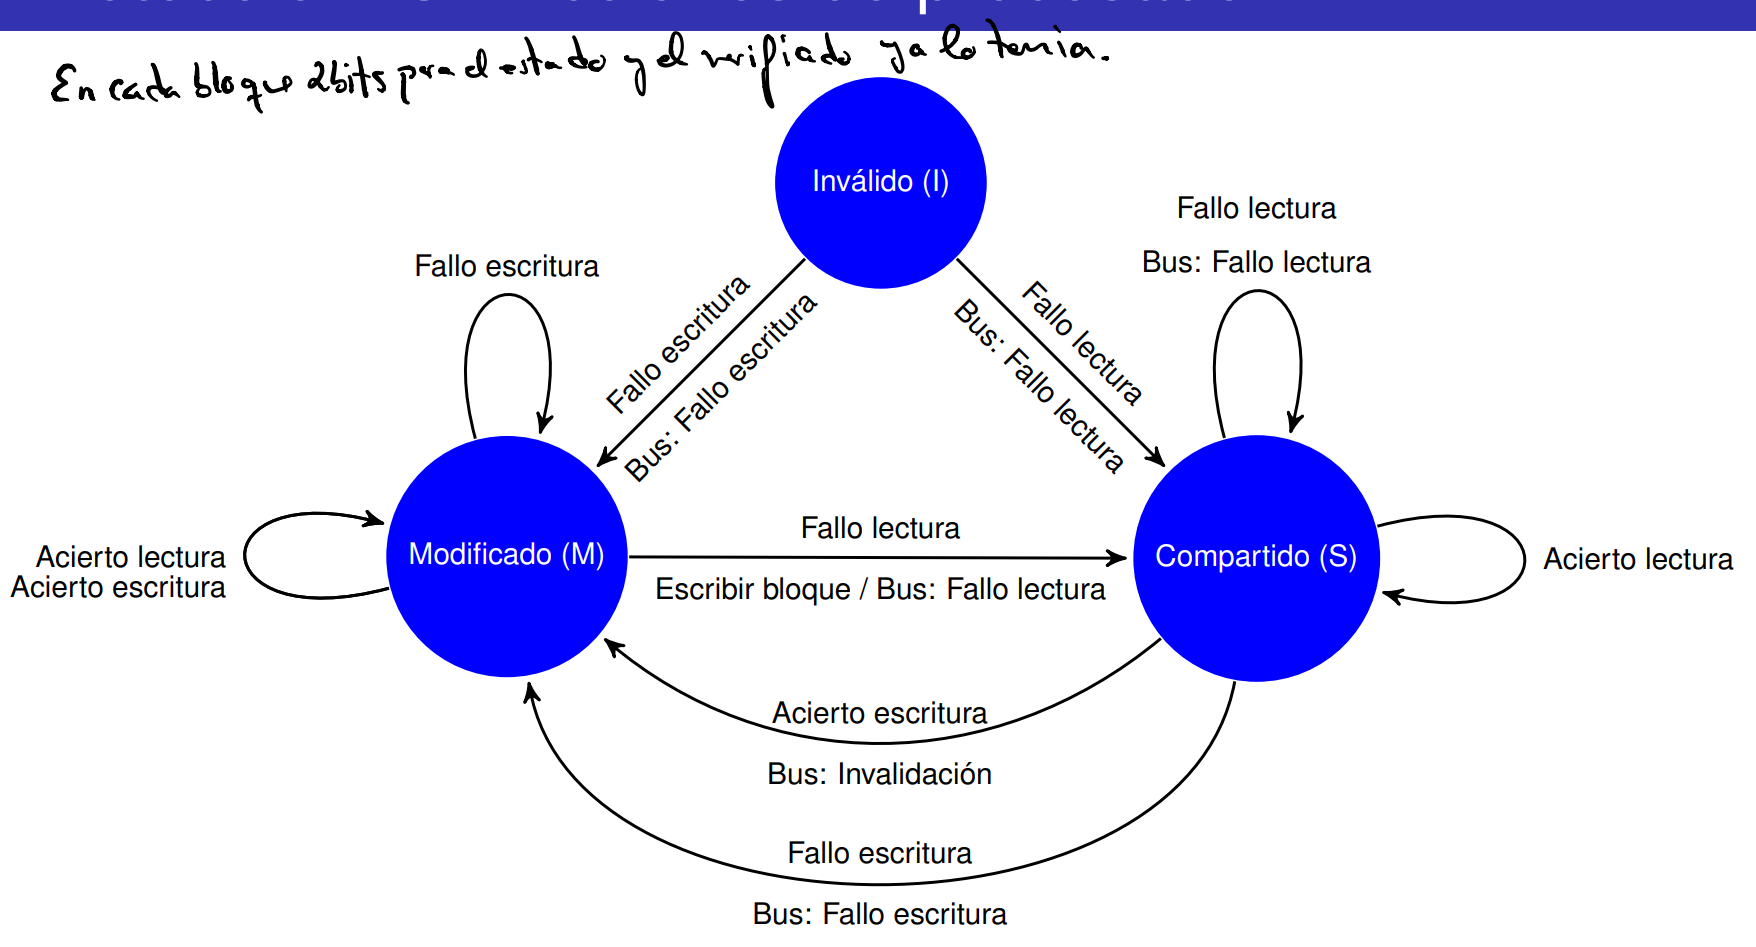
\includegraphics[scale=.2]{Untitled 50.png}}
      \end{figure}
    \item
      Acciones generadas por el bus
      \begin{figure}[H]
        \ffigbox[\FBwidth]
        {\caption{Acciones del bus I}}
        {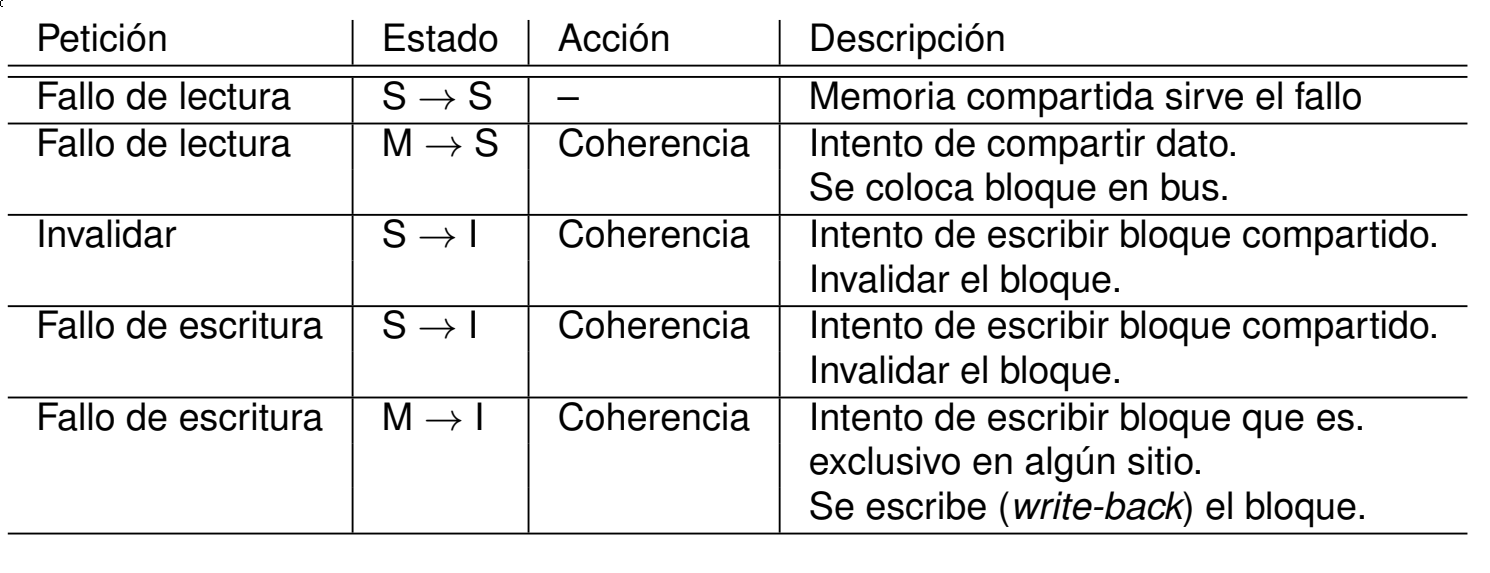
\includegraphics[scale=.2]{Untitled 51.png}}
      \end{figure}
      \begin{figure}[H]
        \ffigbox[\FBwidth]
        {\caption{Acciones del bus II}}
        {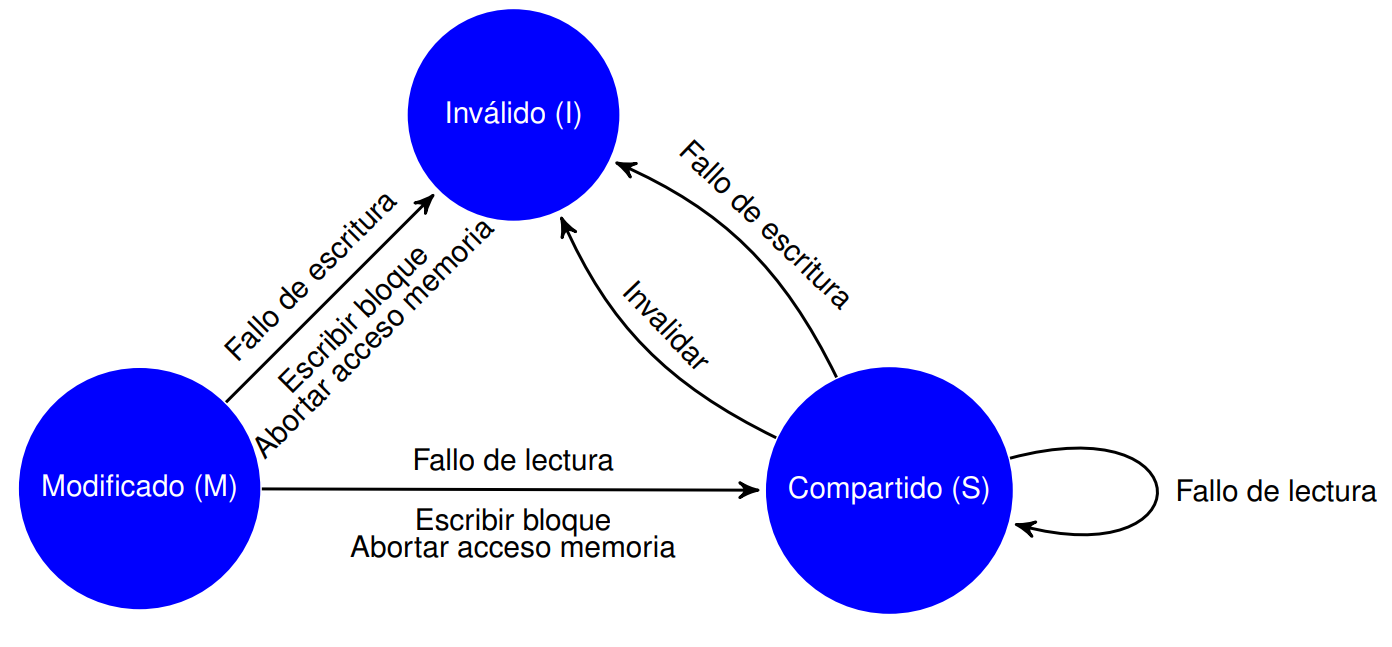
\includegraphics[scale=.2]{Untitled 52.png}}
      \end{figure}
    \item
      Complejidad del protocolo MSI
    \end{itemize}

    Asume que las operaciones son atómicas. - Si las operaciones no
    son atómicas, hay posibilidad de interbloqueo (deadblock) y/o
    carreras.

    La solución el procesador que envía invalidación mantiene
    propiedad del bus hasta que la invalidación llega al resto.

    Extensiones a MSI:

    \begin{itemize}
    
    \item
      MESI: 4 estados.

      \begin{itemize}
      
      \item
        Añade estado exclusivo (E), que indica que reside en una única
        cache pero no está modificado.
      \item
        Escritura de un bloque E no genera invalidaciones.
      \end{itemize}
    \item
      MESIF: 5 estados.

      \begin{itemize}
      
      \item
        Añade además de E, el estado forward (F) que indica que nodo
        debe responder a una petición. Usado en Intel Core i7.
      \end{itemize}
    \item
      MOESI: 5 estados.

      \begin{itemize}
      
      \item
        Añade además de exclusivo, los estados poseídos (O) que indica
        que el bloque está desactualizado. Usado en AMD Opteron.
      \end{itemize}
    \end{itemize}

\subsection{Rendimiento en SMPs}


    El uso de políticas de coherencia de caché tiene impacto sobre
    tasa de fallos.

    Aparecen fallos de coherencia:

    \begin{itemize}
    
    \item
      Fallos de compartición verdadera (true sharing):

      \begin{itemize}
      
      \item
        Un procesador escribe en bloque compartido y lo invalida.
      \item
        Otro procesador lee de bloque compartido y se lo trae.
      \item
        Si el segundo lo modifica invalida al primero, lo que produce
        un ``ping-pong'', se modifican e inválida.
      \end{itemize}
    \item
      Fallos de compartición falsa (false sharing): Es difícil de ver.

      \begin{itemize}
      
      \item
        Un procesador escribe en bloque compartido e inválida.
      \item
        Otro procesador lee una palabra distinta del mismo bloque.
      \item
        Uno lo ha modificado y otro tiene una copia local, ambos del
        mismo bloque.
      \end{itemize}
    \end{itemize}
\pagebreak
    Gráficas:
    \begin{figure}[H]
      \ffigbox[\FBwidth]
      {\caption{Rendimiento en SMPs I}}
      {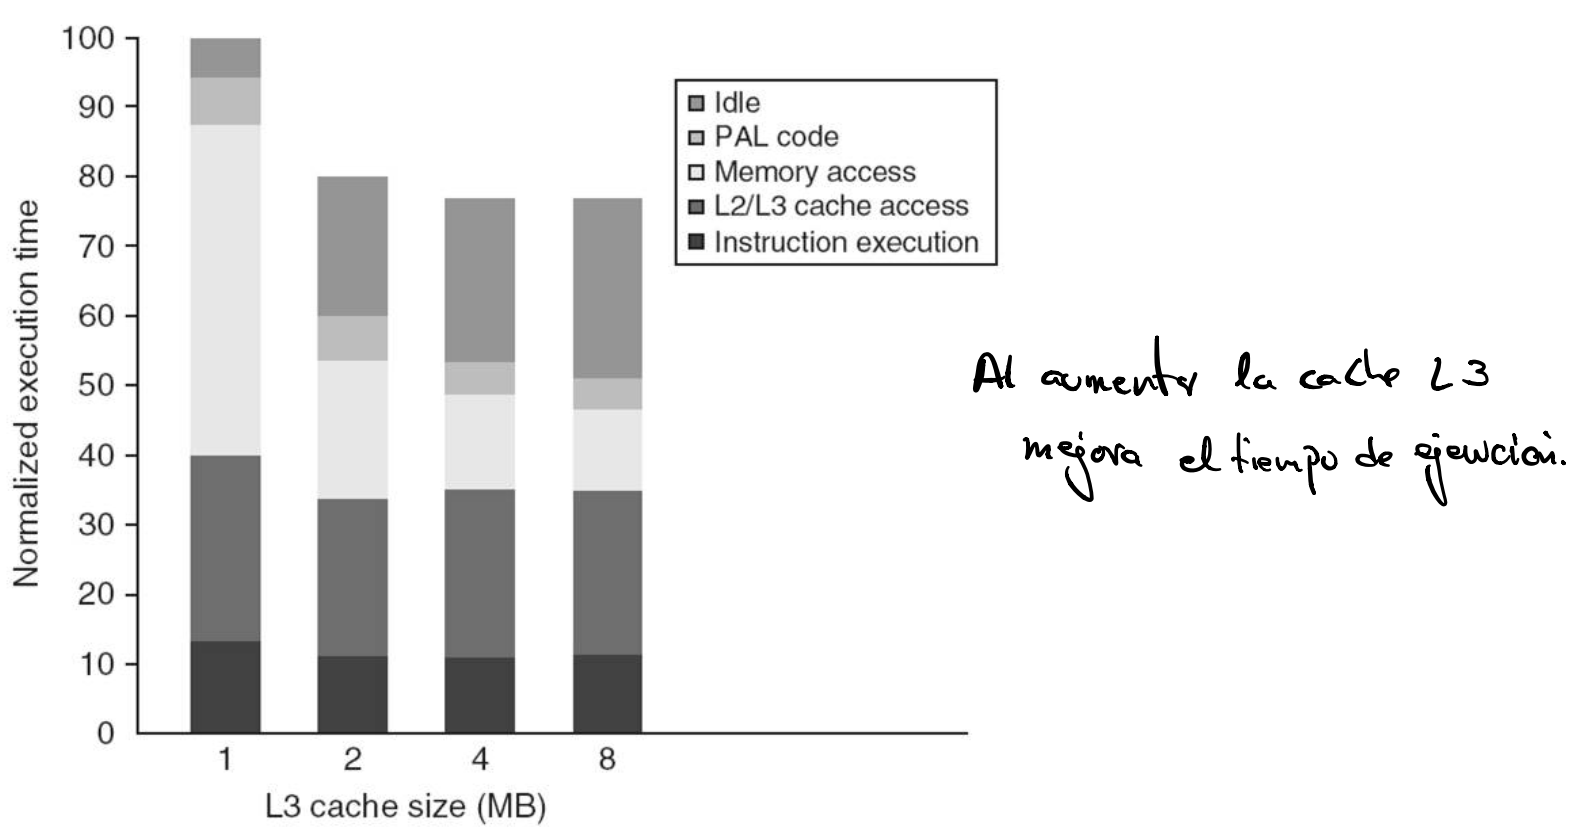
\includegraphics[scale=.15]{Untitled 53.png}\includegraphics[scale=.13]{Untitled 54.png}}
    \end{figure}
    \begin{figure}[H]
      \ffigbox[\FBwidth]
      {\caption{Rendimiento en SMPs II}}
      {\includegraphics[scale=.13]{Untitled 55.png}\includegraphics[scale=.13]{Untitled 56.png}}
    \end{figure}

    
\section{Modelos de consistencia de memoria}


  
\subsection{Modelo de memoria}


    Modelo de consistencia de memoria

    \begin{itemize}
    
    \item
      Conjunto de reglas que define como procesa el sistema de memoria
      las distintas operaciones de memoria de múltiples procesadores.
    \item
      Contrato entre el programador y el sistema, conjunto de reglas y
      condiciones.
    \item
      Determina que optimizaciones son válidas sobre programas
      correctos.
    \end{itemize}

    Modelo de memoria

    \begin{itemize}
    
    \item
      Interfaz entre el programa y sus transformadores.
    \item
      El modelo de memoria del lenguaje tiene implicaciones para el
      hardware.

      \begin{figure}[H]
        \ffigbox[\FBwidth]
        {\caption{Modelo de memoria}}
        {\includegraphics[scale=.5]{Untitled 57.png}}
      \end{figure}
    \end{itemize}

    Modelo de memoria monoprocesadores

    \begin{itemize}
    
    \item
      Las operaciones que nos importan son lecturas y escrituras.
    \item
      Modelo de comportamiento de memoria

      \begin{itemize}
      
      \item
        Las operaciones de memoria ocurren en orden de programa.

        \begin{itemize}
        
        \item
          Lectura devuelve el valor de la última escritura.
        \end{itemize}
      \item
        Semántica definida por orden de programa secuencial:

        \begin{itemize}
        
        \item
          Razonamiento simple pero restringido.

            Resolver dependencias de datos y control.

            \item
          Las operaciones independientes pueden ejecutarse en
          paralelo.
        \item
          Las optimizaciones preservan la semántica.
        \end{itemize}
      \end{itemize}
    \end{itemize}

\subsection{Consistencia secuencial}
\begin{figure}[H]
  \ffigbox[\FBwidth]
  {\caption{Consistencia secuencial}}
  {\includegraphics[scale=.5]{Untitled 58.png}}
\end{figure}


    Un sistema con varios procesadores es secuencialmente consistente
    si para cada posible ejecución las operaciones de memoria que
    genera son equivalentes a las de un programa secuencial en el que
    ponemos esas operaciones en algún orden.

\pagebreak

    Restricciones de la consistencia secuencial

    \begin{itemize}
    \item
      Orden de programa: Si uno de los hilos hace una operación de
      memoria y luego otra, el resto de hilos las deben ver en ese
      mismo orden.

      \begin{itemize}
      
      \item
        Deben hacerse visibles a todos los procesos en el orden de
        programa.
      \end{itemize}
    \item
      Atomicidad: El orden total de ejecución entre procesos debe ser
      consistente requiriendo que todas las operaciones sean atómicas.

      Básicamente no podemos hacer visibles valores que hayan tenido
    encuentra escrituras que todavía no son visibles para el resto.

    \begin{figure}[H]
      \ffigbox[\FBwidth]
      {\caption{Atomicidad}}
      {\includegraphics[scale=.38]{Untitled 59.png}}
    \end{figure}
    \end{itemize}

    

  
    La consistencia secuencial restringe todas las
    operaciones/peticiones de memoria:

    \begin{itemize}
    
    \item
      Write→Read.
    \item
      Write→Write.
    \item
      Read→Read, Read→Write.
    \end{itemize}

    Modelo simple para razonar sobre programas paralelos.

    Hace reordenaciones simples para monoprocesador pueden violar el
    modelo de consistencia secuencial:

    \begin{itemize}
    
    \item
      Reordenación de hardware para mejorar rendimiento.
    \item
      Optimizaciones de compilador aplican transformaciones que
      reordenan operaciones.
    \item
      Transformaciones por programadores o herramientas de refactoring
      también modifican la semántica del programa.
    \end{itemize}
    \pagebreak

    Violación de consistencia secuencial

    \begin{itemize}
    
    \item
      La consistencia secuencial garantiza que no puedan acceder
      simultáneamente a la sección crítica.
    \item
      Si hay escritura en búfer puede que la escritura no llegue a
      memoria a tiempo para que el otro vea el cambio
    \item
      Si las caches usan búfer de escritura:

      \begin{itemize}
      
      \item
        Escrituras se retrasan en búfer.
      \item
        Lecturas obtienen el valor antiguo.
      \item
        Se invalida el algoritmo de Dekker, que es la primera solución
        conocida al problema de exclusión mutua.
      \end{itemize}
    \end{itemize}

    Condiciones para la consistencia secuencial:

    \begin{itemize}
    
    \item
      Cada proceso emite las operaciones de memoria en orden de
      programa.
    \item
      Después de la emisión de una escritura, el proceso de emisión
      espera a que se complete la escritura antes de emitir otra
      operación.
    \item
      Después de emitir una lectura, el proceso que la emitió espera a
      que se complete la lectura y a que la escritura del valor que se
      está leyendo se complete.

      \begin{itemize}
      
      \item
        Esperar la propagación de escrituras.
      \end{itemize}
    \item
      Son restricciones muy exigentes, puede haber condiciones
      necesarias menos exigentes.
    \end{itemize}

\subsection{Otros modelos de consistencia}

 
    Optimizaciones: Modelos que relajan el orden de ejecución de
    problemas.

    \begin{itemize}
    
    \item
      W→R. Se llama Arquitectura de orden de almacenamiento total -
      TSO
    \item
      W→W.
    \item
      R→W, W→W.
    \end{itemize}
\pagebreak
    Ejemplo de modelo comercial, con la restricción que relajan.
    \begin{figure}[H]
      \ffigbox[\FBwidth]
      {\caption{Modelos de consistencia}}
      {\includegraphics[scale=.5]{Untitled 60.png}}
    \end{figure}

    Lectura adelantada a escritura (W→R)

    \begin{itemize}
    
    \item
      Una lectura puede ejecutarse antes que una escritura anterior.
    \item
      Cuando se va a hacer una lectura comprueba el búfer de
      escritura, puede estar ahí el dato modificado.
    \end{itemize}

    Otros modelos:

    \begin{itemize}
    
    \item
      R→W, W→R.

      \begin{itemize}
      
      \item
        Permiten que las escrituras puedan llegar a memoria fuera de
        orden de programa.
      \end{itemize}
    \item
      R→W, W→R, R→R, W→W: El más relajado.

      \begin{itemize}
      
      \item
        Solamente se evitan dependencias de datos y control dentro del
        procesador.
      \item
        Alternativas:

        \begin{itemize}
        
        \item
          Consistencia débil.
        \item
          Consistencia de liberación.
        \end{itemize}
      \end{itemize}
    \end{itemize}

    Consistencia débil

    \begin{itemize}
    
    \item
      Divide las operaciones a memoria en operaciones de datos y
      operaciones de sincronización.
    \item
      Las operaciones de sincronización actúan como una barreara.

      \begin{itemize}
      
      \item
        Todas las operaciones de datos previas deben completarse antes
        de la sincronización.
      \item
        Todas las operaciones de datos posteriores deben esperar a que
        se complete la sincronización.
      \item
        Las sincronizaciones se realizan en orden de programa.
      \end{itemize}
    \item
      Implementación hardware de la barrera

      \begin{itemize}
      
      \item
        Procesador mantiene un contador: De operaciones pendientes,
        así controlamos que todas se han completado.

        \begin{itemize}
        
        \item
          Emisión de operaciones de datos, incrementan el contador.
        \item
          Operaciones de datos completados, decrementa el contador.
        \end{itemize}
      \end{itemize}
    \end{itemize}

    Consistencia de liberación.

    \begin{itemize}
    
    \item
      Más relajada que la consistencia débil.
    \item
      Accesos de sincronización divididos en:

      \begin{itemize}
      
      \item
        Acquire: Adquisición.
      \item
        Release: Liberación.
      \end{itemize}
    \item
      Hace como un bloque que se ejecuta después de acquire y después
      de release.
    \item
      Semántica:

      \begin{itemize}
      
      \item
        Acquire: Debe completarse antes que todos los accesos que lo
        siguen.
      \item
        Release: Debe completarse todos los accesos a memoria previos.

        \begin{itemize}
        
        \item
          Accesos a memoria posteriores SI pueden iniciarse.
        \item
          Operaciones que siguen a release y que deben esperar se
          deben proteger con un acquire.
        \end{itemize}
      \end{itemize}
    \end{itemize}
\pagebreak
\subsection{Caso de uso: Intel}


    Modelo de consistencia

    \begin{itemize}
    
    \item
      Consistencia de memoria en Intel: Hasta el año 2005 Intel no
      había clarificado completamente su modelo de consistencia de
      memoria.

      \begin{itemize}
      
      \item
        Complejidad para formalización del modelo.
      \item
        Problemas para implementaciones de lenguajes.
      \item
        Actualmente el modelo está completamente clarificados y es
        público.
      \end{itemize}
    \item
      I486 y Pentium: Pensado para ejecución secuencial.

      \begin{itemize}
      
      \item
        Operaciones en orden de programa.

        \begin{itemize}
        
        \item
          Excepción: fallos de lectura adelantan escrituras en write
          buffer solamente si todas las escrituras son aciertos de
          caché.
        \item
          Es imposible que el fallo de lectura coincida con una
          escritura.
        \end{itemize}
      \end{itemize}
    \item
      Operaciones atómicas:

      \begin{itemize}
      
      \item
        Desde i486:

        \begin{itemize}
        
        \item
          Leer o escribir 1 byte.
        \item
          Leer o escribir una palabra alineada a 16 bits.
        \item
          Leer o escribir una doble palabra alineada a 32 bits.
        \end{itemize}
      \item
        Desde Pentium:

        \begin{itemize}
        
        \item
          Leer o escribir quadword alineado a 64 bits.
        \item
          Acceso a memoria no cacheada que cabe en bus de datos de 32
          bits.
        \end{itemize}
      \item
        Desde P6:

        \begin{itemize}
        
        \item
          Acceso no alineado a datos de 16, 32 o 64 bits que caben en
          una línea de caché.
        \end{itemize}
      \end{itemize}
    \item
      Bloque del bus:

      \begin{itemize}
      
      \item
        Un procesador puede emitir una señal del bloqueo del bus y
        otros elementos no pueden acceder al bus.
      \item
        Bloqueo automático de bus: Instrucciones que lo hacen.

        \begin{itemize}
        
        \item
          Instrucción XCHG.
        \item
          Actualización de descriptores de segmento, directorio de
          páginas y tabla de páginas.
        \item
          Aceptación de interrupciones.
        \end{itemize}
      \item
        Bloqueo software del bus:

        \begin{itemize}
        
        \item
          Uso del prefijo LOCK en:
        \item
          Instrucciones de comprobación y modificación de bit (BTS,
          BTR, BTC).
        \item
          Instrucciones de intercambio (XADD, CMPXCHG, CMPXCHG8B).
        \item
          Instrucciones aritméticas de 1 operando (INC, DEC, NOT,
          NEG).
        \item
          Instrucciones aritmético-lógicas de 2 operandos (ADD, ADC,
          SUB, SBB, AND, OR, XOR).
        \end{itemize}
      \end{itemize}
    \item
      Instrucciones de barrera:

      \begin{itemize}
      
      \item
        LFENCE:

        \begin{itemize}
        
        \item
          Barrera para load.
        \item
          Cada load previo a LFENCE se hace globalmente visible antes
          que cualquier load posterior.
        \end{itemize}
      \item
        SFENCE:

        \begin{itemize}
        
        \item
          Barrera para store.
        \item
          Cada store previo a SFENCE se hace globalmente visible antes
          que cualquier store posterior.
        \end{itemize}
      \item
        MFENCE:

        \begin{itemize}
        
        \item
          Barrera para operaciones de load/store.
        \item
          Todos los load y store previos a MFENCE son globalmente
          visibles antes que cualquier load o store posterior.
        \end{itemize}
      \end{itemize}
    \item
      Modelo de memoria actual dentro del procesador:

      \begin{itemize}
      
      \item
        Lecturas no adelantan lecturas (R→R).
      \item
        Escrituras no adelantan lecturas (R→W).
      \item
        Escrituras no adelantan escrituras (W→W).
      \item
        Hay excepciones para strings y movimientos no temporales.
      \item
        Lecturas si adelantan escrituras anteriores (W a R) a
        direcciones diferentes.
      \item
        Lecturas/escrituras no adelantan a operaciones de (E/S),
        instrucciones con cerrojo o instrucciones de serialización.
      \item
        Lecturas no pueden sobrepasar LFENCE o MFENCE anteriores.
      \item
        Escrituras no pueden sobrepasar LFENCE, SFENCE o MFENCE
        anteriores.
      \item
        LFENCE no puede sobrepasar lectura anterior.
      \item
        SFENCE no puede sobrepasar escritura anterior.
      \item
        MFENCE no puede sobrepasar lectura o escritura anterior.
      \end{itemize}
    \item
      Modelo de memoria multiprocesador:

      \begin{itemize}
      
      \item
        Cada procesador cumple con reglas anteriores individualmente.
      \item
        Las escrituras de un procesador se observan en el mismo orden
        (pero no al mismo tiempo) por todos los demás.
      \item
        Las escrituras de un procesador NO se ordenan con respecto a
        las escrituras de otros procesadores.
      \item
        La ordenación de memoria es transitiva.
      \item
        Dos escrituras son vistas en un orden consistente por
        cualquier procesador distinto de esos dos.
      \item
        Las instrucciones de cerrojo tienen un orden total.
      \end{itemize}
    \end{itemize}

    Ejemplo:
    \begin{figure}[H]
      \ffigbox[\FBwidth]
      {\caption{Ej. modelo de consistencia I}}
      {\includegraphics[scale=.5]{Untitled 61.png}}
    \end{figure}
    \begin{figure}[H]
      \ffigbox[\FBwidth]
      {\caption{Ej. modelo de consistencia II}}
      {\includegraphics[scale=.5]{Untitled 62.png}}
    \end{figure}
    \begin{figure}[H]
      \ffigbox[\FBwidth]
      {\caption{Ej. modelo de consistencia III}}
      {\includegraphics[scale=.5]{Untitled 63.png}}
    \end{figure}
    \begin{figure}[H]
      \ffigbox[\FBwidth]
      {\caption{Ej. modelo de consistencia IV}}
      {\includegraphics[scale=.5]{Untitled 64.png}}
    \end{figure}
    \begin{figure}[H]
      \ffigbox[\FBwidth]
      {\caption{Ej. modelo de consistencia V}}
      {\includegraphics[scale=.5]{Untitled 65.png}}
    \end{figure}
    \begin{figure}[H]
      \ffigbox[\FBwidth]
      {\caption{Ej. modelo de consistencia VI}}
      {\includegraphics[scale=.5]{Untitled 66.png}}
    \end{figure}
    \begin{figure}[H]
      \ffigbox[\FBwidth]
      {\caption{Ej. modelo de consistencia VII}}
      {\includegraphics[scale=.5]{Untitled 67.png}}
    \end{figure}
    \begin{figure}[H]
      \ffigbox[\FBwidth]
      {\caption{Ej. modelo de consistencia VIII}}
      {\includegraphics[scale=.5]{Untitled 68.png}}
    \end{figure}
    \begin{figure}[H]
      \ffigbox[\FBwidth]
      {\caption{Ej. modelo de consistencia IX}}
      {\includegraphics[scale=.5]{Untitled 69.png}}
    \end{figure}
    \begin{figure}[H]
      \ffigbox[\FBwidth]
      {\caption{Ej. modelo de consistencia X}}
      {\includegraphics[scale=.5]{Untitled 70.png}}
    \end{figure}
    \begin{figure}[H]
      \ffigbox[\FBwidth]
      {\caption{Ej. modelo de consistencia XI}}
      {\includegraphics[scale=.45]{Untitled 71.png}}
    \end{figure}
    \pagebreak
    Efectos del modelo
\begin{itemize}
  \item Consistencia secuencial 

  \begin{itemize}
  \item Load: mov reg, {[}mem{]}
  \item
    Store: xchg {[}mem{]}, reg
  \end{itemize}
  \item
    Consistencia relajada
    \begin{itemize}
  \item
    Load: mov reg, {[}mem{]}

    \item
      Store: mov {[}mem{]}, reg

    \end{itemize}

    \item Consistencia de liberación adquisición 

  \begin{itemize}
  \item Load: mov reg, {[}mem{]}
  \item
    Store: mov {[}mem{]}, reg
  \end{itemize}
\end{itemize}
    

    
\section{Sincronización}


  La comunicación ser realiza a través de memoria compartida, para
  ello es necesario sincronizar accesos a variables compartidas.

  \begin{itemize}
  
  \item
    Para evitar condiciones de carrera y por tanto comportamiento no
    definido.
  \end{itemize}

  \subsection{Alternativas}

  
  
    Comunicación 1-1

    \begin{itemize}
    
    \item
      Asegurar que la lectura se produce después de la escritura.
    \item
      En caso de reutilización, asegurar que escritura se haga después
      de lectura anterior.
    \item
      Necesidad de accesos con exclusión mutua.

      \begin{itemize}
      
      \item
        Solamente uno de los procesos accede a una variable a la vez.
      \end{itemize}
    \item
      Sección crítica: Secuencia de instrucciones que acceden a una o
      varias variables con exclusión mutua. Tratamos de protegerla.
    \end{itemize}

    Comunicación colectiva

    \begin{itemize}
    
    \item
      Necesidad de coordinación de múltiples accesos a variables, las
      escrituras se hacen sin interferencias y las lecturas cuando el
      dato está disponible.
    \item
      Deben garantizarse accesos a variable en exclusión mutua.
    \item
      Debe garantizarse que no se lee resultado hasta que todos hasta
      ejecutado su sección crítica.
    \end{itemize}

\subsection{Primitivas hardware}



    Soporte hardware: Necesidad de fijar un orden global de
    operaciones, ya que un modelo de consistencia puede ser
    insuficiente y complejo. Se puede complementar con operaciones
    lectura-modificación-escritura.

    Test and set (test\_and\_set y clear):

    \begin{itemize}
    
    \item
      Secuencia atómica: Ambos pasos se ejecutan sin interrupciones,
      sé lo que hay antes o después no en medio.

      \begin{itemize}
      
      \item
        Lee posición de memoria en registro.
      \item
        Escribe el valor 1 en la posición de memoria.
      \end{itemize}
    \end{itemize}

    Intercambio (swap):

    \begin{itemize}
    
    \item
      Secuencia atómica:

      \begin{itemize}
      
      \item
        Intercambia los contenidos de una posición de memoria y de un
        registro.
      \end{itemize}
    \item
      Lo que conlleva una lectura y escritura de memoria.
    \item
      Más general que test-and-set
    \end{itemize}

    Captación y operación (fetch-and-XXX)

    \begin{itemize}
    
    \item
      Secuencia atómica:

      \begin{itemize}
      
      \item
        Lee posición de memoria en registro, devolviendo el valor.
      \item
        Escribe en la posición de memoria el resultado de aplicar al
        valor original una operación.
      \end{itemize}
    \end{itemize}

    Comparar e intercambiar (compare-and-exchange):

    \begin{itemize}
    
    \item
      Operación sobre dos variables locales (registro a y b) y una
      posición de memoria (variable x).
    \item
      Secuencia atómica:

      \begin{itemize}
      
      \item
        Lee el valor de x.
      \item
        Si x es igual a registro a, entonces, intercambia x y registro
        b.
      \end{itemize}
    \end{itemize}
\pagebreak
    Almacenamiento condicional (LL/SC):

    \begin{itemize}
    
    \item
      LL Load Linked y SC Store Conditional.
    \item
      Funcionamiento:

      \begin{itemize}
      
      \item
        Si el contenido de una variable leída mediante LL se modifica
        antes de un SC el almacenamiento no se lleva a cabo.
      \item
        Si entre LL y SC ocurre cambio de contexto, SC no se lleva a
        cabo.
      \item
        SC devuelve un código de éxito o fracaso.
      \end{itemize}
    \end{itemize}

\subsection{Cerrojos}



    Mecanismo que asegura la exclusión mutua.

    Dos funciones:

    \begin{itemize}
    
    \item
      Lock(k): Adquiere el cerrojo. Solo lo puede adquirir 1 proceso,
      el resto se ponen en espera. Por más que lleguen se ponen en
      espera.
    \item
      Unlock(k): Libera el cerrojo. Permite a u proceso en espera
      adquirir el cerrojo y si no hay nadie en espera lo deja libre y
      quien llegue lo puede bloquear.
    \end{itemize}

    Mecanismo de espera: 2 alternativas.

    \begin{itemize}
    
    \item
      Espera activa: El proceso queda en bucle que constantemente
      consulta valor de variable de control de espera. No libera el
      procesador.

      \begin{itemize}
      
      \item
        Como el Spin-lock, es un cerrojo sin llamadas al sistema.
      \end{itemize}
    \item
      Bloqueo: El proceso queda suspendido y cede el procesador a otro
      proceso. Cuando se hace unlock se libera un proceso bloqueado.

      \begin{itemize}
      
      \item
        La selección de la alternativa depende del coste.
      \end{itemize}
    \end{itemize}

    Componentes: Tres elementos.

    \begin{itemize}
    
    \item
      Método de adquisición: Intentar adquirir el cerrojo.
    \item
      Método de espera: Espera hasta que se pueda adquirir el cerrojo.
    \item
      Método de liberación: Liberar uno o varios procesos en espera.
    \end{itemize}
\pagebreak
    Cerrojos simples:

    \begin{itemize}
    
    \item
      Variable compartida k con dos valores.

      \begin{itemize}
      
      \item
        0 abiertas y 1 cerrado.
      \end{itemize}
    \item
      Lock(n)

      \begin{itemize}
      
      \item
        Si k es 1, se hace espera activa mientras sea 1.
      \item
        Si k es 0, pasa a k=1.
      \item
        No se debe permitir que 2 procesos adquieran cerrojo
        simultáneamente.
      \end{itemize}
    \end{itemize}

    Retardo exponencial: Se utiliza cuando se hacen muchos accesos a
    memoria durante espera activa, por eso se trata de por cada acceso
    a memoria se incrementa el tiempo de espera.

    \begin{itemize}
    
    \item
      Reducir accesos a memoria.
    \item
      Limitar el consumo de energía.
    \item
      Incrementa exponencialmente el tiempo entre invocaciones del
      intento de bloqueo.
    \end{itemize}

    Sincronización y modificación:

    \begin{itemize}
    
    \item
      Se pueden mejorar prestaciones si se usa la misma variable para
      sincronizar y comunicar. Se evita usar variables compartidas
      solamente para sincronizar.
    \end{itemize}

    Cerrojos y orden de llegada:

    \begin{itemize}
    
    \item
      Problema:

      \begin{itemize}
      
      \item
        Implementaciones simples no fijan orden de adquisición de
        cerrojos. Cuando se libera lo adquiere un proceso aleatorio en
        espera, puede darse inanición si no se escoge entre todos al
        más viejo.
      \item
        Se podría dar inanición.
      \end{itemize}
    \item
      Solución:

      \begin{itemize}
      
      \item
        El cerrojo se adquiera por antigüedad en la solicitud.
      \item
        Garantizar orden FIFO.
      \end{itemize}
    \end{itemize}
\pagebreak
    Cerrojos con etiquetas:

    \begin{itemize}
    
    \item
      Dos contadores:

      \begin{itemize}
      
      \item
        Contador de adquisición: Número de procesos que han solicitado
        el cerrojo.
      \item
        Contador de liberación: Número de veces que se ha liberado el
        cerrojo.
      \item
        Si el contado de adquisiciones y liberaciones son iguales esta
        libre.
      \end{itemize}
    \item
      Lock:

      \begin{itemize}
      
      \item
        Etiqueta: Valor de contador de adquisición.
      \item
        Incrementa contador de adquisición.
      \item
        Espera hasta que el contador de liberación coincida con
        etiqueta.
      \end{itemize}
    \item
      Unlock:

      \begin{itemize}
      
      \item
        Incrementa el contador de liberación.
      \end{itemize}
    \end{itemize}

    Cerrojos basados en colas:

    \begin{itemize}
    
    \item
      Una cola con procesos que esperan para entrar en sección
      crítica.
    \item
      Lock:

      \begin{itemize}
      
      \item
        Comprobar si cola está vacía.
      \item
        Sin un proceso se une a la cola hace espera activa en una
        variable.
      \end{itemize}
    \item
      Unlock:

      \begin{itemize}
      
      \item
        Eliminar proceso de cola.
      \item
        Modificar variable de espera de proceso.
      \end{itemize}
    \end{itemize}
\pagebreak
\subsection{Barreras}

Permite sincronizar varios procesos en algún punto.


    Garantiza que ningún proceso supera la barrera hasta que todos han
    llegado.

    Se usan para sincronizar fases de un programa.

    Barreras centralizadas: Contador centralizado asociado a la
    barrera.

    \begin{itemize}
    
    \item
      Cuando el número de procesos que han llegado a la barrera.
    \item
      Cuando se llega a la función se incrementa el contador, y se
      espera a que el contador llegue al número de procesos a
      sincronizar.
    \end{itemize}

    Barrera simple: Problema si se reúse la barrera en un bucle.

    Barrera con inversión de sentido: Esta barrera si permite
    implementarla en un bucle.

    Barreras en árbol: Implementación simple de barrera no es
    escalable.

    \begin{itemize}
    
    \item
      Contención en el acceso a variable compartida.
    \item
      Estructuración de los procesos de llegada y liberación en forma
      de árbol.
    \end{itemize}

    
  
\section{Memoria compartida distribuida}
\includepdf[pages=-]{docs/es-m5-04-shdist-hout.pdf}


  \chapter{Módulo 6 Modelos de programación paralela y concurrente}

\section{Introducción a C++}

  \includepdf[pages=-]{docs/es-m6-00-Introduction_to_C_-_Computer_Architecture.pdf}

\section{Programación concurrente en C++11}

  \includepdf[pages=-]{docs/es-m6-01-openmp-hout.pdf}

\section{Programación paralela con OpenMP}

  \includepdf[pages=-]{docs/es-m6-02-cppconc-ocw.pdf}

\section{Consistencia de memoria en C++}

  \includepdf[pages=-]{docs/es-m6-03-atomics-hout.pdf}


\part{Práctica}

\chapter{Laboratorio 1}

\includepdf[pages=-]{docs/es-m3-lab-2020.pdf}

  \chapter{Laboratorio 2}


  \includepdf[pages=-]{docs/es-m4-lab-2020.pdf}

  \includepdf[pages=-]{docs/Memoria_Lab2.pdf}
  \chapter{Laboratorio 3}


  \includepdf[pages=-]{docs/es-m5-lab-atomics-2020.pdf}

  \includepdf[pages=-]{docs/Memoria_Lab3.pdf}
  \chapter{POpenMP}
  

  \includepdf[pages=-]{docs/MemoriaOpenMP.pdf}{MemoriaOpenMP.pdf}

  \includepdf[pages=-]{docs/es-m6-lab-omp-img-2020.pdf}

\end{document}